
% WARNING!  Do not type any of the following 10 characters except as directed:
%                &   $   #   %   _   {   }   ^   ~   \   
%
%%
%%  default option for pdfx.sty  if not specified on the command-line.
%\providecommand{\pdfxopt}{a-1b}
%% 
%%  Use  {filecontents}  for the  .xmpdata file before input encoding is specified.
%%
%%%%%%%%%%%%%%%%%%%%%%%%%%%%%%%%%%%%%%%%%%%%%%%%%%%
%\begin{filecontents*}{\jobname.xmpdata}
%	% a macro definition, used below
%	\pdfxEnableCommands{% simple macro definitions can be provided everything expands to characters
%	 \def\RossPete{Ross \& Pete}
%	 }
%	\Title{Linear Algebra (\jobname)}%  *not* set by LaTeX's  \title
%	\Author{Jason Siefken\sep et al.}% *not* set by LaTeX's \author
%	\Subject{Linear Algebra textbook/workbook}
%	\Keywords{linear algebra\sep vectors\sep mathematics\sep textbook} 
%	\Org{University of Toronto}
%	\CreatorTool{LaTeX + pdfx.sty with options \pdfxopt}
%	\Copyright{Jason Siefken}
%	\WebStatement{https://github.com/siefkenj/IBLLinearAlgebra/}% should be URL to copyright statement on the web
%	\CoverDisplayDate{2019}
%	\CoverDate{2019-08-014}%  must be in format  YYYY-MM-DD  or  YYYY-MM
%	\Doi{0.0.0.0}%
%	%
%	% setting the color profile, these reproduce the defaults; use your own, if required 
%	%
%	% RGB is used with PDF/A (4 parameters):
%	\setRGBcolorprofile{sRGB_IEC61966-2-1_black_scaled.icc}{sRGB_IEC61966-2-1_black_scaled}{sRGB IEC61966 v2.1 with black scaling}{http://www.color.org}
%	%
%	%  For Adobe Color Profiles, set the directory for your system
%	%
%	%  e.g.  on Mac OS X
%	%  What is it under Windows ?
%	%
%	\gdef\ColorProfileDir{/Library/Application Support/Adobe/Color/Profiles/Recommended/}
%	% 
%	%  For available profiles, see file  AdobeColorProfiles.tex
%	%  For PDF/X-4p or PDF/X-5pg   see file  AdobeExternalProfiles.tex  
%	%
%	%  Now you can use the macros defined in those files:
%	 \FOGRAXXXIX 
%	%
%	% or CMYK is used with  PDF/X (4 parameters)
%	% \setCMYKcolorprofile{\ColorProfileDir coated_FOGRA39L_argl.icc}{Coated FOGRA39}{FOGRA39 (ISO Coated v2 300\%\space (ECI))}{http://www.color.org}
%\end{filecontents*}

\documentclass{problemset}


% pdfx will set color profile etc. information appropriately, so the pdf renders
% consistently across devices. But, it doesn't work with the xelatex-based tectonics
%\usepackage{ifxetex}
	\usepackage[utf8]{inputenc}
%\ifxetex
%\else
%	\usepackage[a-3u]{pdfx}
%	\hypersetup{hidelinks=true, linkcolor = {0 0 1} }
%\fi

%%%
% import all needed packages and macros
%%%
\usepackage[yyyymmdd]{datetime}
%%
%% All packages and macros needed for the problemsets
%%

\usepackage{amsmath}

\usepackage{lipsum}
%\usepackage{showframe}
%\usepackage{layout}


\usepackage[charter,cal=cmcal]{mathdesign} %different font
%\usepackage{avant}

\usepackage{microtype}
\usepackage{mathtools}
\usepackage{etoolbox}
%\usepackage{amsfonts}
%\usepackage{amssymb}
\usepackage{graphicx}
\usepackage[inline]{enumitem}
\usepackage{xparse}
\usepackage{ifthen}
\usepackage{graphicx}
\usepackage{caption}
\usepackage{subcaption}
\usepackage{color}
\usepackage{tikz}
	\usetikzlibrary{fit}
	\usetikzlibrary{fadings}
	\usetikzlibrary{calc}
	\tikzset{>=latex}
	\usetikzlibrary{cd}
	\usetikzlibrary{spy}
\usepackage{fancyhdr}
\usepackage{calc}
\usepackage{wrapfig}
\usepackage{marginnote}
\usepackage{mparhack}
\usepackage{marginfix}


\usepackage{qrcode}

%\usepackage[
%  linktocpage=false,      % no page numbers are clickable
%  colorlinks=false,       % no color
%  breaklinks=true,        % break URLs
%  bookmarks,              % creates bookmarks in pdf
%  hyperfootnotes=true,    % clickable footnotes
%  pdfborder={0 0 0},      % for removing borders around links
%  bookmarksnumbered=true, % If Acrobat bookmarks are requested, include section numbers.
%  bookmarksopen=false,    % If Acrobat bookmarks are requested, show them with all the subtrees expanded.
%  %hidelinks=true,
%  %linkcolor=blue,
%  %citecolor=blue,
%  %urlcolor=blue,
%  pdfpagemode={UseOutlines}, % show pdf bookmarks (indices) on startup; does not function all the time
%  pdftitle={...}, % title
%  pdfauthor={...}, % author
%  pdfkeywords={...}, % subject of the document
%  pdfsubject={...}, % list of keywords
%  pdfmenubar=true,        % make PDF viewer’s menu bar visible
%  pdfpagelabels,
%]{hyperref}
%\usepackage[hidelinks,]{hyperref}
\usepackage{fnpct} % fancy footnote spacing
\usepackage{bm}
\usepackage{systeme}
\usepackage{datatool}% http://ctan.org/pkg/datatool for sorted lists
\usepackage{xspace}



\usepackage{pgfplots}
\pgfplotsset{compat=newest}
	\usepgfplotslibrary{fillbetween}
%%%
% Useful Linear Algebra macros
%%%
\newcommand{\declarecommand}[1]{\providecommand{#1}{}\renewcommand{#1}}
\declarecommand{\R}{\mathbb{R}}  % we don't care if it's already defined.  We really want *this* command!
\declarecommand{\Z}{\mathbb{Z}}
\declarecommand{\Q}{\mathbb{Q}}
\declarecommand{\N}{\mathbb{N}}
\declarecommand{\C}{\mathbb{C}}
\declarecommand{\d}{\mathrm{d}}
\declarecommand{\dd}{\mathbbm{d}} % exterior derivative
\DeclareMathOperator{\Span}{span}
\DeclareMathOperator{\Img}{img}
\DeclareMathOperator{\Id}{id}
\DeclareMathOperator{\Ident}{\Id}
\DeclareMathOperator{\Vol}{Vol}
\DeclareMathOperator{\VolChange}{Vol\hspace{1.5pt}Change}
\DeclareMathOperator{\Range}{range}
\DeclareMathOperator{\Rref}{rref}
\DeclareMathOperator{\Rank}{rank}
\DeclareMathOperator{\Comp}{\Vcomp}
\DeclareMathOperator{\Vcomp}{v\hspace{1pt}comp}
\DeclareMathOperator{\Null}{null}
\DeclareMathOperator{\Nullity}{nullity}
\DeclareMathOperator{\Char}{char}
\DeclareMathOperator{\Proj}{proj}
\DeclareMathOperator{\Flux}{Flux}
\DeclareMathOperator{\Circ}{Circ}
\DeclareMathOperator{\chr}{char}
\DeclareMathOperator{\Dim}{dim}
\DeclareMathOperator{\Perp}{perp}
\DeclareMathOperator{\Ker}{kernel}
\DeclareMathOperator{\Row}{row}
\DeclareMathOperator{\Col}{col}
\DeclareMathOperator{\Rep}{Rep}
\newcommand{\BasisChange}[2]{[#2\!\leftarrow\!#1]}
\newcommand{\proj}{\Proj}
\newcommand{\rref}{\Rref}
\newcommand{\xhat}{{\vec e_1}}
\newcommand{\yhat}{{\vec e_2}}
\newcommand{\zhat}{{\vec e_3}}
\newcommand{\sbasis}[1]{\vec { e}_{#1}}
\newcommand{\mat}[1]{\begin{bmatrix*}[r]#1\end{bmatrix*}}
\newcommand{\matc}[1]{\begin{bmatrix}#1\end{bmatrix}}
\newcommand{\formarg}[2]{\big(#1;\, #2\big)}
\DeclarePairedDelimiter\abs{\lvert}{\rvert}
\DeclarePairedDelimiter\Abs{\lvert}{\rvert}
\DeclarePairedDelimiter\norm{\lVert}{\rVert}
\newcommand{\Norm}[1]{\norm{#1}}
% just to make sure it exists
\providecommand\given{}
% can be useful to refer to this outside \Set
\newcommand\SetSymbol[1][]{%
	\nonscript\::%
	\allowbreak
	\nonscript\:
	\mathopen{}}
\DeclarePairedDelimiterX\Set[1]\{\}{%
	\renewcommand\given{\SetSymbol[\delimsize]}
	#1
}

\newcommand{\scaledgrid}[1]{%
	\begin{tikzpicture}[scale=#1]
		\draw[thin, white!20!black, dotted] (-4.1,-4.1) grid (4.1,4.1);
		\draw[ <->] (-4.3,0) -- (4.3,0);
		\draw[ <->] (0,-4.3) -- (0,4.3);
	\end{tikzpicture}
}
\newcommand{\scaledshortgrid}[1]{%
	\begin{tikzpicture}[scale=#1]
		\draw[thin, white!20!black, dotted] (-4.1,-2.1) grid (4.1,2.1);
		\draw[ <->] (-4.3,0) -- (4.3,0);
		\draw[ <->] (0,-2.3) -- (0,2.3);
	\end{tikzpicture}
}
\newcommand{\singlegrid}{\scaledgrid{1}}
\newcommand{\doublegrid}{\mbox{\scaledgrid{.9}\scaledgrid{.9}}\par}
\newcommand{\triplegrid}{\mbox{\scaledgrid{.6}\scaledgrid{.6}\scaledgrid{.6}}\par}

% labels for source attributions
\NewDocumentCommand{\beezer}{o}{%
	\IfNoValueTF{#1}{%
		{\color{blue}\sffamily{B}}%
	}{%
		{\color{blue}\sffamily{B}}%  XXX Todo, make this href to the appropriate problem number
	}\xspace%
}
\NewDocumentCommand{\hefferon}{o}{%
	\IfNoValueTF{#1}{%
		{\color{blue}\sffamily{H}}%
	}{%
		{\color{blue}\sffamily{H}}%  XXX Todo, make this href to the appropriate problem number
	}\xspace%
}


% in non-xelatex engines, hyperref is loaded by `pdfx`. If `pdfx` is not loaded, load it here.
%\ifxetex
	\usepackage{hyperref}
%	\hypersetup{hidelinks=true, linkcolor = {0 0 1} }
%\else
%\fi

\usepackage{multido}
	\newcommand{\forLoop}[4][1]{\multido{\i=#2+#1}{#3}{#4}}

\usepackage{tikz}
	\usetikzlibrary{arrows.meta}
	\def\seta{Latex[angle'=45]}%,scale=1.5]}
	\def\setam{Latex[angle'=45,scale=0.75]}
	\def\setaa{Straight Barb[angle'=60,scale=2]}
	\newcommand{\tikzcircle}[2][black,fill=gray]{\tikz[baseline=-0.5ex]\draw[#1,radius=#2] (0,0) circle ;}%

%%%
% Set up the footers to have the correct copyright notices
%%%

\fancypagestyle{siefken}{%
	\fancyhead[LO,RE]{\leftmark}	
	\fancyhead[RO,LE]{}	
	\fancyfoot[LO,RE]{\footnotesize\it \copyright\, Galv\~ao-Sousa-Siefken, 2019--2020 \ \makebox(30,5){
\includegraphics[height=1.2em]{by-sa.pdf}}}	
%	\rfoot{\footnotesize\it \copyright\, Galv\~ao-Sousa-Siefken, 2019--2020 \ \makebox(30,5){
\includegraphics[height=1.2em]{by-sa.pdf}}}
%	\lfoot{}
	\renewcommand{\headrulewidth}{0pt}
}


%\fancypagestyle{siefken}{%
%	\rfoot{\footnotesize\it \copyright\,Jason Siefken, 2015--2019 \ \makebox(30,5){
\includegraphics[height=1.2em]{by-sa.pdf}}}
%	\lfoot{}
%	\renewcommand{\headrulewidth}{0pt}
%}
\fancypagestyle{iola}{%
	\rfoot{\footnotesize\it \copyright\,IOLA Team \url{iola.math.vt.edu} \ \makebox(30,5){
\includegraphics[height=2.2em]{images/iolalogo.png}}}
	\lfoot{}
	\renewcommand{\headrulewidth}{0pt}
}

\DeclareDocumentEnvironment{iola}{o}{%
	\newpage
	\pagestyle{iola}
}{%
	\newpage
}


%%
% Allow hiding of environments
%%
\usepackage{environ}% http://ctan.org/pkg/environ
\makeatletter
\newcommand{\voidenvironment}[1]{%
  \expandafter\providecommand\csname env@#1@save@env\endcsname{}%
  \expandafter\providecommand\csname env@#1@process\endcsname{}%
  \@ifundefined{#1}{}{\RenewEnviron{#1}{}}%
}
\makeatother
% allow pagebreaks that only display in `standard` mode
\newcommand{\displayonlynewpage}{\begin{displayonly}\newpage\end{displayonly}}
% allow pagebreaks that only display in `book` mode
\newcommand{\bookonlynewpage}{\begin{bookonly}\newpage\end{bookonly}}

%
% Set up the three render modes: standard, instructor, and solutions.
% These render with varying amounts of extra data (like solutions and notes)
%
\newtoggle{instructor}
\newtoggle{standard}
\newtoggle{solutions}
\newtoggle{book}
\newcommand{\setinstructor}{
	\toggletrue{instructor}
	\togglefalse{standard}
	\togglefalse{solutions}
	\togglefalse{book}
}
\newcommand{\setstandard}{
	\togglefalse{instructor}
	\toggletrue{standard}
	\togglefalse{solutions}
	\togglefalse{book}
}
\newcommand{\setsolutions}{
	\togglefalse{instructor}
	\togglefalse{standard}
	\toggletrue{solutions}
	\togglefalse{book}
}
\newcommand{\setbook}{
	\togglefalse{instructor}
	\togglefalse{standard}
	\togglefalse{solutions}
	\toggletrue{book}
	\setbookgeometry
}

%
% Infer the document level from the \jobname
%
\usepackage{xstring}
\IfSubStr{\jobname}{\detokenize{book}}{\setbook}{
	\IfSubStr{\jobname}{\detokenize{solutions}}{\setsolutions}{
		\IfSubStr{\jobname}{\detokenize{instructor}}{\setinstructor}{
			\setstandard
		}
	}
}

%
% Hide the non-problem environments
%
\newcommand{\coversubtitle}{} % we override the subtitle in each mode, so make sure the command exists to override.
\iftoggle{instructor}{
	\voidenvironment{module}
	\voidenvironment{bookonly}
	\voidenvironment{displayonly}
	\renewcommand{\coversubtitle}{Instructor Guide}
}{}
\iftoggle{solutions}{
	\voidenvironment{module}
	\voidenvironment{bookonly}
	\voidenvironment{displayonly}
	\voidenvironment{lesson}
	\voidenvironment{notes}
	\renewcommand{\coversubtitle}{Solutions}
}{}
\iftoggle{standard}{
	\voidenvironment{module}
	\voidenvironment{bookonly}
	\voidenvironment{solution}
	\voidenvironment{annotation}
	\voidenvironment{lesson}
	\renewcommand{\coversubtitle}{MAT231 Notes}
}{}
\iftoggle{book}{
	\voidenvironment{displayonly}
	\voidenvironment{solution}
	\voidenvironment{annotation}
	\voidenvironment{lesson}
	\renewcommand{\coversubtitle}{%{\hspace{-5pt}\begin{tabular}{l}MAT231 Workbook%\\\small\today{} Edition
	%\end{tabular}}
	}
}{}
%\voidenvironment{solution}
%\voidenvironment{annotation}
%\voidenvironment{lesson}
%%\voidenvironment{notes}
%%\voidenvironment{displayonly}




\begin{document}
%%
%% Import definitions from definition.tex; all definitions can be restated multiple times
%%

%\input{definitions.tex}

%%
%% End Definitions
%%






\pagestyle{empty}


\begin{tikzpicture}[remember picture,overlay, shift={(current page.north west)}, >=latex]
	%\definecolor{coverblue}{HTML}{ffd33c}
	\definecolor{coverblue}{HTML}{3FA2E4}
	\definecolor{coverpink}{HTML}{ff97e8}
	\definecolor{coveraccentpink}{HTML}{ffd33c}
	\definecolor{coverorange}{HTML}{ffffff}
	\definecolor{covershade}{HTML}{4D120D}
%	\definecolor{covershade}{HTML}{671811}

\newcommand{\modellingText}{(3.9498,32.8398) -- (9.8287,32.8398) -- (17.2701,52.6836) --
        (24.7506,32.8398) -- (30.6295,32.8398) -- (30.6295,62.0000) --
        (26.7818,62.0000) -- (26.7818,36.3945) -- (19.2623,56.3945) --
        (15.2974,56.3945) -- (7.7779,36.3945) -- (7.7779,62.0000) -- (3.9498,62.0000)
        -- cycle

		(46.8013,42.6445) .. controls (44.8743,42.6445) and
        (43.3508,43.3997) .. (42.2310,44.9102) .. controls (41.1112,46.4076) and
        (40.5513,48.4648) .. (40.5513,51.0820) .. controls (40.5513,53.6992) and
        (41.1047,55.7630) .. (42.2115,57.2734) .. controls (43.3313,58.7708) and
        (44.8612,59.5195) .. (46.8013,59.5195) .. controls (48.7154,59.5195) and
        (50.2323,58.7643) .. (51.3521,57.2539) .. controls (52.4719,55.7435) and
        (53.0318,53.6862) .. (53.0318,51.0820) .. controls (53.0318,48.4909) and
        (52.4719,46.4401) .. (51.3521,44.9297) .. controls (50.2323,43.4062) and
        (48.7154,42.6445) .. (46.8013,42.6445) -- cycle(46.8013,39.5977) .. controls
        (49.9263,39.5977) and (52.3808,40.6133) .. (54.1646,42.6445) .. controls
        (55.9485,44.6758) and (56.8404,47.4883) .. (56.8404,51.0820) .. controls
        (56.8404,54.6628) and (55.9485,57.4753) .. (54.1646,59.5195) .. controls
        (52.3808,61.5508) and (49.9263,62.5664) .. (46.8013,62.5664) .. controls
        (43.6633,62.5664) and (41.2024,61.5508) .. (39.4185,59.5195) .. controls
        (37.6477,57.4753) and (36.7623,54.6628) .. (36.7623,51.0820) .. controls
        (36.7623,47.4883) and (37.6477,44.6758) .. (39.4185,42.6445) .. controls
        (41.2024,40.6133) and (43.6633,39.5977) .. (46.8013,39.5977) -- cycle

		(77.1724,43.4453) -- (77.1724,31.6094) -- (80.7662,31.6094) --
        (80.7662,62.0000) -- (77.1724,62.0000) -- (77.1724,58.7188) .. controls
        (76.4172,60.0208) and (75.4602,60.9909) .. (74.3013,61.6289) .. controls
        (73.1555,62.2539) and (71.7753,62.5664) .. (70.1607,62.5664) .. controls
        (67.5175,62.5664) and (65.3625,61.5117) .. (63.6959,59.4023) .. controls
        (62.0422,57.2930) and (61.2154,54.5195) .. (61.2154,51.0820) .. controls
        (61.2154,47.6445) and (62.0422,44.8711) .. (63.6959,42.7617) .. controls
        (65.3625,40.6523) and (67.5175,39.5977) .. (70.1607,39.5977) .. controls
        (71.7753,39.5977) and (73.1555,39.9167) .. (74.3013,40.5547) .. controls
        (75.4602,41.1797) and (76.4172,42.1432) .. (77.1724,43.4453) --
        cycle(64.9263,51.0820) .. controls (64.9263,53.7253) and (65.4667,55.8021) ..
        (66.5474,57.3125) .. controls (67.6412,58.8099) and (69.1386,59.5586) ..
        (71.0396,59.5586) .. controls (72.9407,59.5586) and (74.4381,58.8099) ..
        (75.5318,57.3125) .. controls (76.6256,55.8021) and (77.1724,53.7253) ..
        (77.1724,51.0820) .. controls (77.1724,48.4388) and (76.6256,46.3685) ..
        (75.5318,44.8711) .. controls (74.4381,43.3607) and (72.9407,42.6055) ..
        (71.0396,42.6055) .. controls (69.1386,42.6055) and (67.6412,43.3607) ..
        (66.5474,44.8711) .. controls (65.4667,46.3685) and (64.9263,48.4388) ..
        (64.9263,51.0820) -- cycle

		(106.8795,50.1641) -- (106.8795,51.9219) -- (90.3560,51.9219)
        .. controls (90.5123,54.3958) and (91.2545,56.2839) .. (92.5826,57.5859) ..
        controls (93.9237,58.8750) and (95.7857,59.5195) .. (98.1685,59.5195) ..
        controls (99.5487,59.5195) and (100.8834,59.3503) .. (102.1724,59.0117) ..
        controls (103.4745,58.6732) and (104.7636,58.1654) .. (106.0396,57.4883) --
        (106.0396,60.8867) .. controls (104.7506,61.4336) and (103.4289,61.8503) ..
        (102.0748,62.1367) .. controls (100.7206,62.4232) and (99.3469,62.5664) ..
        (97.9537,62.5664) .. controls (94.4641,62.5664) and (91.6972,61.5508) ..
        (89.6529,59.5195) .. controls (87.6217,57.4883) and (86.6060,54.7409) ..
        (86.6060,51.2773) .. controls (86.6060,47.6966) and (87.5696,44.8581) ..
        (89.4967,42.7617) .. controls (91.4368,40.6523) and (94.0474,39.5977) ..
        (97.3287,39.5977) .. controls (100.2714,39.5977) and (102.5956,40.5482) ..
        (104.3013,42.4492) .. controls (106.0201,44.3372) and (106.8795,46.9089) ..
        (106.8795,50.1641) -- cycle(103.2857,49.1094) .. controls (103.2597,47.1432)
        and (102.7063,45.5742) .. (101.6256,44.4023) .. controls (100.5579,43.2305)
        and (99.1386,42.6445) .. (97.3677,42.6445) .. controls (95.3625,42.6445) and
        (93.7545,43.2109) .. (92.5435,44.3438) .. controls (91.3456,45.4766) and
        (90.6555,47.0716) .. (90.4732,49.1289) -- cycle

		(112.7779,31.6094) -- (116.3717,31.6094) -- (116.3717,62.0000)
        -- (112.7779,62.0000) -- cycle

		(123.8717,31.6094) -- (127.4654,31.6094) -- (127.4654,62.0000)
        -- (123.8717,62.0000) -- cycle

		(134.9654,40.1250) -- (138.5592,40.1250) -- (138.5592,62.0000)
        -- (134.9654,62.0000) -- cycle(134.9654,31.6094) -- (138.5592,31.6094) --
        (138.5592,36.1602) -- (134.9654,36.1602) -- cycle

		(164.2428,48.7969) -- (164.2428,62.0000) -- (160.6490,62.0000)
        -- (160.6490,48.9141) .. controls (160.6490,46.8438) and (160.2454,45.2943) ..
        (159.4381,44.2656) .. controls (158.6308,43.2370) and (157.4198,42.7227) ..
        (155.8053,42.7227) .. controls (153.8651,42.7227) and (152.3352,43.3411) ..
        (151.2154,44.5781) .. controls (150.0956,45.8151) and (149.5357,47.5013) ..
        (149.5357,49.6367) -- (149.5357,62.0000) -- (145.9224,62.0000) --
        (145.9224,40.1250) -- (149.5357,40.1250) -- (149.5357,43.5234) .. controls
        (150.3951,42.2083) and (151.4042,41.2253) .. (152.5631,40.5742) .. controls
        (153.7349,39.9232) and (155.0826,39.5977) .. (156.6060,39.5977) .. controls
        (159.1191,39.5977) and (161.0201,40.3789) .. (162.3092,41.9414) .. controls
        (163.5982,43.4909) and (164.2428,45.7760) .. (164.2428,48.7969) -- cycle

		(185.8443,50.8086) .. controls (185.8443,48.2044) and
        (185.3039,46.1862) .. (184.2232,44.7539) .. controls (183.1555,43.3216) and
        (181.6516,42.6055) .. (179.7115,42.6055) .. controls (177.7844,42.6055) and
        (176.2805,43.3216) .. (175.1998,44.7539) .. controls (174.1321,46.1862) and
        (173.5982,48.2044) .. (173.5982,50.8086) .. controls (173.5982,53.3997) and
        (174.1321,55.4115) .. (175.1998,56.8438) .. controls (176.2805,58.2760) and
        (177.7844,58.9922) .. (179.7115,58.9922) .. controls (181.6516,58.9922) and
        (183.1555,58.2760) .. (184.2232,56.8438) .. controls (185.3039,55.4115) and
        (185.8443,53.3997) .. (185.8443,50.8086) -- cycle(189.4381,59.2852) ..
        controls (189.4381,63.0091) and (188.6112,65.7760) .. (186.9576,67.5859) ..
        controls (185.3040,69.4089) and (182.7714,70.3203) .. (179.3599,70.3203) ..
        controls (178.0969,70.3203) and (176.9055,70.2227) .. (175.7857,70.0273) ..
        controls (174.6659,69.8451) and (173.5787,69.5586) .. (172.5240,69.1680) --
        (172.5240,65.6719) .. controls (173.5787,66.2448) and (174.6204,66.6680) ..
        (175.6490,66.9414) .. controls (176.6776,67.2148) and (177.7258,67.3516) ..
        (178.7935,67.3516) .. controls (181.1503,67.3516) and (182.9146,66.7331) ..
        (184.0865,65.4961) .. controls (185.2584,64.2721) and (185.8443,62.4167) ..
        (185.8443,59.9297) -- (185.8443,58.1523) .. controls (185.1021,59.4414) and
        (184.1516,60.4049) .. (182.9928,61.0430) .. controls (181.8339,61.6810) and
        (180.4472,62.0000) .. (178.8326,62.0000) .. controls (176.1503,62.0000) and
        (173.9888,60.9779) .. (172.3482,58.9336) .. controls (170.7076,56.8893) and
        (169.8873,54.1810) .. (169.8873,50.8086) .. controls (169.8873,47.4232) and
        (170.7076,44.7083) .. (172.3482,42.6641) .. controls (173.9888,40.6198) and
        (176.1503,39.5977) .. (178.8326,39.5977) .. controls (180.4472,39.5977) and
        (181.8339,39.9167) .. (182.9928,40.5547) .. controls (184.1516,41.1927) and
        (185.1021,42.1562) .. (185.8443,43.4453) -- (185.8443,40.1250) --
        (189.4381,40.1250) -- cycle}
        

\newcommand{\withDifferentialText}{(0.8638,51.0625) -- (2.6607,51.0625) -- (4.9068,59.5977) --
        (7.1431,51.0625) -- (9.2623,51.0625) -- (11.5084,59.5977) -- (13.7447,51.0625)
        -- (15.5416,51.0625) -- (12.6802,62.0000) -- (10.5611,62.0000) --
        (8.2076,53.0352) -- (5.8443,62.0000) -- (3.7252,62.0000) -- cycle
        
        (18.2760,51.0625) -- (20.0728,51.0625) -- (20.0728,62.0000) --
        (18.2760,62.0000) -- cycle(18.2760,46.8047) -- (20.0728,46.8047) --
        (20.0728,49.0801) -- (18.2760,49.0801) -- cycle
        
        (25.6002,47.9570) -- (25.6002,51.0625) -- (29.3013,51.0625) --
        (29.3013,52.4590) -- (25.6002,52.4590) -- (25.6002,58.3965) .. controls
        (25.6002,59.2884) and (25.7206,59.8613) .. (25.9615,60.1152) .. controls
        (26.2089,60.3691) and (26.7069,60.4961) .. (27.4556,60.4961) --
        (29.3013,60.4961) -- (29.3013,62.0000) -- (27.4556,62.0000) .. controls
        (26.0689,62.0000) and (25.1119,61.7428) .. (24.5845,61.2285) .. controls
        (24.0572,60.7077) and (23.7935,59.7637) .. (23.7935,58.3965) --
        (23.7935,52.4590) -- (22.4752,52.4590) -- (22.4752,51.0625) --
        (23.7935,51.0625) -- (23.7935,47.9570) -- cycle
        
        (40.7662,55.3984) -- (40.7662,62.0000) -- (38.9693,62.0000) --
        (38.9693,55.4570) .. controls (38.9693,54.4219) and (38.7675,53.6471) ..
        (38.3638,53.1328) .. controls (37.9602,52.6185) and (37.3547,52.3613) ..
        (36.5474,52.3613) .. controls (35.5774,52.3613) and (34.8124,52.6706) ..
        (34.2525,53.2891) .. controls (33.6926,53.9076) and (33.4127,54.7507) ..
        (33.4127,55.8184) -- (33.4127,62.0000) -- (31.6060,62.0000) --
        (31.6060,46.8047) -- (33.4127,46.8047) -- (33.4127,52.7617) .. controls
        (33.8424,52.1042) and (34.3469,51.6126) .. (34.9263,51.2871) .. controls
        (35.5123,50.9616) and (36.1861,50.7988) .. (36.9478,50.7988) .. controls
        (38.2043,50.7988) and (39.1549,51.1895) .. (39.7994,51.9707) .. controls
        (40.4439,52.7454) and (40.7662,53.8880) .. (40.7662,55.3984) -- cycle
        
        (52.7877,49.0410) -- (52.7877,60.3789) -- (55.1705,60.3789) ..
        controls (57.1822,60.3789) and (58.6536,59.9232) .. (59.5845,59.0117) ..
        controls (60.5220,58.1003) and (60.9908,56.6615) .. (60.9908,54.6953) ..
        controls (60.9908,52.7422) and (60.5220,51.3132) .. (59.5845,50.4082) ..
        controls (58.6536,49.4967) and (57.1822,49.0410) .. (55.1705,49.0410) --
        cycle(50.8150,47.4199) -- (54.8678,47.4199) .. controls (57.6933,47.4199) and
        (59.7668,48.0091) .. (61.0885,49.1875) .. controls (62.4101,50.3594) and
        (63.0709,52.1953) .. (63.0709,54.6953) .. controls (63.0709,57.2083) and
        (62.4068,59.0540) .. (61.0787,60.2324) .. controls (59.7506,61.4108) and
        (57.6803,62.0000) .. (54.8678,62.0000) -- (50.8150,62.0000) -- cycle
        
        (66.1275,51.0625) -- (67.9244,51.0625) -- (67.9244,62.0000) --
        (66.1275,62.0000) -- cycle(66.1275,46.8047) -- (67.9244,46.8047) --
        (67.9244,49.0801) -- (66.1275,49.0801) -- cycle
        
        (83.9498,46.8047) -- (83.9498,48.2988) -- (82.2310,48.2988) ..
        controls (81.5865,48.2988) and (81.1373,48.4290) .. (80.8834,48.6895) ..
        controls (80.6360,48.9499) and (80.5123,49.4186) .. (80.5123,50.0957) --
        (80.5123,51.0625) -- (83.4713,51.0625) -- (83.4713,52.4590) --
        (80.5123,52.4590) -- (80.5123,62.0000) -- (78.7056,62.0000) --
        (78.7056,52.4590) -- (73.7740,52.4590) -- (73.7740,62.0000) --
        (71.9674,62.0000) -- (71.9674,52.4590) -- (70.2486,52.4590) --
        (70.2486,51.0625) -- (71.9674,51.0625) -- (71.9674,50.3008) .. controls
        (71.9674,49.0833) and (72.2506,48.1979) .. (72.8170,47.6445) .. controls
        (73.3834,47.0846) and (74.2818,46.8047) .. (75.5123,46.8047) --
        (77.2115,46.8047) -- (77.2115,48.2988) -- (75.4928,48.2988) .. controls
        (74.8482,48.2988) and (74.3990,48.4290) .. (74.1451,48.6895) .. controls
        (73.8977,48.9499) and (73.7740,49.4186) .. (73.7740,50.0957) --
        (73.7740,51.0625) -- (78.7056,51.0625) -- (78.7056,50.3008) .. controls
        (78.7056,49.0833) and (78.9888,48.1979) .. (79.5553,47.6445) .. controls
        (80.1217,47.0846) and (81.0201,46.8047) .. (82.2506,46.8047) -- cycle
        
        (94.8189,56.0820) -- (94.8189,56.9609) -- (86.5572,56.9609) ..
        controls (86.6353,58.1979) and (87.0064,59.1419) .. (87.6705,59.7930) ..
        controls (88.3411,60.4375) and (89.2720,60.7598) .. (90.4635,60.7598) ..
        controls (91.1536,60.7598) and (91.8209,60.6751) .. (92.4654,60.5059) ..
        controls (93.1164,60.3366) and (93.7610,60.0827) .. (94.3990,59.7441) --
        (94.3990,61.4434) .. controls (93.7545,61.7168) and (93.0937,61.9251) ..
        (92.4166,62.0684) .. controls (91.7395,62.2116) and (91.0526,62.2832) ..
        (90.3560,62.2832) .. controls (88.6112,62.2832) and (87.2278,61.7754) ..
        (86.2056,60.7598) .. controls (85.1900,59.7441) and (84.6822,58.3704) ..
        (84.6822,56.6387) .. controls (84.6822,54.8483) and (85.1640,53.4290) ..
        (86.1275,52.3809) .. controls (87.0976,51.3262) and (88.4029,50.7988) ..
        (90.0435,50.7988) .. controls (91.5149,50.7988) and (92.6770,51.2741) ..
        (93.5299,52.2246) .. controls (94.3892,53.1686) and (94.8189,54.4544) ..
        (94.8189,56.0820) -- cycle(93.0220,55.5547) .. controls (93.0090,54.5716) and
        (92.7323,53.7871) .. (92.1920,53.2012) .. controls (91.6581,52.6152) and
        (90.9485,52.3223) .. (90.0631,52.3223) .. controls (89.0605,52.3223) and
        (88.2564,52.6055) .. (87.6510,53.1719) .. controls (87.0520,53.7383) and
        (86.7069,54.5358) .. (86.6158,55.5645) -- cycle
        
        (104.1060,52.7422) .. controls (103.9042,52.6250) and
        (103.6829,52.5404) .. (103.4420,52.4883) .. controls (103.2076,52.4297) and
        (102.9472,52.4004) .. (102.6607,52.4004) .. controls (101.6451,52.4004) and
        (100.8638,52.7324) .. (100.3170,53.3965) .. controls (99.7766,54.0540) and
        (99.5064,55.0013) .. (99.5064,56.2383) -- (99.5064,62.0000) --
        (97.6998,62.0000) -- (97.6998,51.0625) -- (99.5064,51.0625) --
        (99.5064,52.7617) .. controls (99.8840,52.0977) and (100.3756,51.6061) ..
        (100.9810,51.2871) .. controls (101.5865,50.9616) and (102.3222,50.7988) ..
        (103.1881,50.7988) .. controls (103.3118,50.7988) and (103.4485,50.8086) ..
        (103.5982,50.8281) .. controls (103.7480,50.8411) and (103.9140,50.8639) ..
        (104.0963,50.8965) -- cycle
        
        (114.9361,56.0820) -- (114.9361,56.9609) -- (106.6744,56.9609)
        .. controls (106.7525,58.1979) and (107.1236,59.1419) .. (107.7877,59.7930) ..
        controls (108.4582,60.4375) and (109.3892,60.7598) .. (110.5806,60.7598) ..
        controls (111.2707,60.7598) and (111.9381,60.6751) .. (112.5826,60.5059) ..
        controls (113.2336,60.3366) and (113.8782,60.0827) .. (114.5162,59.7441) --
        (114.5162,61.4434) .. controls (113.8717,61.7168) and (113.2108,61.9251) ..
        (112.5338,62.0684) .. controls (111.8567,62.2116) and (111.1698,62.2832) ..
        (110.4732,62.2832) .. controls (108.7284,62.2832) and (107.3450,61.7754) ..
        (106.3228,60.7598) .. controls (105.3072,59.7441) and (104.7994,58.3704) ..
        (104.7994,56.6387) .. controls (104.7994,54.8483) and (105.2812,53.4290) ..
        (106.2447,52.3809) .. controls (107.2148,51.3262) and (108.5201,50.7988) ..
        (110.1607,50.7988) .. controls (111.6321,50.7988) and (112.7942,51.2741) ..
        (113.6470,52.2246) .. controls (114.5064,53.1686) and (114.9361,54.4544) ..
        (114.9361,56.0820) -- cycle(113.1392,55.5547) .. controls (113.1262,54.5716)
        and (112.8495,53.7871) .. (112.3092,53.2012) .. controls (111.7753,52.6152)
        and (111.0657,52.3223) .. (110.1802,52.3223) .. controls (109.1776,52.3223)
        and (108.3736,52.6055) .. (107.7681,53.1719) .. controls (107.1692,53.7383)
        and (106.8241,54.5358) .. (106.7330,55.5645) -- cycle
        
        (126.9771,55.3984) -- (126.9771,62.0000) -- (125.1803,62.0000)
        -- (125.1803,55.4570) .. controls (125.1803,54.4219) and (124.9784,53.6471) ..
        (124.5748,53.1328) .. controls (124.1711,52.6185) and (123.5657,52.3613) ..
        (122.7584,52.3613) .. controls (121.7883,52.3613) and (121.0234,52.6706) ..
        (120.4635,53.2891) .. controls (119.9036,53.9076) and (119.6236,54.7507) ..
        (119.6236,55.8184) -- (119.6236,62.0000) -- (117.8170,62.0000) --
        (117.8170,51.0625) -- (119.6236,51.0625) -- (119.6236,52.7617) .. controls
        (120.0533,52.1042) and (120.5579,51.6126) .. (121.1373,51.2871) .. controls
        (121.7232,50.9616) and (122.3971,50.7988) .. (123.1588,50.7988) .. controls
        (124.4153,50.7988) and (125.3658,51.1895) .. (126.0103,51.9707) .. controls
        (126.6549,52.7454) and (126.9771,53.8880) .. (126.9771,55.3984) -- cycle
        
        (132.3580,47.9570) -- (132.3580,51.0625) -- (136.0592,51.0625)
        -- (136.0592,52.4590) -- (132.3580,52.4590) -- (132.3580,58.3965) .. controls
        (132.3580,59.2884) and (132.4784,59.8613) .. (132.7193,60.1152) .. controls
        (132.9667,60.3691) and (133.4648,60.4961) .. (134.2134,60.4961) --
        (136.0592,60.4961) -- (136.0592,62.0000) -- (134.2134,62.0000) .. controls
        (132.8267,62.0000) and (131.8697,61.7428) .. (131.3424,61.2285) .. controls
        (130.8150,60.7077) and (130.5513,59.7637) .. (130.5513,58.3965) --
        (130.5513,52.4590) -- (129.2330,52.4590) -- (129.2330,51.0625) --
        (130.5513,51.0625) -- (130.5513,47.9570) -- cycle
        
        (138.4322,51.0625) -- (140.2291,51.0625) -- (140.2291,62.0000)
        -- (138.4322,62.0000) -- cycle(138.4322,46.8047) -- (140.2291,46.8047) --
        (140.2291,49.0801) -- (138.4322,49.0801) -- cycle
        
        (148.9498,56.5020) .. controls (147.4980,56.5020) and
        (146.4921,56.6680) .. (145.9322,57.0000) .. controls (145.3723,57.3320) and
        (145.0924,57.8984) .. (145.0924,58.6992) .. controls (145.0924,59.3372) and
        (145.3007,59.8451) .. (145.7174,60.2227) .. controls (146.1405,60.5938) and
        (146.7135,60.7793) .. (147.4361,60.7793) .. controls (148.4322,60.7793) and
        (149.2297,60.4277) .. (149.8287,59.7246) .. controls (150.4342,59.0150) and
        (150.7369,58.0742) .. (150.7369,56.9023) -- (150.7369,56.5020) --
        cycle(152.5338,55.7598) -- (152.5338,62.0000) -- (150.7369,62.0000) --
        (150.7369,60.3398) .. controls (150.3267,61.0039) and (149.8157,61.4954) ..
        (149.2037,61.8145) .. controls (148.5917,62.1270) and (147.8430,62.2832) ..
        (146.9576,62.2832) .. controls (145.8378,62.2832) and (144.9459,61.9707) ..
        (144.2818,61.3457) .. controls (143.6243,60.7142) and (143.2955,59.8711) ..
        (143.2955,58.8164) .. controls (143.2955,57.5859) and (143.7056,56.6582) ..
        (144.5259,56.0332) .. controls (145.3528,55.4082) and (146.5832,55.0957) ..
        (148.2174,55.0957) -- (150.7369,55.0957) -- (150.7369,54.9199) .. controls
        (150.7369,54.0931) and (150.4635,53.4551) .. (149.9166,53.0059) .. controls
        (149.3762,52.5501) and (148.6145,52.3223) .. (147.6314,52.3223) .. controls
        (147.0064,52.3223) and (146.3977,52.3971) .. (145.8053,52.5469) .. controls
        (145.2128,52.6966) and (144.6431,52.9212) .. (144.0963,53.2207) --
        (144.0963,51.5605) .. controls (144.7538,51.3066) and (145.3918,51.1178) ..
        (146.0103,50.9941) .. controls (146.6288,50.8639) and (147.2310,50.7988) ..
        (147.8170,50.7988) .. controls (149.3990,50.7988) and (150.5806,51.2090) ..
        (151.3619,52.0293) .. controls (152.1431,52.8496) and (152.5338,54.0931) ..
        (152.5338,55.7598) -- cycle
        
        (156.2447,46.8047) -- (158.0416,46.8047) -- (158.0416,62.0000)
        -- (156.2447,62.0000) -- cycle}

\newcommand{\andDifferenceText}{(6.8795,56.5020) .. controls (5.4276,56.5020) and
        (4.4218,56.6680) .. (3.8619,57.0000) .. controls (3.3020,57.3320) and
        (3.0220,57.8984) .. (3.0220,58.6992) .. controls (3.0220,59.3372) and
        (3.2304,59.8451) .. (3.6470,60.2227) .. controls (4.0702,60.5938) and
        (4.6431,60.7793) .. (5.3658,60.7793) .. controls (6.3619,60.7793) and
        (7.1594,60.4277) .. (7.7584,59.7246) .. controls (8.3638,59.0150) and
        (8.6666,58.0742) .. (8.6666,56.9023) -- (8.6666,56.5020) --
        cycle(10.4635,55.7598) -- (10.4635,62.0000) -- (8.6666,62.0000) --
        (8.6666,60.3398) .. controls (8.2564,61.0039) and (7.7454,61.4954) ..
        (7.1334,61.8145) .. controls (6.5214,62.1270) and (5.7727,62.2832) ..
        (4.8873,62.2832) .. controls (3.7675,62.2832) and (2.8756,61.9707) ..
        (2.2115,61.3457) .. controls (1.5539,60.7142) and (1.2252,59.8711) ..
        (1.2252,58.8164) .. controls (1.2252,57.5859) and (1.6353,56.6582) ..
        (2.4556,56.0332) .. controls (3.2825,55.4082) and (4.5129,55.0957) ..
        (6.1470,55.0957) -- (8.6666,55.0957) -- (8.6666,54.9199) .. controls
        (8.6666,54.0931) and (8.3931,53.4551) .. (7.8463,53.0059) .. controls
        (7.3059,52.5501) and (6.5442,52.3223) .. (5.5611,52.3223) .. controls
        (4.9361,52.3223) and (4.3274,52.3971) .. (3.7349,52.5469) .. controls
        (3.1425,52.6966) and (2.5728,52.9212) .. (2.0260,53.2207) -- (2.0260,51.5605)
        .. controls (2.6835,51.3066) and (3.3215,51.1178) .. (3.9400,50.9941) ..
        controls (4.5585,50.8639) and (5.1607,50.7988) .. (5.7467,50.7988) .. controls
        (7.3287,50.7988) and (8.5103,51.2090) .. (9.2916,52.0293) .. controls
        (10.0728,52.8496) and (10.4635,54.0931) .. (10.4635,55.7598) -- cycle
        
        (23.2662,55.3984) -- (23.2662,62.0000) -- (21.4693,62.0000) --
        (21.4693,55.4570) .. controls (21.4693,54.4219) and (21.2675,53.6471) ..
        (20.8638,53.1328) .. controls (20.4602,52.6185) and (19.8547,52.3613) ..
        (19.0474,52.3613) .. controls (18.0774,52.3613) and (17.3124,52.6706) ..
        (16.7525,53.2891) .. controls (16.1926,53.9076) and (15.9127,54.7507) ..
        (15.9127,55.8184) -- (15.9127,62.0000) -- (14.1060,62.0000) --
        (14.1060,51.0625) -- (15.9127,51.0625) -- (15.9127,52.7617) .. controls
        (16.3424,52.1042) and (16.8469,51.6126) .. (17.4263,51.2871) .. controls
        (18.0123,50.9616) and (18.6861,50.7988) .. (19.4478,50.7988) .. controls
        (20.7043,50.7988) and (21.6549,51.1895) .. (22.2994,51.9707) .. controls
        (22.9439,52.7454) and (23.2662,53.8880) .. (23.2662,55.3984) -- cycle
        
        (34.0670,52.7227) -- (34.0670,46.8047) -- (35.8638,46.8047) --
        (35.8638,62.0000) -- (34.0670,62.0000) -- (34.0670,60.3594) .. controls
        (33.6894,61.0104) and (33.2108,61.4954) .. (32.6314,61.8145) .. controls
        (32.0585,62.1270) and (31.3684,62.2832) .. (30.5611,62.2832) .. controls
        (29.2395,62.2832) and (28.1620,61.7559) .. (27.3287,60.7012) .. controls
        (26.5019,59.6465) and (26.0885,58.2598) .. (26.0885,56.5410) .. controls
        (26.0885,54.8223) and (26.5019,53.4355) .. (27.3287,52.3809) .. controls
        (28.1620,51.3262) and (29.2395,50.7988) .. (30.5611,50.7988) .. controls
        (31.3684,50.7988) and (32.0585,50.9583) .. (32.6314,51.2773) .. controls
        (33.2108,51.5898) and (33.6894,52.0716) .. (34.0670,52.7227) --
        cycle(27.9439,56.5410) .. controls (27.9439,57.8626) and (28.2141,58.9010) ..
        (28.7545,59.6562) .. controls (29.3013,60.4049) and (30.0500,60.7793) ..
        (31.0006,60.7793) .. controls (31.9511,60.7793) and (32.6998,60.4049) ..
        (33.2467,59.6562) .. controls (33.7935,58.9010) and (34.0670,57.8626) ..
        (34.0670,56.5410) .. controls (34.0670,55.2194) and (33.7935,54.1842) ..
        (33.2467,53.4355) .. controls (32.6998,52.6803) and (31.9511,52.3027) ..
        (31.0006,52.3027) .. controls (30.0500,52.3027) and (29.3013,52.6803) ..
        (28.7545,53.4355) .. controls (28.2141,54.1842) and (27.9439,55.2194) ..
        (27.9439,56.5410) -- cycle
        
        (47.9830,49.0410) -- (47.9830,60.3789) -- (50.3658,60.3789) ..
        controls (52.3775,60.3789) and (53.8489,59.9232) .. (54.7799,59.0117) ..
        controls (55.7174,58.1003) and (56.1861,56.6615) .. (56.1861,54.6953) ..
        controls (56.1861,52.7422) and (55.7174,51.3132) .. (54.7799,50.4082) ..
        controls (53.8489,49.4967) and (52.3775,49.0410) .. (50.3658,49.0410) --
        cycle(46.0103,47.4199) -- (50.0631,47.4199) .. controls (52.8886,47.4199) and
        (54.9622,48.0091) .. (56.2838,49.1875) .. controls (57.6054,50.3594) and
        (58.2662,52.1953) .. (58.2662,54.6953) .. controls (58.2662,57.2083) and
        (57.6021,59.0540) .. (56.2740,60.2324) .. controls (54.9459,61.4108) and
        (52.8756,62.0000) .. (50.0631,62.0000) -- (46.0103,62.0000) -- cycle
        
        (61.3228,51.0625) -- (63.1197,51.0625) -- (63.1197,62.0000) --
        (61.3228,62.0000) -- cycle(61.3228,46.8047) -- (63.1197,46.8047) --
        (63.1197,49.0801) -- (61.3228,49.0801) -- cycle
        
        (79.1451,46.8047) -- (79.1451,48.2988) -- (77.4263,48.2988) ..
        controls (76.7818,48.2988) and (76.3326,48.4290) .. (76.0787,48.6895) ..
        controls (75.8313,48.9499) and (75.7076,49.4186) .. (75.7076,50.0957) --
        (75.7076,51.0625) -- (78.6666,51.0625) -- (78.6666,52.4590) --
        (75.7076,52.4590) -- (75.7076,62.0000) -- (73.9010,62.0000) --
        (73.9010,52.4590) -- (68.9693,52.4590) -- (68.9693,62.0000) --
        (67.1627,62.0000) -- (67.1627,52.4590) -- (65.4439,52.4590) --
        (65.4439,51.0625) -- (67.1627,51.0625) -- (67.1627,50.3008) .. controls
        (67.1627,49.0833) and (67.4459,48.1979) .. (68.0123,47.6445) .. controls
        (68.5787,47.0846) and (69.4771,46.8047) .. (70.7076,46.8047) --
        (72.4068,46.8047) -- (72.4068,48.2988) -- (70.6881,48.2988) .. controls
        (70.0435,48.2988) and (69.5943,48.4290) .. (69.3404,48.6895) .. controls
        (69.0930,48.9499) and (68.9693,49.4186) .. (68.9693,50.0957) --
        (68.9693,51.0625) -- (73.9010,51.0625) -- (73.9010,50.3008) .. controls
        (73.9010,49.0833) and (74.1842,48.1979) .. (74.7506,47.6445) .. controls
        (75.3170,47.0846) and (76.2154,46.8047) .. (77.4459,46.8047) -- cycle
        
        (90.0142,56.0820) -- (90.0142,56.9609) -- (81.7525,56.9609) ..
        controls (81.8306,58.1979) and (82.2017,59.1419) .. (82.8658,59.7930) ..
        controls (83.5364,60.4375) and (84.4674,60.7598) .. (85.6588,60.7598) ..
        controls (86.3489,60.7598) and (87.0162,60.6751) .. (87.6607,60.5059) ..
        controls (88.3118,60.3366) and (88.9563,60.0827) .. (89.5943,59.7441) --
        (89.5943,61.4434) .. controls (88.9498,61.7168) and (88.2890,61.9251) ..
        (87.6119,62.0684) .. controls (86.9348,62.2116) and (86.2480,62.2832) ..
        (85.5513,62.2832) .. controls (83.8066,62.2832) and (82.4231,61.7754) ..
        (81.4010,60.7598) .. controls (80.3853,59.7441) and (79.8775,58.3704) ..
        (79.8775,56.6387) .. controls (79.8775,54.8483) and (80.3593,53.4290) ..
        (81.3228,52.3809) .. controls (82.2929,51.3262) and (83.5982,50.7988) ..
        (85.2388,50.7988) .. controls (86.7102,50.7988) and (87.8723,51.2741) ..
        (88.7252,52.2246) .. controls (89.5845,53.1686) and (90.0142,54.4544) ..
        (90.0142,56.0820) -- cycle(88.2174,55.5547) .. controls (88.2043,54.5716) and
        (87.9276,53.7871) .. (87.3873,53.2012) .. controls (86.8534,52.6152) and
        (86.1438,52.3223) .. (85.2584,52.3223) .. controls (84.2558,52.3223) and
        (83.4517,52.6055) .. (82.8463,53.1719) .. controls (82.2473,53.7383) and
        (81.9023,54.5358) .. (81.8111,55.5645) -- cycle
        
        (99.3013,52.7422) .. controls (99.0995,52.6250) and
        (98.8782,52.5404) .. (98.6373,52.4883) .. controls (98.4029,52.4297) and
        (98.1425,52.4004) .. (97.8560,52.4004) .. controls (96.8404,52.4004) and
        (96.0592,52.7324) .. (95.5123,53.3965) .. controls (94.9719,54.0540) and
        (94.7017,55.0013) .. (94.7017,56.2383) -- (94.7017,62.0000) --
        (92.8951,62.0000) -- (92.8951,51.0625) -- (94.7017,51.0625) --
        (94.7017,52.7617) .. controls (95.0793,52.0977) and (95.5709,51.6061) ..
        (96.1763,51.2871) .. controls (96.7818,50.9616) and (97.5175,50.7988) ..
        (98.3834,50.7988) .. controls (98.5071,50.7988) and (98.6438,50.8086) ..
        (98.7935,50.8281) .. controls (98.9433,50.8411) and (99.1093,50.8639) ..
        (99.2916,50.8965) -- cycle
        
        (110.1314,56.0820) -- (110.1314,56.9609) -- (101.8697,56.9609)
        .. controls (101.9478,58.1979) and (102.3189,59.1419) .. (102.9830,59.7930) ..
        controls (103.6536,60.4375) and (104.5845,60.7598) .. (105.7760,60.7598) ..
        controls (106.4661,60.7598) and (107.1334,60.6751) .. (107.7779,60.5059) ..
        controls (108.4290,60.3366) and (109.0735,60.0827) .. (109.7115,59.7441) --
        (109.7115,61.4434) .. controls (109.0670,61.7168) and (108.4062,61.9251) ..
        (107.7291,62.0684) .. controls (107.0520,62.2116) and (106.3651,62.2832) ..
        (105.6685,62.2832) .. controls (103.9237,62.2832) and (102.5403,61.7754) ..
        (101.5181,60.7598) .. controls (100.5025,59.7441) and (99.9947,58.3704) ..
        (99.9947,56.6387) .. controls (99.9947,54.8483) and (100.4765,53.4290) ..
        (101.4400,52.3809) .. controls (102.4101,51.3262) and (103.7154,50.7988) ..
        (105.3560,50.7988) .. controls (106.8274,50.7988) and (107.9895,51.2741) ..
        (108.8424,52.2246) .. controls (109.7017,53.1686) and (110.1314,54.4544) ..
        (110.1314,56.0820) -- cycle(108.3346,55.5547) .. controls (108.3216,54.5716)
        and (108.0449,53.7871) .. (107.5045,53.2012) .. controls (106.9706,52.6152)
        and (106.2610,52.3223) .. (105.3756,52.3223) .. controls (104.3730,52.3223)
        and (103.5689,52.6055) .. (102.9635,53.1719) .. controls (102.3645,53.7383)
        and (102.0194,54.5358) .. (101.9283,55.5645) -- cycle
        
        (122.1724,55.3984) -- (122.1724,62.0000) -- (120.3756,62.0000)
        -- (120.3756,55.4570) .. controls (120.3756,54.4219) and (120.1737,53.6471) ..
        (119.7701,53.1328) .. controls (119.3665,52.6185) and (118.7610,52.3613) ..
        (117.9537,52.3613) .. controls (116.9836,52.3613) and (116.2187,52.6706) ..
        (115.6588,53.2891) .. controls (115.0989,53.9076) and (114.8189,54.7507) ..
        (114.8189,55.8184) -- (114.8189,62.0000) -- (113.0123,62.0000) --
        (113.0123,51.0625) -- (114.8189,51.0625) -- (114.8189,52.7617) .. controls
        (115.2486,52.1042) and (115.7532,51.6126) .. (116.3326,51.2871) .. controls
        (116.9185,50.9616) and (117.5924,50.7988) .. (118.3541,50.7988) .. controls
        (119.6106,50.7988) and (120.5611,51.1895) .. (121.2056,51.9707) .. controls
        (121.8502,52.7454) and (122.1724,53.8880) .. (122.1724,55.3984) -- cycle
        
        (133.6471,51.4824) -- (133.6471,53.1621) .. controls
        (133.1392,52.8822) and (132.6282,52.6738) .. (132.1138,52.5371) .. controls
        (131.6060,52.3939) and (131.0917,52.3223) .. (130.5709,52.3223) .. controls
        (129.4055,52.3223) and (128.5006,52.6934) .. (127.8560,53.4355) .. controls
        (127.2115,54.1712) and (126.8892,55.2064) .. (126.8892,56.5410) .. controls
        (126.8892,57.8757) and (127.2115,58.9141) .. (127.8560,59.6562) .. controls
        (128.5006,60.3919) and (129.4055,60.7598) .. (130.5709,60.7598) .. controls
        (131.0917,60.7598) and (131.6060,60.6914) .. (132.1138,60.5547) .. controls
        (132.6282,60.4115) and (133.1392,60.1999) .. (133.6471,59.9199) --
        (133.6471,61.5801) .. controls (133.1457,61.8145) and (132.6249,61.9902) ..
        (132.0846,62.1074) .. controls (131.5507,62.2246) and (130.9810,62.2832) ..
        (130.3756,62.2832) .. controls (128.7284,62.2832) and (127.4198,61.7656) ..
        (126.4498,60.7305) .. controls (125.4797,59.6953) and (124.9947,58.2988) ..
        (124.9947,56.5410) .. controls (124.9947,54.7572) and (125.4830,53.3542) ..
        (126.4596,52.3320) .. controls (127.4426,51.3099) and (128.7870,50.7988) ..
        (130.4928,50.7988) .. controls (131.0461,50.7988) and (131.5865,50.8574) ..
        (132.1138,50.9746) .. controls (132.6412,51.0853) and (133.1523,51.2546) ..
        (133.6471,51.4824) -- cycle
        
        (146.1471,56.0820) -- (146.1471,56.9609) -- (137.8853,56.9609)
        .. controls (137.9635,58.1979) and (138.3346,59.1419) .. (138.9986,59.7930) ..
        controls (139.6692,60.4375) and (140.6002,60.7598) .. (141.7916,60.7598) ..
        controls (142.4817,60.7598) and (143.1490,60.6751) .. (143.7935,60.5059) ..
        controls (144.4446,60.3366) and (145.0891,60.0827) .. (145.7271,59.7441) --
        (145.7271,61.4434) .. controls (145.0826,61.7168) and (144.4218,61.9251) ..
        (143.7447,62.0684) .. controls (143.0676,62.2116) and (142.3808,62.2832) ..
        (141.6842,62.2832) .. controls (139.9394,62.2832) and (138.5559,61.7754) ..
        (137.5338,60.7598) .. controls (136.5181,59.7441) and (136.0103,58.3704) ..
        (136.0103,56.6387) .. controls (136.0103,54.8483) and (136.4921,53.4290) ..
        (137.4556,52.3809) .. controls (138.4257,51.3262) and (139.7310,50.7988) ..
        (141.3717,50.7988) .. controls (142.8430,50.7988) and (144.0051,51.2741) ..
        (144.8580,52.2246) .. controls (145.7174,53.1686) and (146.1471,54.4544) ..
        (146.1471,56.0820) -- cycle(144.3502,55.5547) .. controls (144.3372,54.5716)
        and (144.0605,53.7871) .. (143.5201,53.2012) .. controls (142.9862,52.6152)
        and (142.2766,52.3223) .. (141.3912,52.3223) .. controls (140.3886,52.3223)
        and (139.5845,52.6055) .. (138.9791,53.1719) .. controls (138.3801,53.7383)
        and (138.0351,54.5358) .. (137.9439,55.5645) -- cycle}

\newcommand{\EquationsText}{(1.9869,47.4199) -- (11.2056,47.4199) -- (11.2056,49.0801) --
        (3.9595,49.0801) -- (3.9595,53.3965) -- (10.9029,53.3965) -- (10.9029,55.0566)
        -- (3.9595,55.0566) -- (3.9595,60.3398) -- (11.3814,60.3398) --
        (11.3814,62.0000) -- (1.9869,62.0000) -- cycle
        
        (15.6392,56.5410) .. controls (15.6392,57.8626) and
        (15.9094,58.9010) .. (16.4498,59.6562) .. controls (16.9967,60.4049) and
        (17.7454,60.7793) .. (18.6959,60.7793) .. controls (19.6464,60.7793) and
        (20.3951,60.4049) .. (20.9420,59.6562) .. controls (21.4888,58.9010) and
        (21.7623,57.8626) .. (21.7623,56.5410) .. controls (21.7623,55.2194) and
        (21.4888,54.1842) .. (20.9420,53.4355) .. controls (20.3951,52.6803) and
        (19.6464,52.3027) .. (18.6959,52.3027) .. controls (17.7454,52.3027) and
        (16.9967,52.6803) .. (16.4498,53.4355) .. controls (15.9094,54.1842) and
        (15.6392,55.2194) .. (15.6392,56.5410) -- cycle(21.7623,60.3594) .. controls
        (21.3847,61.0104) and (20.9062,61.4954) .. (20.3267,61.8145) .. controls
        (19.7538,62.1270) and (19.0637,62.2832) .. (18.2564,62.2832) .. controls
        (16.9348,62.2832) and (15.8573,61.7559) .. (15.0240,60.7012) .. controls
        (14.1972,59.6465) and (13.7838,58.2598) .. (13.7838,56.5410) .. controls
        (13.7838,54.8223) and (14.1972,53.4355) .. (15.0240,52.3809) .. controls
        (15.8573,51.3262) and (16.9348,50.7988) .. (18.2564,50.7988) .. controls
        (19.0637,50.7988) and (19.7538,50.9583) .. (20.3267,51.2773) .. controls
        (20.9062,51.5898) and (21.3847,52.0716) .. (21.7623,52.7227) --
        (21.7623,51.0625) -- (23.5592,51.0625) -- (23.5592,66.1602) --
        (21.7623,66.1602) -- cycle
        
        (27.0748,57.6836) -- (27.0748,51.0625) -- (28.8717,51.0625) --
        (28.8717,57.6152) .. controls (28.8717,58.6504) and (29.0735,59.4284) ..
        (29.4771,59.9492) .. controls (29.8808,60.4635) and (30.4862,60.7207) ..
        (31.2935,60.7207) .. controls (32.2636,60.7207) and (33.0286,60.4115) ..
        (33.5885,59.7930) .. controls (34.1549,59.1745) and (34.4381,58.3314) ..
        (34.4381,57.2637) -- (34.4381,51.0625) -- (36.2349,51.0625) --
        (36.2349,62.0000) -- (34.4381,62.0000) -- (34.4381,60.3203) .. controls
        (34.0019,60.9844) and (33.4941,61.4792) .. (32.9146,61.8047) .. controls
        (32.3417,62.1237) and (31.6744,62.2832) .. (30.9127,62.2832) .. controls
        (29.6562,62.2832) and (28.7024,61.8926) .. (28.0513,61.1113) .. controls
        (27.4003,60.3301) and (27.0748,59.1875) .. (27.0748,57.6836) --
        cycle(31.5963,50.7988) -- cycle
        
        (44.9263,56.5020) .. controls (43.4745,56.5020) and
        (42.4687,56.6680) .. (41.9088,57.0000) .. controls (41.3489,57.3320) and
        (41.0689,57.8984) .. (41.0689,58.6992) .. controls (41.0689,59.3372) and
        (41.2773,59.8451) .. (41.6939,60.2227) .. controls (42.1171,60.5938) and
        (42.6900,60.7793) .. (43.4127,60.7793) .. controls (44.4088,60.7793) and
        (45.2063,60.4277) .. (45.8053,59.7246) .. controls (46.4107,59.0150) and
        (46.7135,58.0742) .. (46.7135,56.9023) -- (46.7135,56.5020) --
        cycle(48.5103,55.7598) -- (48.5103,62.0000) -- (46.7135,62.0000) --
        (46.7135,60.3398) .. controls (46.3033,61.0039) and (45.7922,61.4954) ..
        (45.1803,61.8145) .. controls (44.5683,62.1270) and (43.8196,62.2832) ..
        (42.9342,62.2832) .. controls (41.8144,62.2832) and (40.9224,61.9707) ..
        (40.2584,61.3457) .. controls (39.6008,60.7142) and (39.2720,59.8711) ..
        (39.2720,58.8164) .. controls (39.2720,57.5859) and (39.6822,56.6582) ..
        (40.5025,56.0332) .. controls (41.3293,55.4082) and (42.5598,55.0957) ..
        (44.1939,55.0957) -- (46.7135,55.0957) -- (46.7135,54.9199) .. controls
        (46.7135,54.0931) and (46.4400,53.4551) .. (45.8931,53.0059) .. controls
        (45.3528,52.5501) and (44.5911,52.3223) .. (43.6080,52.3223) .. controls
        (42.9830,52.3223) and (42.3743,52.3971) .. (41.7818,52.5469) .. controls
        (41.1894,52.6966) and (40.6197,52.9212) .. (40.0728,53.2207) --
        (40.0728,51.5605) .. controls (40.7304,51.3066) and (41.3684,51.1178) ..
        (41.9869,50.9941) .. controls (42.6054,50.8639) and (43.2076,50.7988) ..
        (43.7935,50.7988) .. controls (45.3756,50.7988) and (46.5572,51.2090) ..
        (47.3385,52.0293) .. controls (48.1197,52.8496) and (48.5103,54.0931) ..
        (48.5103,55.7598) -- cycle
        
        (53.9986,47.9570) -- (53.9986,51.0625) -- (57.6998,51.0625) --
        (57.6998,52.4590) -- (53.9986,52.4590) -- (53.9986,58.3965) .. controls
        (53.9986,59.2884) and (54.1191,59.8613) .. (54.3599,60.1152) .. controls
        (54.6073,60.3691) and (55.1054,60.4961) .. (55.8541,60.4961) --
        (57.6998,60.4961) -- (57.6998,62.0000) -- (55.8541,62.0000) .. controls
        (54.4674,62.0000) and (53.5103,61.7428) .. (52.9830,61.2285) .. controls
        (52.4556,60.7077) and (52.1920,59.7637) .. (52.1920,58.3965) --
        (52.1920,52.4590) -- (50.8736,52.4590) -- (50.8736,51.0625) --
        (52.1920,51.0625) -- (52.1920,47.9570) -- cycle
        
        (60.0728,51.0625) -- (61.8697,51.0625) -- (61.8697,62.0000) --
        (60.0728,62.0000) -- cycle(60.0728,46.8047) -- (61.8697,46.8047) --
        (61.8697,49.0801) -- (60.0728,49.0801) -- cycle
        
        (69.8580,52.3223) .. controls (68.8944,52.3223) and
        (68.1327,52.6999) .. (67.5728,53.4551) .. controls (67.0129,54.2038) and
        (66.7330,55.2324) .. (66.7330,56.5410) .. controls (66.7330,57.8496) and
        (67.0097,58.8815) .. (67.5631,59.6367) .. controls (68.1230,60.3854) and
        (68.8879,60.7598) .. (69.8580,60.7598) .. controls (70.8150,60.7598) and
        (71.5735,60.3822) .. (72.1334,59.6270) .. controls (72.6933,58.8717) and
        (72.9732,57.8431) .. (72.9732,56.5410) .. controls (72.9732,55.2454) and
        (72.6933,54.2201) .. (72.1334,53.4648) .. controls (71.5735,52.7031) and
        (70.8150,52.3223) .. (69.8580,52.3223) -- cycle(69.8580,50.7988) .. controls
        (71.4205,50.7988) and (72.6477,51.3066) .. (73.5396,52.3223) .. controls
        (74.4316,53.3379) and (74.8775,54.7441) .. (74.8775,56.5410) .. controls
        (74.8775,58.3314) and (74.4316,59.7376) .. (73.5396,60.7598) .. controls
        (72.6477,61.7754) and (71.4205,62.2832) .. (69.8580,62.2832) .. controls
        (68.2890,62.2832) and (67.0585,61.7754) .. (66.1666,60.7598) .. controls
        (65.2812,59.7376) and (64.8385,58.3314) .. (64.8385,56.5410) .. controls
        (64.8385,54.7441) and (65.2812,53.3379) .. (66.1666,52.3223) .. controls
        (67.0585,51.3066) and (68.2890,50.7988) .. (69.8580,50.7988) -- cycle
        
        (86.9381,55.3984) -- (86.9381,62.0000) -- (85.1412,62.0000) --
        (85.1412,55.4570) .. controls (85.1412,54.4219) and (84.9394,53.6471) ..
        (84.5357,53.1328) .. controls (84.1321,52.6185) and (83.5266,52.3613) ..
        (82.7193,52.3613) .. controls (81.7493,52.3613) and (80.9843,52.6706) ..
        (80.4244,53.2891) .. controls (79.8645,53.9076) and (79.5845,54.7507) ..
        (79.5845,55.8184) -- (79.5845,62.0000) -- (77.7779,62.0000) --
        (77.7779,51.0625) -- (79.5845,51.0625) -- (79.5845,52.7617) .. controls
        (80.0142,52.1042) and (80.5188,51.6126) .. (81.0982,51.2871) .. controls
        (81.6842,50.9616) and (82.3580,50.7988) .. (83.1197,50.7988) .. controls
        (84.3762,50.7988) and (85.3267,51.1895) .. (85.9713,51.9707) .. controls
        (86.6158,52.7454) and (86.9381,53.8880) .. (86.9381,55.3984) -- cycle
        
        (97.5142,51.3848) -- (97.5142,53.0840) .. controls
        (97.0064,52.8236) and (96.4791,52.6283) .. (95.9322,52.4980) .. controls
        (95.3853,52.3678) and (94.8189,52.3027) .. (94.2330,52.3027) .. controls
        (93.3411,52.3027) and (92.6705,52.4395) .. (92.2213,52.7129) .. controls
        (91.7786,52.9863) and (91.5572,53.3965) .. (91.5572,53.9434) .. controls
        (91.5572,54.3600) and (91.7167,54.6888) .. (92.0357,54.9297) .. controls
        (92.3547,55.1641) and (92.9960,55.3887) .. (93.9595,55.6035) --
        (94.5748,55.7402) .. controls (95.8508,56.0137) and (96.7558,56.4010) ..
        (97.2896,56.9023) .. controls (97.8300,57.3971) and (98.1002,58.0905) ..
        (98.1002,58.9824) .. controls (98.1002,59.9980) and (97.6965,60.8021) ..
        (96.8892,61.3945) .. controls (96.0885,61.9870) and (94.9849,62.2832) ..
        (93.5787,62.2832) .. controls (92.9928,62.2832) and (92.3808,62.2246) ..
        (91.7428,62.1074) .. controls (91.1112,61.9967) and (90.4439,61.8275) ..
        (89.7408,61.5996) -- (89.7408,59.7441) .. controls (90.4049,60.0892) and
        (91.0592,60.3496) .. (91.7037,60.5254) .. controls (92.3482,60.6947) and
        (92.9862,60.7793) .. (93.6178,60.7793) .. controls (94.4641,60.7793) and
        (95.1151,60.6361) .. (95.5709,60.3496) .. controls (96.0266,60.0566) and
        (96.2545,59.6465) .. (96.2545,59.1191) .. controls (96.2545,58.6309) and
        (96.0885,58.2565) .. (95.7564,57.9961) .. controls (95.4309,57.7357) and
        (94.7115,57.4850) .. (93.5982,57.2441) -- (92.9732,57.0977) .. controls
        (91.8599,56.8633) and (91.0559,56.5052) .. (90.5611,56.0234) .. controls
        (90.0663,55.5352) and (89.8189,54.8678) .. (89.8189,54.0215) .. controls
        (89.8189,52.9928) and (90.1835,52.1986) .. (90.9127,51.6387) .. controls
        (91.6418,51.0788) and (92.6770,50.7988) .. (94.0181,50.7988) .. controls
        (94.6822,50.7988) and (95.3072,50.8477) .. (95.8931,50.9453) .. controls
        (96.4791,51.0430) and (97.0194,51.1895) .. (97.5142,51.3848) -- cycle}
        
	\begin{scope}
		\node[anchor=south east,inner sep=0pt,outer sep=0pt,] 
		at (current page.south east) {\includegraphics[width=\paperwidth, height=\paperheight]{images/MY-original.jpg}};

		\fill[path fading=north,covershade] (0,2.2in) rectangle ([yshift=-1.61in, xshift=2pt]current page.north east);
		\fill[covershade] (0,-1.5in) rectangle ([yshift=-2.7in]current page.north east);
		\fill[path fading=south, covershade] (0,-2.5in) rectangle ([xshift=1in,yshift=2in]current page.south east);
	\end{scope}


  \begin{scope}[yscale=-1, xscale=1, x=2.7pt, y=2.7pt,line join=miter,line cap=butt,line width=1.3pt, yshift=2.3cm, xshift=.7cm,
	  ]

	  \coordinate (E) at (57.55,23.15);
	  \coordinate (A) at (195.3,27.9);
	  \coordinate (C) at (195.3,104);
	  \coordinate (SUB) at (141, 10);
		
	  %\fill[coverblue, opacity=.7] \LINEARALGEBRAoutline;
	  %\draw[coverblue, line width=1.3pt] \LINEARALGEBRAoutline;

	\begin{scope}[shift={(0,-20)}]
	  \fill[coverblue, opacity=.55	] \modellingText;
	  \draw[coverblue, line width=1.3pt] \modellingText;
	\end{scope}

	\path[white] (SUB) node[anchor=north west] {\Large \bfseries \sffamily \coversubtitle};

	\begin{scope}[shift={(40,10)}]
	  \fill[coverblue, opacity=.45] \withDifferentialText;
	  \draw[coverblue, line width=1.3pt] \withDifferentialText;
	\end{scope}

	\begin{scope}[shift={(52,30)}]
	  \fill[coverblue, opacity=.35] \andDifferenceText;
	  \draw[coverblue, line width=1.3pt] \andDifferenceText;
	\end{scope}

	\begin{scope}[shift={(100,50)}]
	  \fill[coverblue, opacity=.25] \EquationsText;
	  \draw[coverblue, line width=1.3pt] \EquationsText;
	\end{scope}
	
	
	  
  \end{scope}


\newcommand{\authornames}{\huge \sffamily \bfseries \begin{tabular}{r}Bernardo Galv\~ao-Sousa\\Mihai Nica\\Jason Siefken\end{tabular}}
	\newcommand{\ypadd}{.5em}
	\newcommand{\xpadd}{1em}

	\draw (0, -24) node[right, xshift=10em] (AUTHOR) {\phantom{\authornames}};
	\path let \p1 = (AUTHOR.north) in coordinate (Ab1) at (0,\y1+\ypadd);
	\path let \p1 = (AUTHOR.north east) in coordinate (Ab2) at (\x1+\xpadd,\y1+\ypadd);
	\path let \p1 = (AUTHOR.south east) in coordinate (Ab3) at (\x1+\xpadd,\y1-\ypadd);
	\path let \p1 = (AUTHOR.south) in coordinate (Ab4) at (0,\y1-\ypadd);

	\path[fill=covershade, path fading=west, opacity=.8] (Ab1) -- (Ab2) -- (Ab3) -- (Ab4);
	\draw[covershade!80!black, line width=1.3pt] (Ab1) -- (Ab2) -- (Ab3) -- (Ab4);
	\draw (0, -24) node[right, xshift=10em, white] (AUTHOR) {\authornames};

\end{tikzpicture}

\newpage


\hbox{}

\newpage


\begin{center}
{\huge\bf Inquiry Based Modelling with Differential and Difference Equations}\\

\vspace{.7in}
{
\it \copyright\,Galv\~ao-Sousa-Siefken, 2019--2020 \\
Creative Commons By-Attribution Share-Alike\, \makebox(30,5){
\includegraphics[height=1.2em]{by-sa.pdf}}
}
\end{center}


\subsection*{For the student}

This book is your introductory guide to mathematical modelling and modelling with differential and difference equations. It is divided into
\emph{modules}, and each module is further divided into \emph{exposition},
\emph{practice problems}, and \emph{core exercises}.

The \emph{exposition} is easy to find---it's the text that starts each
module and explains the big ideas of modelling and differential or difference equations. The \emph{practice
problems} immediately follow the exposition and are there so you can
practice with concepts you've learned.  Following the practice problems
are the \emph{core exercises}. The core exercises build up, through
examples, the concepts discussed in the exposition.

To optimally learn from this text, you should:
\begin{itemize}
	\item Start each module by reading through the \emph{exposition} to get familiar with the main ideas. In most modules, there are some videos to help you further understand these ideas, you should watch them after reading through the exposition.

	\item Work through the \emph{core exercises} to develop an understanding and intuition behind the main ideas and their subtleties.

	\item Re-read the \emph{exposition} and identify which concepts each core exercise connects with.

	\item Work through the \emph{practice problems}. These will serve as a check on whether you've understood the main ideas well enough to apply them.
\end{itemize}

{\bf The core exercises.} Most (but not all) core exercises will be
worked through during lecture time, and there is space for you to work
provided after each of the core exercises. 
The point of the core exercises is to develop the main ideas of modelling with differential or difference equations by exploring examples. When working on core exercises, think ``it's the journey that matters not the destination''. The answers are not the point! If you're struggling, keep with it. The concepts you struggle through you remember well, and if you look up the answer, you're likely to forget just a few minutes later. 


{\bf Contributing to the book.} Did you find an error? Do you
have a better way to explain a concept? Please,
contribute to this book!  This book is open-source, and we welcome
contributions and improvements. To contribute to/fix part of
this book, make a \emph{Pull Request} or open an \emph{Issue} at
\url{https://github.com/bigfatbernie/IBLModellingDEs}. If you contribute,
you'll get your name added to the contributor list.


\subsection*{For the instructor}

This book is designed for a one-semester introductory modelling course focusing on differential and difference equations (MAT231 at the University of Toronto). 


Each module contains exposition about a subject, practice problems (for students to work on by themselves), and core exercises (for students to work on with your guidance). Modules group related concepts, but the modules have been designed to facilitate learning modelling rather than to serve as a reference. 

{\bf Using the book.} This book has been designed for use in large 
active-learning classrooms driven by a \emph{think, pair-share}/small-group-discussion format.
Specifically, the \emph{core exercises} (these are the problems which aren't labeled ``Practice Problems'' and for which space is provided to write answers) are designed for use during class time. \emph{practice problems} were designed for students to practice at home by themselves and include some more computational exercises, and \emph{projects} were designed to be solved through teamwork during tutorials with an assistant around to provide guidance.

A typical class day looks like:
\begin{enumerate}
	\item {\bf Student pre-reading.} Before class, students will read through the relevant module.

	\item {\bf Introduction by instructor.} This may involve giving 	a broader context for the day's topics, or answering questions.

	\item {\bf Students work on problems.} Students work individually or in pairs/small groups
		on the prescribed core exercise. During this time the instructor moves
		around the room addressing questions that students may have and giving
		one-on-one coaching.

	\item {\bf Instructor intervention.} When most students have successfully solved
		the problem, the instructor refocuses the class by providing an
		explanation or soliciting explanations from students.
		This is also time for the instructor to ensure that everyone has
		understood the main point of the exercise (since it is sometimes
		easy to miss the point!).

		If students are having trouble, the instructor can give hints
		and additional guidance to ensure students' struggle is productive.

	\item {\bf Repeat step 3.}
\end{enumerate}

Using this format, students are thinking (and happily so) most of the class. Further,
after struggling with a question, students are especially primed to hear the insights of the instructor.

{\bf Conceptual lean.}
The \emph{core exercises} are geared towards concepts instead of computation, though some core exercises focus on simple computation. They also have a modelling lean. 
Learning algorithms for solving differential and difference equations is devalued to make room for modelling and analysis of equations and solutions. \\

Specifically lacking are exercises focusing on the mechanical skills of algorithmic solving of differential and difference equations. Students must practice these skills, but they require little instructor intervention and so can be learned outside of lecture (which is why core exercises don't focus on these skills).


{\bf Practical lean.} 
The \emph{projects} have a more open ended or real-world lean. They are meant to give students some practice dealing with ``messy'' data or having to build their own model and assess it. They should be incorporated into the course alongside the core exercises, so that students get a taste of both the conceptual and practical aspects of modelling. Information is sometimes purposefully lacking and students are encouraged to find it out by themselves: by experimentation, internet consultation, or just by reasoning. 

{\bf How to prepare.}
Running an active-learning classroom is less scripted than lecturing.
The largest challenges are: (i) understanding where students are at, (ii) figuring out what to do given the current understanding of the students, and (iii) timing.

To prepare for a class day, you should:
\begin{enumerate}
	\item {\bf Strategize about learning objectives.} Figure out what the point of the day's lesson is and brain storm some examples that would illustrate that point.
	\item {\bf Work through the core exercises.} 
	%	By working through the exercises yourself, you
	%	will be ready to build off student reasoning, and better able to direct a class towards
	%	the important ideas\footnote{ The content of linear algebra is fairly non-linear. One of the hardest parts
	%	of teaching linear algebra is coming up with an explanation that only depends on ideas that have already been taught.}.
	\item {\bf Reflect.} Reflect on how each core exercise addresses the day's goals. Compare with the examples you brainstormed and prepare follow-up questions that you can use in class to test for understanding.
	\item {\bf Schedule.} Write timestamps next to each core exercise indicating at what minute you hope to start each exercise. Give more time for the exercises that you judge as foundational, and be prepared to triage. It's appropriate to leave exercises or parts of exercises for homework, but change the order	of exercises at your peril---they really do build on each other.
\end{enumerate}

A typical 50 minute class is enough to get through 1--3 core exercises (depending on the difficulty), and class observations show that class time is split 50/50 between students working and instructor explanations.

\subsection*{License}
Unless otherwise mentioned, pages of this document are licensed under
the Creative Commons By-Attribution Share-Alike License. That means, you are free
to use, copy, and modify this document provided that you provide attribution to the
previous copyright holders and you release your derivative work under the same license.
Full text of the license is at \url{http://creativecommons.org/licenses/by-sa/4.0/}

If you modify this document, you may add your name to the copyright list. Also,
if you think your contributions would be helpful to others, consider making a
pull request, or opening an \emph{issue} at \url{https://github.com/bigfatbernie/IBLModellingDEs}

{\bf Incorporated content.}
Content from other sources is reproduced here with permission and retains the Author's copyright. Please see the footnote of each page to verify the copyright.

Included in this text, in chapter 1, are expositions adapted from the handbook ``Math Modeling: Getting Started and Getting Solutions'' by K. M. Bliss, K. R. Fowler, and B. J. Gallizzo, published by SIAM in 2014 \url{https://m3challenge.siam.org/resources/modeling-handbook}.


{\bf Contributing.} You can report errors in the book or contribute to the book by filing an \emph{Issue} or a \emph{Pull Request} on the book's GitHub page: \url{https://github.com/bigfatbernie/IBLModellingDEs/}







%\newpage
%
%
%\section*{About the Document}
%
%
%This document is a mix of student resources, student projects, problem sets, and labs. 
%A typical class day looks like:
%\begin{enumerate}
%	\item \textbf{Preparation by students.} Students prepare for lecture by watching a short video and solving a short quiz. 
%
%	\item \textbf{Introduction by instructor.} This may involve giving a broader context for the day's topics, or answering questions.
%
%	\item \textbf{Students work on problems.} Students work individually or in small groups
%		on the prescribed problem. During this time the instructor moves
%		around the room addressing questions that students may have and giving
%		one-on-one coaching.
%
%	\item \textbf{Instructor intervention.} If most students have successfully solved
%		the problem, the instructor regroups the class by providing a concise
%		explanation so that everyone is ready to move to the next concept.
%		This is also time for the instructor to ensure that everyone has
%		understood the main point of the exercise (since it is sometimes
%		easy to do some computation while being oblivious to the larger context).
%
%		If students are having trouble, the instructor can give hints to
%		the group, and additional guidance to ensure the students don't get
%		frustrated to the point of giving up.
%
%	\item \textbf{Repeat step 2.}
%\end{enumerate}
%
%Using this format, students are working (and happily so) most of the class. Further,
%they are especially primed to hear the insights of the instructor, having already
%invested substantially into each problem.
%
%This problem-set is geared towards concepts instead of computation, though some problems
%focus on simple computation.
%
%\begin{annotation}
%	\begin{goals}
%	\Goal{http://creativecommons.org/\\licenses/by-sa/4.0/}
%
%	\hfill \qrcode{http://creativecommons.org/licenses/by-sa/4.0/}	
%	\end{goals}
%\end{annotation}
%
%\section*{License}
%
%Unless otherwise mentioned, pages of this document are licensed under
%the Creative Commons By-Attribution Share-Alike License. That means, you are free
%to use, copy, and modify this document provided that you provide attribution to the
%previous copyright holders and you release your derivative work under the same license.
%Full text of the license is at \url{http://creativecommons.org/licenses/by-sa/4.0/}
%
%\begin{annotation}
%	\begin{goals}
%	\Goal{https://github.com/bigfatbernie/\\IBLmodellingDEs}
%	
%	\hfill \qrcode{https://github.com/bigfatbernie/IBLmodellingDEs}	
%	\end{goals}
%\end{annotation}
%
%If you modify this document, you may add your name to the copyright list. Also,
%if you think your contributions would be helpful to others, consider making a
%pull request, or opening an \emph{issue} at \url{https://github.com/bigfatbernie/IBLmodellingDEs}
%
%Content from other sources is reproduced here with permission and retains the
%Author's copyright. Please see the footnote of each page to verify the
%copyright.
%
%




\section*{Contributors}

% sorting code from
% http://tex.stackexchange.com/questions/121489/alphabetically-display-the-items-in-itemize
\newcommand{\sortitem}[2][\relax]{%
  \DTLnewrow{list}% Create a new entry
  \ifx#1\relax
    \DTLnewdbentry{list}{sortlabel}{#2}% Add entry sortlabel (no optional argument)
  \else
    \DTLnewdbentry{list}{sortlabel}{#1}% Add entry sortlabel (optional argument)
  \fi%
  \DTLnewdbentry{list}{description}{#2}% Add entry description
}
\newenvironment{sortedlist}{%
  \DTLifdbexists{list}{\DTLcleardb{list}}{\DTLnewdb{list}}% Create new/discard old list
}{%
  \DTLsort{sortlabel}{list}% Sort list
  \begin{itemize*}[label={\color{mypink}$\circ$}]%
    \DTLforeach*{list}{\theDesc=description}{%
      \item \theDesc}% Print each item
  \end{itemize*}%
}

This book is a collaborative effort.  The following people have contributed to its creation:
\begin{quote}
\begin{sortedlist}
	\sortitem[Shujah]{Sarah Shujah}
	\sortitem[Orfano]{Stephanie Orfano}
	\sortitem[Saint-Aubin]{Yvan Saint-Aubin}
	\sortitem[Slaght]{Graeme Slaght}
\end{sortedlist}
{\color{mypink}$\circ$}
\end{quote}



\begin{bookonly}
	
\newpage

\tableofcontents

\end{bookonly}

	
\newpage
\pagestyle{siefken}



%\addcontentsline{toc}{chapter}{modules}




\setcounter{page}{1}



%%%%%%%%%%%%%%%%%%%%%%%%%%%%%%%%%%%%%%%%%%%%%%%%%%%%%%%%%%%%%%%%%%%%%%%%
%
%		Chapter 1 - Mathematical Modelling
%
%%%%%%%%%%%%%%%%%%%%%%%%%%%%%%%%%%%%%%%%%%%%%%%%%%%%%%%%%%%%%%%%%%%%%%%%



%%%%%%%%%%%%%%%%%%%%%%%%%%%%%%%%%%%%%%%%%%%%%%%%%%%%%%%%%%%%%%%%%%%%%%%%
%
%		Chapter 1 - Mathematical Modelling
%
%%%%%%%%%%%%%%%%%%%%%%%%%%%%%%%%%%%%%%%%%%%%%%%%%%%%%%%%%%%%%%%%%%%%%%%%


\begin{topic}[Mathematical Modelling]
%\Title{Mathematical Modelling}

\label{chap1}
In this section, we study some strategies to model problems mathematically in an effective manner.

We also provide a structure to modelling problems by breaking them in small parts:

\begin{enumerate}[label={\bf \arabic*.}]
	\item \hyperref[define]{Define the problem}
	\item \hyperref[mindmap]{Build a mind map}
	\item \hyperref[assumption]{Make assumptions}
%	\item \hyperref[D-parvsvar]{Decide on your parameters and variables}
	\item \hyperref[model]{Construct a model}
	\item \hyperref[analysis]{Analysis of the model}
	\item \hyperref[report]{Writing a report}
\end{enumerate}

\vspace{2cm}

In this chapter, we follow the approach of Bliss, Fowler, and Galluzzo from
\begin{graybox}
\begin{minipage}{.75\textwidth}
\begin{verbatim}
	Math Modeling: Getting Started and Getting Solutions, K. M. Bliss, 
	K. R. Fowler, and B. J. Galluzzo, SIAM, Philadelphia, 2014
\end{verbatim}
\begin{center}
\href{https://m3challenge.siam.org/resources/modeling-handbook}{\tt https://m3challenge.siam.org/resources/modeling-handbook}
\end{center}
\end{minipage}
\hfill
\begin{minipage}{.20\textwidth}
	\hfill\qrcode{https://m3challenge.siam.org/resources/modeling-handbook}	
\end{minipage}
\end{graybox}


\vfill


\begin{center}
\begin{minipage}{300pt}
	\includegraphics*[width=300pt]{images/chap1-xkcd.jpg}

	\hfill {\footnotesize (image from \href{https://www.xkcd.com/605/}{xkcd - comic \#605})}
\end{minipage}
\end{center}




\end{topic}






%%%%%%%%%%%%%%%%%%%%%%%%%%%%%%
%
%  MODULE - DEFINING THE PROBLEM
%
%%%%%%%%%%%%%%%%%%%%%%%%%%%%%%




\begin{module}{Defining the Problem}
	%\Title{Defining the Problem Statement}
	\label{mod:define}

		In this module you will learn
	\begin{itemize}
		\item how to define a problem mathematically.
	\end{itemize}

\hfill \\


The first step is to define the problem we want to solve.

\textbf{To do this, we should start from the end! }

We need to decide on what kind of mathematical object we will use in the end to show that we solved the problem we were tasked with. \\


Once this is done, we can define the problem mathematically. 

\begin{example}
	Your team was tasked with optimizing the layout of an airport. 

	The team decided to define:
	\begin{itemize}
		\item $T = $ the total time (in minutes) necessary by the average person to walk from their airport transportation (taxi, train, bus) to their gate, disregarding the time spent in security or immigration.
	\end{itemize}

	At the end of the project, to show that the team did find a good layout for the airport, the team will show that the new layout reduces the value of $T$. \\

	Once this decision is made, the problem to solve (or improve) becomes clear:
	
	\begin{itemize}
		\item Minimize $T$
	\end{itemize}

	There will probably be some constraints, which will be studied in Module \ref{assumption}.

\end{example}

	\begin{exercises}
		% Topics:
		% 
	For each exercise, what ``mathematical object'' would you use to communicate that you have solved or improved the problem? Then define the problem mathematically.
	\label{exercise:define}
	\begin{problist}
		% 
		\prob Help the city of Toronto choose the best recycling system.
		\prob Help the Canadian Institute of Health Information (CIHI) estimate how significant the outbreak of illnesses will be in the coming year in Canada.
		\prob Create a mathematical model to rank roller coasters according to thrill factor.
		\prob Gas stations offer different prices for gas. I would like to create an app that finds the best gas station to go to. What should ``best'' mean?
		\prob Is it better to buy or rent? 
		\begin{enumerate}
			\item Is it better to buy a car or rent Zipcar, or Car2go?
			\item Does the criteria you used to evaluate the previous question change if the question is whether to buy a bicycle or use Bike Share Toronto? 
		\end{enumerate}
		
		\prob Help Airbus design the interior of an airplane.
		
	\end{problist}
\end{exercises}

\end{module}


\begin{lesson}
	\Title{Defining Problem Statement}

	\Heading{Objectives}
	\begin{itemize}
		\item The first step in Mathematical modelling is to define the problem
		\item A good way to do this is to figure out what is the ``mathematical object'' we are looking for at the end of the process

		\item The second step is to create a mind map of the problem. This is a structured way to brainstorm possible solutions and their requirements.
	\end{itemize}
	
\Heading{Motivation} 

\begin{annotation}
	\begin{goals}
	\Goal{Extra Reading}
	Math Modelling: Getting started and getting solutions, Bliss-Fowler-Galluzzo
	
	\hfill \qrcode{https://m3challenge.siam.org/resources/modeling-handbook}	
	\end{goals}
\end{annotation}
	\Heading{Extra Reading} \href{https://m3challenge.siam.org/resources/modeling-handbook}{Math Modelling: Getting started and getting solutions, Bliss-Fowler-Galluzzo}

\end{lesson}







\def\email{
	\begin{graybox}
	-------- Forwarded Message -------- \\[10pt]
	\textbf{Date: } \dayofweekname{7}{9}{\the\year}, 7 September \the\year \; 21:41:35 + 0000  \\
	\textbf{From: } CEO <theCEO@theBigCompany.ca> \\
	\textbf{To: } Human Resources <hr@theBigCompany.ca> \\
	\textbf{Subject: } they're still late! \\
	
	Hey Shophika! \\
	
	I still get complaints about staff being late, some by 15 minutes.
	
	With the staff we have, that's about one salary lost.
	
	Again the bottleneck of the elevators seems to be the problem.
	
	Can you suggest solutions? \\
	
	Thanks, the CEO
	\end{graybox}
}

\question
\label{elevator-define}
Elevator problem at theBigCompany

%\addcontentsline{toc}{subsection}{Task 1.A: Elevator problem at theBigCompany}


\begin{annotation}
	\begin{goals}
		\Goal{Make the question precise, bring it into a ``mathematical form''.}
		\begin{itemize}
			\item Choose a mathematical object best suited for the problem, e.g. a number, a geometric form, a graph, a function, an algorithm, ...

		\end{itemize}
	\end{goals}
%	\begin{notes}
%		
%		\begin{itemize}
%			\item There are many ways to solve this problem.
%				Some students
%				might start with equations. After they use their
%				equations to solve the problem, make them draw a picture
%				and come up with a graphical solution.
%
%			\item When the students start coming up with vector equations,
%				give them the vocabulary of \emph{linear
%				combinations}
%				and \emph{column vector notation}.
%		\end{itemize}
%	\end{notes}
\end{annotation}


You are hired by theBigCompany to help with their ``elevator problem''.

This is the email you received:

\begin{center}
\begin{minipage}{.75\textwidth}
	\email
\end{minipage}
\end{center}


%\vspace{5mm}

What mathematical object would you use to convince the CEO that you have solved or improved the problem?

%\begin{teamwork}
%	With your team, you must decide on one answer and be prepared to report on your decision and the reason for your choice.	
%\end{teamwork}
\begin{annotation}
	\begin{notes}
		
		\begin{itemize}
			\item Students will start discussing how to solve the problem
			\item This question deals with what will happen \textbf{after} solving the problem
			\item The goal of this question is to think about how to best tell a ``mathematically-challenged'' CEO that you solved the problem
			\item Student teamwork: ``With your team, you must decide on one answer and be prepared to report on your decision and the reason for your choice.''
		\end{itemize}
	\end{notes}
\end{annotation}

\bookonlynewpage








\question 

The mayor of Toronto wants to extend the subway line with a new \textbf{\color{orange}orange line} as in the figure below. \label{p:TTC}
	
%	\begin{center}
%	\includegraphics*[width=500pt]{images/TTC-extension.png}
%	\end{center}

\begin{center}
	\includegraphics*[width=500pt]{images/TTC.png}
\end{center}
\begin{minipage}{1.1\textwidth}
\hfill {\footnotesize (Map taken from \href{https://uoft.me/modelling-TTC}{Wikimedia Commons} created by Craftwerker) \qquad \qrcode[height=30pt]{https://uoft.me/modelling-TTC}}
\end{minipage}
	
\begin{parts}
	\item What ``mathematical object'' would you use to communicate that to the Mayor that this line is optimal (or sub optimal) ?

	\item Define the problem mathematically.
\end{parts}

















\standardonlynewpage


%%%%%%%%%%%%%%%%%%%%%%%%%%%%%%
%
%  MODULE - Mind Map
%
%%%%%%%%%%%%%%%%%%%%%%%%%%%%%%



\begin{module}{Building a mind map}
	%\Title{Building a mind map}
	\label{mindmap}

	\begin{siam}
	
	In this module you will learn
	\begin{itemize}
		\item How to create a mindmap.
	\end{itemize}


\hfill \\



%\Heading{Mind Map}

A mind map is a tool to visually outline and organize ideas. Typically a key idea is the centre of a mind map and associated ideas are added to create a diagram that shows the flow of ideas. 

\begin{example}\label{ex-recycling}

Let us focus on the question: ``What is the best recycling system for Toronto?''

Then we can think of many different definitions for what the word ``best'' means:

\begin{itemize}
	\item The system that gets the most participation from the population, which can be measured by the fraction of the Toronto households participating in recycling;
	\item The system that costs the least amount of money for the city. How can this be measured?
	\item The system that processes the most amount of recyclables.
\end{itemize}

In the figure below, we focus on the definition of ``best'', with these three possible definitions branching off to be further explored.

\def\MindMapOne{
	\fill[color=lime] (0,0) rectangle (4,1) node[pos=.5] {\color{black}``Best'' recycling centre};
	\fill[color=BurntOrange] (6,2.5) rectangle (8,1.5) node[pos=.5] {\color{black}\begin{minipage}{40pt}\raggedright Most participation\end{minipage}};
	\fill[color=Goldenrod] (6,0) rectangle (8,1) node[pos=.5] {\color{black}\begin{minipage}{45pt}\raggedright Least cost to the city\end{minipage}};
	\fill[color=red!70!white] (6,-2) rectangle (8,-0.5) node[pos=.5] {\color{black}\begin{minipage}{50pt}\raggedright Processes the most recyclables\end{minipage}};
	\draw (4,0.75) -- (6,2);
	\draw (4,0.5) -- (6,0.5);
	\draw (4,0.25) -- (6,-1.25);
%
%	\fill[color=Green!60!white] (0,0) rectangle (4,1) node[pos=.5] {\color{black}``Best'' recycling centre};
%	\fill[color=BurntOrange] (7,2.5) rectangle (11,1.5) node[pos=.5] {\color{black}Most participation};
%	\fill[color=Goldenrod] (7,0) rectangle (11,1) node[pos=.5] {\color{black}Least cost to the city};
%	\fill[color=red] (7,-1.5) rectangle (12,-0.5) node[pos=.5] {\color{black}Processes the most recyclables};
%	\draw (4,0.75) -- (7,2);
%	\draw (4,0.5) -- (7,0.5);
%	\draw (4,0.25) -- (7,-1);
}

\begin{center}
\begin{tikzpicture}
\MindMapOne
%	\fill[color=lime] (0,0) rectangle (4,1) node[pos=.5] {\color{black}``Best'' recycling centre};
%	\fill[color=BurntOrange] (7,2.5) rectangle (11,1.5) node[pos=.5] {\color{black}Most participation};
%	\fill[color=Goldenrod] (7,0) rectangle (11,1) node[pos=.5] {\color{black}Least cost to the city};
%	\fill[color=red] (7,-1.5) rectangle (12,-0.5) node[pos=.5] {\color{black}Processes the most recyclables};
%	\draw (4,0.75) -- (7,2);
%	\draw (4,0.5) -- (7,0.5);
%	\draw (4,0.25) -- (7,-1);
\end{tikzpicture}
\end{center}

%\end{example}


%\begin{figure}[!ht]
%\begin{tikzpicture}
%	\fill[color=Green] (0,0) rectangle (4,1) node[pos=.5] {\color{black}``Best'' recycling centre};
%	\fill[color=BurntOrange] (7,2.5) rectangle (11,1.5) node[pos=.5] {\color{black}Most participation};
%	\fill[color=Goldenrod] (7,0) rectangle (11,1) node[pos=.5] {\color{black}Least cost to the city};
%	\fill[color=red] (7,-1.5) rectangle (12,-0.5) node[pos=.5] {\color{black}Processes the most recyclables};
%	\draw (4,0.75) -- (7,2);
%	\draw (4,0.5) -- (7,0.5);
%	\draw (4,0.25) -- (7,-1);
%\end{tikzpicture}
%\caption{An example of a simple mind map.}
%\label{mindmap1}
%\end{figure}

 From here, we can focus our attention on one of the branches at a time. \\



%\begin{example}

Let's think about the least-cost option first. 

We probably can't determine how much any recycling program costs without knowing more about the recycling program, so a good place to start is to ask the question ``What kinds of recycling programs exist?''

If we aren't familiar with different types of recycling, we might need to do some research to see what kinds of programs exist.

A possible next step on your mind map for the least-cost approach could be the one shown below. %in Figure \ref{mindmap2}.


\begin{center}
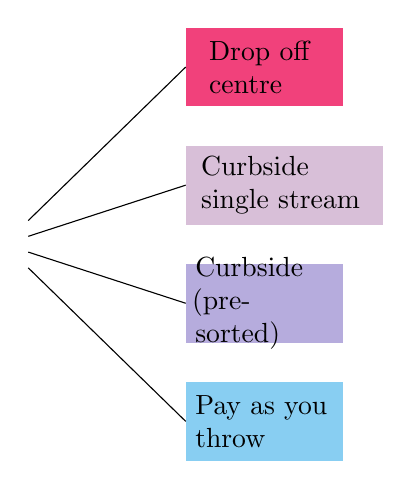
\begin{tikzpicture}
\MindMapOne
%	\fill[color=lime] (0,0) rectangle (4,1) node[pos=.5] {\color{black}``Best'' recycling centre};
%	\fill[color=BurntOrange] (6,2.5) rectangle (8,1.5) node[pos=.5] {\color{black}\begin{minipage}{40pt}\raggedright Most participation\end{minipage}};
%	\fill[color=Goldenrod] (6,0) rectangle (8,1) node[pos=.5] {\color{black}\begin{minipage}{45pt}\raggedright Least cost to the city\end{minipage}};
%	\fill[color=red] (6,-2) rectangle (8,-0.5) node[pos=.5] {\color{black}\begin{minipage}{50pt}\raggedright Processes the most recyclables\end{minipage}};
%	\draw (4,0.75) -- (6,2);
%	\draw (4,0.5) -- (6,0.5);
%	\draw (4,0.25) -- (6,-1.25);
	\fill[color=WildStrawberry!80!white] (10,2.25) rectangle (12,3.25) node[pos=.5] {\color{black}\begin{minipage}{40pt}\raggedright Drop off centre\end{minipage}};	
	\fill[color=Thistle] (10,0.75) rectangle (12.5,1.75) node[pos=.5] {\color{black}\begin{minipage}{60pt}\raggedright Curbside single stream\end{minipage}};	
	\fill[color=Periwinkle!50!white] (10,0.25) rectangle (12,-0.75) node[pos=.5] {\color{black}\begin{minipage}{50pt}\raggedright Curbside (pre-sorted)\end{minipage}};	
	\fill[color=Cerulean!50!white] (10,-2.25) rectangle (12,-1.25) node[pos=.5] {\color{black}\begin{minipage}{50pt}\raggedright Pay as you throw\end{minipage}};
	\draw (8,0.8) -- (10,2.75);	
	\draw (8,0.6) -- (10,1.25);	
	\draw (8,0.4) -- (10,-0.25);	
	\draw (8,0.2) -- (10,-1.75);	
\end{tikzpicture}
\end{center}
\end{example}
\end{siam}

%\begin{figure}[!htbp]
%\begin{tikzpicture}
%	\fill[color=Green] (0,0) rectangle (4,1) node[pos=.5] {\color{black}``Best'' recycling centre};
%	\fill[color=BurntOrange] (6,2.5) rectangle (8,1.5) node[pos=.5] {\color{black}\begin{minipage}{40pt}\raggedright Most participation\end{minipage}};
%	\fill[color=Goldenrod] (6,0) rectangle (8,1) node[pos=.5] {\color{black}\begin{minipage}{45pt}\raggedright Least cost to the city\end{minipage}};
%	\fill[color=red] (6,-2) rectangle (8,-0.5) node[pos=.5] {\color{black}\begin{minipage}{50pt}\raggedright Processes the most recyclables\end{minipage}};
%	\draw (4,0.75) -- (6,2);
%	\draw (4,0.5) -- (6,0.5);
%	\draw (4,0.25) -- (6,-1.25);
%	\fill[color=WildStrawberry] (10,2.25) rectangle (12,3.25) node[pos=.5] {\color{black}\begin{minipage}{40pt}\raggedright Drop off centre\end{minipage}};	
%	\fill[color=Thistle] (10,0.75) rectangle (12.5,1.75) node[pos=.5] {\color{black}\begin{minipage}{60pt}\raggedright Curbside single stream\end{minipage}};	
%	\fill[color=Periwinkle] (10,0.25) rectangle (12,-0.75) node[pos=.5] {\color{black}\begin{minipage}{50pt}\raggedright Curbside (pre-sorted)\end{minipage}};	
%	\fill[color=Cerulean] (10,-2.25) rectangle (12,-1.25) node[pos=.5] {\color{black}\begin{minipage}{50pt}\raggedright Pay as you throw\end{minipage}};
%	\draw (8,0.8) -- (10,2.75);	
%	\draw (8,0.6) -- (10,1.25);	
%	\draw (8,0.4) -- (10,-0.25);	
%	\draw (8,0.2) -- (10,-1.75);	
%\end{tikzpicture}
%\caption{Next step of a mind map.}
%\label{mindmap2}
%\end{figure}


\begin{important}
		There is free online software to help creating a mind map. One such is \href{http://freemind.sourceforge.net}{FreeMind (http://freemind.sourceforge.net)}.
		
		\hfill \qrcode{http://freemind.sourceforge.net}
\end{important}


\begin{graybox}
\begin{minipage}{.75\textwidth}
For more details on creating a mind map, check the book:
\begin{verbatim}
	Math Modeling: Getting Started and Getting Solutions, K. M. Bliss, K. R. Fowler, 
	and B. J. Galluzzo, SIAM, Philadelphia, 2014
\end{verbatim}
\begin{center}
\href{https://m3challenge.siam.org/resources/modeling-handbook}{\tt https://m3challenge.siam.org/resources/modeling-handbook}
\end{center}
\end{minipage}
\hfill
\begin{minipage}{.20\textwidth}
	\hfill\qrcode{https://m3challenge.siam.org/resources/modeling-handbook}	
\end{minipage}
\end{graybox}






	\begin{exercises}
		% Topics:
		% 
	\begin{problist}
		% 
		\prob
		Expand the mind map from the example above by focusing on the other two approaches:
		\begin{enumerate}
			\item Most participation
			\item Processes the most recyclables
		\end{enumerate}

		
	For each part, create a mind map. 
	Focus on the same approach you had for the \hyperref[exercise:define]{questions from the previous module}.

		\prob Help the Canadian Institute of Health Information (CIHI) estimate how significant the outbreak of illnesses will be in the coming year in Canada.
		\prob Create a mathematical model to rank roller coasters according to thrill factor.
		\prob Gas stations offer different prices for gas. I would like to create an app that finds the best gas station to go to. What should ``best'' mean?
		\prob The mayor of Toronto wants to extend the subway line with a new orange line as in \hyperref[p:TTC]{core exercise \ref{p:TTC}}. Is it optimal?
		
		\prob Is it better to buy a car or rent Zipcar, or Car2go?
		
		\prob Help Airbus design the interior of an airplane.

	\end{problist}
\end{exercises}

\end{module}



\begin{lesson}
	\Title{Defining Problem Statement}

	\Heading{Objectives}
	\begin{itemize}
		\item The second step in Mathematical modelling is to construct a representation of how the team will be attempting to solve the problem.
		\item Create a mind map of the problem. This is a structured way to brainstorm possible solutions and their requirements.
	\end{itemize}
	
	\Heading{Motivation} 

\begin{annotation}
	\begin{goals}
	\Goal{Extra Reading}
	Math Modelling: Getting started and getting solutions, Bliss-Fowler-Galluzzo
	
	\hfill \qrcode{https://m3challenge.siam.org/resources/modeling-handbook}	
	\end{goals}
\end{annotation}
	\Heading{Extra Reading} \href{https://m3challenge.siam.org/resources/modeling-handbook}{Math Modelling: Getting started and getting solutions, Bliss-Fowler-Galluzzo}

\end{lesson}




%\newpage


\question
\label{elevatorR}
Consider the elevator problem from question \ref{elevator-define}.


\begin{annotation}
	\begin{notes}
	\begin{itemize}
		\item Students usually come up with more complicated variations:
		\begin{itemize}
			\item Money spent on late employees' salaries
			\item sum of time in minutes that employees are late counting only employees that are at most 15 minutes late
		\end{itemize}
		\item Stick with $T$, a simple first approach
	\end{itemize}	
	\end{notes}
	
\end{annotation}

Your team decides that the mathematical object you will use to show the CEO that you solved or improved the problem is
\begin{itemize}
	\item $T=$ the sum in minutes by which every employee is late.
\end{itemize}

Note that employees that are on time count for 0 minutes (not a negative amount of minutes). \\

Create a mind map for the question: \quad How can $T$ be minimized?


\bookonlynewpage


\question

The city of Toronto decided to tear down the Gardiner expressway. While the demolition is taking place, several key arteries are closed and many intersections are bottled. 
At peak times, a police officer is often posted at this intersection to \emph{optimally} control the traffic lights. 

\begin{parts}
	\item What mathematical meaning can we give to the word optimal in this circumstance? 
	\item Create a mind map for this problem.
\end{parts}




	









\standardonlynewpage


%%%%%%%%%%%%%%%%%%%%%%%%%%%%%%
%
%  MODULE - Making Assumptions
%
%%%%%%%%%%%%%%%%%%%%%%%%%%%%%%



\begin{module}{Making assumptions}
	%\Title{Making Assumptions}
	\label{assumption}

\begin{siam}
	In this module you will learn
\begin{itemize}
	\item that we need to make assumptions to be able to create a model
	\item how to strike a balance between accuracy and solvability
\end{itemize}

\hfill \\




Real problems are complex, so when modelling a real problem mathematically, we must make some assumptions. 

The assumptions that we make will affect the problem we are solving and its difficulty, so we need to strike a balance between:
\begin{itemize}
\item accuracy -- the fewer assumption the better, and
\item solvability -- the more assumptions the better.
\end{itemize}

\begin{annotation}
	\begin{goals}
		When building a mind map, keep track of the assumptions necessary for each step.
	\end{goals}
\end{annotation}

Many assumptions follow naturally when building a mind map. \\


\begin{annotation}
	\begin{goals}
		Remember to justify all your assumptions.
	\end{goals}
\end{annotation}

When figuring which assumption to make, keep in mind the key-factors of the problem and find data when available (usually online). 
If not available, measure data when possible, and if it's not possible, make a reasonable assumption on what the data might look like.

Another thing to keep in mind are \emph{time constraints}. Whether in a class, test, or working in a project, there will be deadlines. Your assumptions should take time constraints into consideration. 



\begin{example}

AN EXAMPLE, PROBABLY BASED ON THE RECYCLING.
	
\end{example}




%\hfill \\

%	\section*{Step D. Parameters or Variables?}\label{D-parvsvar}
%	\addcontentsline{toc}{subsection}{Step D. Parameters or Variables?}
%	
%	
%	
%	When you have defined the problem you want to solve and you have made your (initial) assumptions, it is then time to define some details of the problem.
%	
%	
%	
%	
%	With the problem statement clearly defined and an initial set of assumptions made (a list that will likely get longer), you are ready to start to define the details of your model. Now is the time to pause to ask what
%	is important that you can measure. Identifying these notions as variables, with units and some sense of their range, is key to building the model.
%	The purpose of a model is to predict or quantify something of interest. We refer to these predictions
%	as the outputs of the model. Another term we use
%	for outputs is dependent variables. We will also have independent variables, or inputs to the model. Some quantities in a model might be held constant, in which case they are referred to as model parameters. Let's look at a few simple examples that will help you distinguish between these concepts. We'll also see how they depend on your viewpoint and the problem statement.
%	
%	
%	
%	%There is a clear difference between \emph{variables} and \emph{parameters}. 
%	
%	\begin{definition}[Variables and Parameters]
%	
%	
%	A \emph{variable} represents a model state, and may change during simulation.
%	
%	A \emph{parameter} is commonly used to describe objects statically. A \emph{parameter} is normally a constant in a single simulation, and is changed only when you need to adjust your model behaviour. 
%	\end{definition}
%	
%	%Use a variable instead of a parameter if you need to model some data unit continuously changing over time. Use a parameter instead of a variable if you just need to model some parameter of an object changed only at particular moments of time.
%	
%	
%	
%	\begin{annotation}
%		\begin{goals}
%		\qrcode{https://en.wikipedia.org/wiki/Parameter\#Mathematical\_models}	
%		\end{goals}
%	\end{annotation}
%	\begin{note}{(from Wikipedia)}
%	The quantities appearing in the equations we classify into variables and parameters. The distinction between these is not always clear cut, and it frequently depends on the context in which the variables appear. 
%	
%	Usually a model is designed to explain the relationships that exist among quantities which can be measured independently in an experiment; these are the \emph{variables} of the model. 
%	
%	To formulate these relationships, however, one frequently introduces ``constants'' which stand for inherent properties of nature (or of the materials and equipment used in a given experiment). These are the \emph{parameters}.	
%	\end{note}






%
%
%
%The choice of question in the previous module should determine the \emph{dependent} variable.

%
%The \emph{parameters} are the independent variables in the problem, e.g. the speed of the elevators. The final answer will depend on the parameters in the problem. 
%
%We can estimate the parameters, and sometimes even change them. \\
%
%The \emph{variables} are dependent. This meant that if we change the parameters, the variables will change automatically. 

	\begin{exercises}
		% Topics:
		% 
	\begin{problist}
	\prob
	For each part, you are required to make an estimate for some quantity. Make assumptions and justify them in order to solve the problem.
		\begin{enumerate}
			\item What is the number of piano players in Toronto? \hfill \emph{(Fermi problem)}
			\item How many linear km of roads are there in Toronto?
			\item How much salt the city of Toronto needs for its roads during the Winter?
			\item The skating season in Canada is shortening: What are the key-factors determining its length?
		\end{enumerate}
	\end{problist}
\end{exercises}

\end{siam}
\end{module}
	



\begin{lesson}
	\Title{Making Assumptions}

	\Heading{Objectives}
	\begin{itemize}
		\item The second step in Mathematical modelling is to construct a representation of how the team will be attempting to solve the problem.
		\item Create a mind map of the problem. This is a structured way to brainstorm possible solutions and their requirements.
	\end{itemize}
	
	\Heading{Motivation} 

\begin{annotation}
	\begin{goals}
	\Goal{Extra Reading}
	Math Modelling: Getting started and getting solutions, Bliss-Fowler-Galluzzo
	
	\hfill \qrcode{https://m3challenge.siam.org/resources/modeling-handbook}	
	\end{goals}
\end{annotation}
	\Heading{Extra Reading} \href{https://m3challenge.siam.org/resources/modeling-handbook}{Math Modelling: Getting started and getting solutions, Bliss-Fowler-Galluzzo}

\end{lesson}




%\newpage

\begin{minipage}{.5\textwidth}	
\question
\label{elevator-assumptions}
Consider the elevator problem from \hyperref[elevator-define]{core exercise \ref{elevator-define}}. 


We now give you some technical details about \nobreak{theBigCompany}:

\begin{itemize}
	\item The company occupies the floors 30--33 of the building Place Ville-Marie in Montr\'eal.

	\item Personnel is distributed in the following way: 
	\begin{itemize}
		\item 350 employees in floor 30,
		\item 350 employees in floor 31,
		\item 250 employees in floor 32, 
		\item 150 employees in floor 33.
	\end{itemize}
\end{itemize}

\emph{Note.} Even though these details are fictional, the numbers respect the building code. \\

\emph{Hint.} Focus on a \textbf{few} parameters and variables.
\end{minipage}
\qquad
\begin{minipage}{.5\textwidth}	
\email
\end{minipage}

\begin{parts} 

	\item With your team, decide on what kind of information you would need to have to be able to solve this problem.

	\item Find the relevant information about the elevators (search the internet, by experimentation). Check the reliability of the data you found.

	\item For the relevant information that you cannot obtain, make assumptions. These assumptions should be reasonable and you should be able to justify them.
\end{parts}

\begin{annotation}
	\begin{notes}
		\begin{itemize}
			\item Students usually have trouble starting. 
			\item They usually agree that they have to figure out how elevators work, so you can prompt them to be more specific. 
			
			\item In the end they should come up with questions like these:
			\begin{itemize}
				\item How fast are the elevators?
				\item How much time do elevators take in each floor?
				\item How many floors do elevators stop on their way up?
				\item How many people fit in the elevator?
				\item Should we consider elevator failures?
			\end{itemize}
		\end{itemize}	
	\end{notes}
\end{annotation}




\bookonlynewpage

\hfill

\bookonlynewpage

\question How much would it cost to make a bridge between Toronto and the U.S.?














\standardonlynewpage

%%%%%%%%%%%%%%%%%%%%%%%%%%%%%%
%
%  MODULE - Construction of the Model
%
%%%%%%%%%%%%%%%%%%%%%%%%%%%%%%



\begin{module}{Construct a model}
	%\Title{Construct a model}
	\label{model}

\begin{siam}
	
In this module you will learn
\begin{itemize}
	\item how to build a model based on the previous steps
\end{itemize}

\hfill \\



This is the part of the modelling where we connect all that we have done so far: the problem we defined, the mind map, the assumptions, and all the variables and parameters in a mathematical model to answer the ``mathematical'' problem defined in \hyperref[define]{Step A}.


%When you have defined the problem you want to solve and you have made your (initial) assumptions, it is then time to define some details of the problem.
	
	
With the problem statement clearly defined and an initial set of assumptions made (a list that will likely get longer), you are ready to start to define the details of your model. Now is the time to pause to ask what is important that you can measure. 
Identifying these notions as variables, with units and some sense of their range, is key to building the model.

The purpose of a model is to predict or quantify something of interest. %We refer to these predictions as the outputs of the model. 
	
Creating a model usually means writing down mathematical equations, constructing a graph, analyzing a geometric figure, or do some statistical analysis. \\


\begin{example}
Your team is tasked with finding the best recycling centre (we looked at this example in \hyperref[mindmap]{Step B}) and your  team has chosen to minimize the cost to the city by using drop off centres.

As part of modelling process, your team has made the following assumptions/measurements:
\begin{itemize}
	\item People would be willing to pay \$2.29 to recycle per month or \$0.53 per week
	\item People would make one weekly trip to the centre
	\item Gasoline costs around \$1.26 per litre
	\item On average a passenger car consumes 10 litres per hundred kilometres\\
\end{itemize}

This means that the (one-way) distance people are willing to travel every week to the drop-off centre is
$$
d \;=\; \frac{1}{4.3 \text{ trips/month}} \cdot \frac{\$2.29 / {\text{month}} }{(\$1.26 \text{/L}) \ \cdot\  (0.1 \text{ L / km})} \;=\; 4.2 \text{  km/trip}.
$$

This should help us figure out the best way to place the drop-off centres. \\

The Mathematical model might look like this

\begin{itemize}
	\item Maximize (number of people within a 4.2 km radius of a drop-off centre)
	\item subject to a certain number of drop-off centres (given by the city budget) %\\
\end{itemize}

%\textit{Note. } The model should also include the cost of building a drop off centre.
\end{example}

\begin{graybox}
Assuming that this project was requested for a specific city, the final report should also include some suggested locations for various different budgets.	
\end{graybox}


%\hfill
%
%Sometimes, the mathematical tools necessary to tackle the problem are clear, but often they are not. In those cases it may be helpful to analyze some simple cases.




	\begin{exercises}
		% Topics:
		% 
	\begin{problist}
	\prob
	For each part, create a model to answer the question. Remember all the previous steps.

	\begin{enumerate}
	\item You want to open a piano store in Toronto, where should you open it?
	\item There was a big snow storm in Toronto and the roads need cleaning. How should the city deploy its snow plowers?
	\item The city of Toronto wants to deactivate the Pickering nuclear power plant in favour of renewable power sources. What is the best way to create the same amount of electricity using only renewable sources in the GTA?
	\item Loblaws wants to start an online food delivery service. How should they do it?
	\item The city airport (YTZ) built a tunnel to access the island airport from the city. Before that, they used a ferry. Was building the tunnel a good decision?	
		\end{enumerate}
	\end{problist}
\end{exercises}

\end{siam}

\end{module}



\begin{lesson}
	\Title{Construct a model}

	\Heading{Objectives}
	\begin{itemize}
		\item The second step in Mathematical modelling is to construct a representation of how the team will be attempting to solve the problem.
		\item Create a mind map of the problem. This is a structured way to brainstorm possible solutions and their requirements.
	\end{itemize}
	
	\Heading{Motivation} 

\begin{annotation}
	\begin{goals}
	\Goal{Extra Reading}
	Math Modelling: Getting started and getting solutions, Bliss-Fowler-Galluzzo
	
	\hfill \qrcode{https://m3challenge.siam.org/resources/modeling-handbook}	
	\end{goals}
\end{annotation}
	\Heading{Extra Reading} \href{https://m3challenge.siam.org/resources/modeling-handbook}{Math Modelling: Getting started and getting solutions, Bliss-Fowler-Galluzzo}

\end{lesson}




%\newpage



\begin{minipage}{.5\textwidth}	
\question
Recall the \hyperref[elevator-assumptions]{core exercise \ref{elevator-assumptions}}.

\begin{itemize}
	\item The company occupies the floors 30--33 of the building Place Ville-Marie in Montr\'eal.

	\item Personnel is distributed in the following way: 
	\begin{itemize}
		\item 350 employees in floor 30,
		\item 350 employees in floor 31,
		\item 250 employees in floor 32, 
		\item 150 employees in floor 33.
	\end{itemize}
\end{itemize}

\vspace{2cm}

Write down a mathematical model for this problem.
\label{elevator-model}
\end{minipage}
\qquad
\begin{minipage}{.5\textwidth}	
\email
\end{minipage}

\begin{annotation}
\begin{goals}
	NEED LOTS OF INSTRUCTIONS FOR INSTRUCTORS HERE!
\end{goals}	
\end{annotation}


















\standardonlynewpage


%%%%%%%%%%%%%%%%%%%%%%%%%%%%%%
%
%  MODULE - Model Assessment
%
%%%%%%%%%%%%%%%%%%%%%%%%%%%%%%



\begin{module}{Model Assessment}
	%\Title{Model Assessment}
	\label{analysis}

\begin{siam}
	
In this module you will learn
\begin{itemize}
	\item how to analyze a model
	\item to check the quality of the model
\end{itemize}

\hfill \\



At this point, you have defined a problem statement, and a mind map to help you decide how to approach the problem. You have made assumptions and made note of them and justified them.
You finally created a model to solve the problem.

The next step is to analyze the model.

There are two types of analysis:


\paragraph{\textcolor{cyan}{\textbf{Superficial assessment.}}} Are the units correct? Are the variables and parameters of a reasonable magnitude? Does it behave as expected? Does it make sense?



\paragraph{\textcolor{cyan}{\textbf{In-depth assessment.}}} Once the superficial assessment is verified, we need to understand the model at a deeper level. 

What are the model's strengths? What are its weaknesses?

When you change the inputs of the model, how do the outputs change? This is called {\emph sensitivity analysis}. 


%Next is a simple example adapted from \cite{bliss}.


%\begin{annotation}
%	\begin{goals}
%	\Goal{Desmos Graph}
%	\hfill \qrvideo{https://www.desmos.com/calculator/z9cftzus0z}
%	\end{goals}
%\end{annotation}

\begin{example}\textbf{Modelling the flu}

History of the project:
\begin{itemize}
	\item Split population into two classes: \emph{infected} and \emph{not infected}
	\item Assume that each infected person infects $R$ number of non infected people every $b$ days
	\item Define $I(n) = $ number of infected people after $n$ days
	\item The two previous points imply \quad $I(n + b) = I(n) + R \, I(n)$
	\item We can then conclude that \quad $I(n b) = (1+R)^n \, I(0)$ \hfill (why?) \\
\end{itemize}

After plotting the resulting function $I(n)$ (with $R=5, b=2, I(0)=20$), we can assess our model.
\begin{center}
	\includegraphics*[width=300pt]{images/module5-graph.png}	
\end{center}
\begin{itemize}
	\item \qrvideo{https://www.desmos.com/calculator/deh5qeea20}
\end{itemize}


\emph{Strengths:}
\begin{itemize}
	\item After two days $(b=2)$, there are 6 infected people, so it is following our assumption
	\item The number of infected people increases faster and faster as expected 
	\item The disease spreads at a constant rate. Also on Desmos, check the infection rate $\dfrac{I(n+b)}{I(n)}$
	\item We could find an explicit formula for the number of infected individuals $I(n)$ \\
\end{itemize}


\emph{Weaknesses:}
\begin{itemize}
	\item The model is too simple, so it doesn't model the spread of the flu accurately
	\item The model yields an exponential rate of infection, which is not possible for very long
	\item The model predicts that eventually the disease will spread to everyone
	\item The model assumes that there are only two types of people: infected and susceptible. Do people recover from the disease?
\end{itemize}

\end{example}




After assessing the model, if time allows, it is important to re-think the model and the assumptions made.



	\begin{exercises}
		% Topics:
		% 
	\begin{problist}
	\prob
	Assess the models created in question \ref{models1}:

	\begin{enumerate}
		\item You want to open a piano store in Toronto, where should you open it?
		\item There was a big snow storm in Toronto and the roads need cleaning. How should the city deploy its snow plowers?
		\item The city of Toronto wants to deactivate the Pickering nuclear power plant in favour of renewable power sources. What is the best way to create the same amount of electricity using only renewable sources in the GTA?
		\item Loblaws wants to start an online food delivery service. How should they do it?
		\item The city airport (YTZ) built a tunnel to access the island airport from the city. Before that, they used a ferry. Was building the tunnel a good decision?	
	\end{enumerate}
	\end{problist}
\end{exercises}

\end{siam}

\end{module}



\begin{lesson}
	\Title{Model Assessment}

	\Heading{Objectives}
	\begin{itemize}
		\item The second step in Mathematical modelling is to construct a representation of how the team will be attempting to solve the problem.
		\item Create a mind map of the problem. This is a structured way to brainstorm possible solutions and their requirements.
	\end{itemize}
	
	\Heading{Motivation} 

\begin{annotation}
	\begin{goals}
	\Goal{Extra Reading}
	Math Modelling: Getting started and getting solutions, Bliss-Fowler-Galluzzo
	
	\hfill \qrcode{https://m3challenge.siam.org/resources/modeling-handbook}	
	\end{goals}
\end{annotation}
	\Heading{Extra Reading} \href{https://m3challenge.siam.org/resources/modeling-handbook}{Math Modelling: Getting started and getting solutions, Bliss-Fowler-Galluzzo}

\end{lesson}




%\newpage

\question

Continuing on the \hyperref[elevator-model]{elevator problem}, let us think of this model for the problem.

\textbf{Facts:}
\begin{itemize}
	\item Loading time of people at ground floor = 20 s
	\item Speed of uninterrupted ascent/descent = 1.5 floors/s
	\item Stop time at a floor = 7 s
	\item Number of elevators serving floors 30--33 = 8

	(these elevators serve floors 23-33 = 11 floors)
	
	\item Maximal capacity of elevators = 25 people
\end{itemize}


\textbf{Assumptions:}
\begin{itemize}
	\item Personnel that should start at time $t$, arrive uniformly in the interval $[t-30, t-5]$ in minutes
	\item First arrived, first served
	\item During morning rush hour, elevators don't stop on the way down
	\item Elevators stop only at half the floors they serve
	\item Elevator failures are neglected
	\item Mean number of people per floor is equal to the mean number of people per floor of the BigCompany
	\item Elevators are filled, in average, to 80\% of their capacity
\end{itemize}


\textbf{Model:}
\begin{itemize}
	\item Mean number of people per floor $= d = \dfrac{350+350+250+150}{4} = 275$ people / floor
	\item Number of people on floors served by elevators (11 floors) $= N = d \cdot 11 = 3025$ people
	\item Time $\Delta t$ of one trip

\hfil $\Delta t \quad = \quad $ \framebox{$\substack{\text{loading time on}\\\text{ground floor}}$} 
		$ \;+ \;$ \framebox{$\substack{\text{time of flight}\\\text{ground $\to 33$}}$}
		$ \;+\; $ \framebox{$\substack{\text{time of flight}\\\text{$33 \to$ ground}}$}
		$\;+\; $ \framebox{$\substack{\text{stop time to}\\\text{6 of the 11 floors}}$} $\quad = \quad$ 106 s
		
		\item Number of trips necessary per elevator $= n = \dfrac{3025}{20 \cdot 8} \approx 19$ trips

		\item Time necessary to carry the staff of the BigCompany $= \pmb{t} = \dfrac{19 \cdot 106}{60} = 33 $ minutes
		
		\item Accumulated late time $ = \pmb{T} = 180 \cdot 20 \cdot 8 + 74 \cdot 20 \cdot 8 = 40\,640$ seconds $= $ 11h18m

\end{itemize}

\hfill

\begin{annotation}
	\begin{notes}

Some questions to guide the students:
	\begin{itemize}
	\item What are the strengths?
	\item What are the weaknesses?
	\item Is the result around what you expected?
\end{itemize}	
	
\hfill \\
In case students don't realize that something is wrong:
\begin{itemize}
	\item People start arriving 30 minutes before the starting time, so \emph{almost everybody will be on time?}
	\item Assume that the CEO of the BigCompany is right: people are arriving late! What's wrong with the model?

	\item Which assumptions should be relaxed? Or checked?
	\item If one needs to be replaced, by what?
	\end{itemize}
	
	\end{notes}
\end{annotation}

Your task is to assess this model.
Be ready to report on your assessment.



















\standardonlynewpage


%%%%%%%%%%%%%%%%%%%%%%%%%%%%%%
%
%  MODULE - Report
%
%%%%%%%%%%%%%%%%%%%%%%%%%%%%%%



\begin{module}{Putting it all together}
	%\Title{Putting it all together}
	\label{report}

	\begin{siam}
In this module you will learn
\begin{itemize}
	\item how to put all that you have done together into a well structured report
\end{itemize}

\hfill \\



This is the final stage of the modelling project.

By now, you have started with a mathematically defined problem, with some assumptions, and you have created a mind map to help you navigate the problem.
You have also constructed a model and assessed it to make sure it is sound.

All that we have left is to put all this work together into the form of a report.



The report should consist of two parts:

\begin{enumerate}
	\item \textbf{Summary. } Should be at most one page long, and contain a statement of the problem, a brief description of the methods chose to solve it, and some final results and a conclusion. In this part of the report, you should keep mathematical symbols to a minimum, so the reader gets an idea of what to expect in the remainder of the report without getting bogged down in unfamiliar mathematics.

	\item \textbf{In-depth report. } This is where the details go in. It should start with an introduction to the problem assuming that the reader is not aware of it. It should then be structured according to the steps we did before:
	\begin{itemize}
		\item Optionally, you can include a mind map with a description of how it guided the whole process
		\item Assumptions and variables in the model
		\item The model described in detail
		\item The solution process
		\item The assessment of the model
		\item A conclusion, with a description of the results
	\end{itemize}
\end{enumerate}





\begin{example}
As an example of an excellent report, please read the report from the winning team of the 2019 $M_3C$ challenge:
\begin{itemize}
	\item \qrvideo{https://uoft.me/modelling-app-report}
	\item Read the summary and chapters 1, 2, 5.
\end{itemize}
\end{example}

\end{siam}

\begin{siam2019}


\begin{definition}[Report checklist]

\begin{tabular}{|p{75pt}|p{200pt}|p{125pt}|}
\hline
\textbf{Component}
	& \textbf{Questions about your model and how you made it}
	& \textbf{Useful vocabulary} \\ \hline
\multirow{2}{75pt}[-10pt]{\textbf{Defining the problem}}
	& What is/are the big problem/s that you have been asked to solve?
		& open-ended problem \\ \cline{2-3}
	& What is the specific problem your model is going to solve?
		& specific, focus \\ \hline
\multirow{4}{75pt}[-25pt]{\textbf{Making assumptions}}
	& What ideas did you think about that you decided not to try? 
		& eliminate, prioritize \\ \cline{2-3}
	& What have you assumed in order to solve the problem? Why did you make these choices? 
		& assumption, constraints \\ \cline{2-3} %\hline
%\multirow{2}{75pt}{\textbf{Defining variables}}
	& What quantities are important? Which ones change and which ones stay the same? 
		& variable  \\ \cline{2-3}
	& Where did you find the numbers that you used in your model? 
		& resources, citations \\ \hline
\multirow{2}{75pt}[-15pt]{\textbf{Getting a solution}}
	& What pictures, diagrams or graphs might help people understand your information, model, and results? 
		& diagram, graph, labels  \\ \cline{2-3}
	& What mathematical ideas did you use to describe the situation and solve your problem? 
		& situation  \\ \hline
\multirow{4}{75pt}[-30pt]{\textbf{Model assessment}}
	& How do you know that your calculations are correct? Did you remember to use units (like dollars or metres?) 
		& calculation, unit \\ \cline{2-3}
	& When does your model work? When do you need to be careful because it might not? 
		& limitations  \\ \cline{2-3}
	& How do you know you have a good/useful model? Why does your model make sense? 
		& testing, validation \\ \cline{2-3}
	& If you were going to make your model better, what would you do? 
		& improvement, iteration \\ \hline
\multirow{3}{75pt}[-20pt]{\textbf{Reporting results}}
	& Explain your mathematical model in words and math. 
		& clarity, concision \\ \cline{2-3}
	& What are the strengths and weaknesses of your model?
		& strengths, weaknesses \\ \cline{2-3}
	& What are the 5 most important things for your audience/client to understand about your model and/or solution? 
		& client, audience \\ \hline
\end{tabular}

\hfill \\

This checklist is adapted from

\begin{graybox}
\begin{minipage}{.75\textwidth}
\begin{verbatim}
	GAIMME: Guidelines for Assessment and Instruction in Mathematical
	Modeling Education, Second Edition, Sol Garfunkel and Michelle
	Montgomery, editors, COMAP and SIAM, Philadelphia (2019)
\end{verbatim}
\begin{center}
\url{https://uoft.me/gaimme}
\end{center}
\end{minipage}
\hfill
\begin{minipage}{.20\textwidth}
	\hfill\qrcode{https://uoft.me/gaimme}	
\end{minipage}
\end{graybox}

\end{definition}

	
\end{siam2019}




	\begin{noexercises}

%	\begin{problist}
%	\prob
%	Reports!
%
%	\end{problist}
\end{noexercises}

\end{module}



\begin{lesson}
	\Title{Putting it all together}

	\Heading{Objectives}
	\begin{itemize}
		\item The second step in Mathematical modelling is to construct a representation of how the team will be attempting to solve the problem.
		\item Create a mind map of the problem. This is a structured way to brainstorm possible solutions and their requirements.
	\end{itemize}
	
	\Heading{Motivation} 

\begin{annotation}
	\begin{goals}
	\Goal{Extra Reading}
	Math Modelling: Getting started and getting solutions, Bliss-Fowler-Galluzzo
	
	\hfill \qrcode{https://m3challenge.siam.org/resources/modeling-handbook}	
	\end{goals}
\end{annotation}
	\Heading{Extra Reading} \href{https://m3challenge.siam.org/resources/modeling-handbook}{Math Modelling: Getting started and getting solutions, Bliss-Fowler-Galluzzo}

\end{lesson}







%\newpage

%\question
%Another question to be added here
%
%\newpage





%
%
%
%
%\begin{module}
%	\Title{Putting it all together}
%	\Heading{Textbook} \href{https://m3challenge.siam.org/resources/modeling-handbook}{Math Modelling: Getting started and getting solutions, Bliss-Fowler-Galluzzo}
%	
%	\Heading{Objectives}
%	\begin{itemize}
%		\item Bla bla bla	
%	\end{itemize}
%	
%	\Heading{Motivation} 
%
%
%\end{module}
%
%
%
%
%\section*{Step F. Writing a report}\label{F-report}
%\addcontentsline{toc}{subsection}{Step F. Writing a report}
%









%%%%%%%%%%%%%%%%%%%%%%%%%%%%%%%%%%%%%%%%%%%%%%%%%%%%%%%%%%%%%%%%%%%%%%%%
%
%		Chapter 1 - Introduction to Differential Equations
%
%%%%%%%%%%%%%%%%%%%%%%%%%%%%%%%%%%%%%%%%%%%%%%%%%%%%%%%%%%%%%%%%%%%%%%%%





%%%%%%%%%%%%%%%%%%%%%%%%%%%%%%%%%%%%%%%%%%%%%%%%%%%%%%%%%%%%%%%%%%%%%%%%
%
%		Chapter 1 - Introduction to ODEs
%
%%%%%%%%%%%%%%%%%%%%%%%%%%%%%%%%%%%%%%%%%%%%%%%%%%%%%%%%%%%%%%%%%%%%%%%%


\begin{topic}[Introduction to Differential Equations]

\end{topic}




%%%%%%%%%%%%%%%%%%%%%%%%%%%%%%%%%%%%%%%%%%%%%%%%%%%%%%%%%%%%%%%%%%%%%%%%
%		Definitions


\begin{module}{Definition}
%	\Title{Definitions}
	\Heading{Textbook}	
	\Heading{Objectives}
	\begin{itemize}
		\item Bla bla bla	
	\end{itemize}
	
	\Heading{Motivation} 


\end{module}


















\newpage


%%%%%%%%%%%%%%%%%%%%%%%%%%%%%%
%
%  MODULE - Solutions
%
%%%%%%%%%%%%%%%%%%%%%%%%%%%%%%



\begin{module}{Solutions}
	%\Title{Solutions}
	\label{intro-sols}

	In this module you will learn
\begin{itemize}
	\item what is a solution of a differential equation
	\item the difference between a solution and an integral curve
\end{itemize}

\hfill \\[-10pt]

Assume that we have found a differential equation that models a situation.
Often the goal is to figure out what happens, so we usually attempt to either solve the differential equation and obtain a solution or to find an approximation for the solution.

In this module, we will discuss solutions in more detail.

\begin{definition}[Solution]
	Given a differential equation, a \emph{solution} is a differentiable function that satisfies the differential equation.
\end{definition}

\begin{example}
Consider the differential equation
$$
t \frac{du}{dt} = u + t^2 \cos(t).
$$

Then the function 
$$
u(t) = t\sin(t)
$$
is a solution, because
$$
t \frac{du}{dt} = t \big( \sin(t) + t \cos(t) \big) = t \sin(t) + t^2 \cos (t) = u + t^2 \cos(t).
$$
\end{example}



\begin{definition}[Integral curve]
	We can represent all the solutions geometrically as an infinite family of curves. These curves are called \emph{integral curves}.
\end{definition}

\begin{example}\label{sols-ex}
Consider the initial-value problem
$$
\begin{cases}
	\dfrac{dy}{dx}=-\dfrac{x}{y} \\
	y(0)=-3
\end{cases}
$$
Then, we can check that curves of the form $x^2 + y^2 = C$ satisfy this differential equation.

This gives us the solution
$$
y(x) = - \sqrt{9 - x^2}.
$$

However, the integral curve for this initial-value problem is the curve
$$
x^2 + y^2 = 9
$$


\begin{center}
\begin{tabular}{cc}
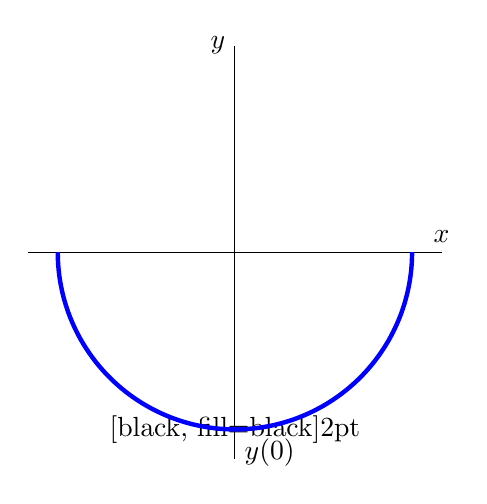
\begin{tikzpicture}[xscale=0.75,yscale=0.75]
	\draw[-{\seta}] (-3.5,0) -- (3.5,0) node[above] {$x$};
	\draw[-{\seta}] (0,-3.5) -- (0,3.5) node[left] {$y$};
	\draw[] (0,-3) node {\tikzcircle[black, fill=black]{2pt}};
	\draw[] (0,-3) node[below right] {$y(0)$};
  \draw[samples=100,ultra thick,domain=0:180,smooth,variable=\t,blue] plot ({3*cos(\t)},{-3*sin(\t)});
\end{tikzpicture}
	& 
	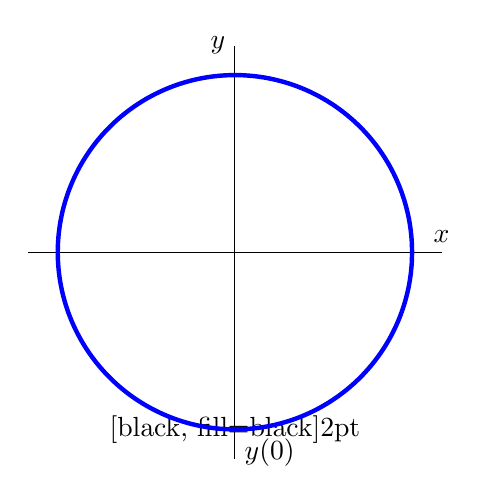
\begin{tikzpicture}[xscale=0.75,yscale=0.75]
		\draw[-{\seta}] (-3.5,0) -- (3.5,0) node[above] {$x$};
		\draw[-{\seta}] (0,-3.5) -- (0,3.5) node[left] {$y$};
		\draw[] (0,-3) node {\tikzcircle[black, fill=black]{2pt}};
		\draw[] (0,-3) node[below right] {$y(0)$};
	  \draw[samples=100,ultra thick,domain=0:360,smooth,variable=\t,blue] plot ({3*cos(\t)},{-3*sin(\t)});
	\end{tikzpicture}

	\\
Solution of the initial-value problem
	& Integral curve for the initial-value problem
\end{tabular}
\end{center}





\end{example}



	\begin{exercises}
		% Topics:
		% 
	\begin{problist}
	\prob Check that curves of the form $x^2 + y^2 = C$ satisfy the differential equation $\dfrac{dy}{dx} = -\dfrac{x}{y}$.
	
	
	\prob Is the piecewise-defined function
	$$
	y(x) = \begin{cases}
 		-x^2 & \text{ if } x< 0 \\
 		x^2 & \text{ if } x \geq 0		
	\end{cases}
	$$
	a solution of the differential equation $xy'-2y=0$ on $(-\infty,\infty)$?
	
	
	\prob Consider the differential equation
	$$ y^{(4)} - 8y^{3)} + 26 y'' - 40y'+25y=0.$$
	
	\begin{enumerate}
		\item Is $y=4 e^{2x}\sin(x)$ a solution?
		\item Is $y=-8 x e^{2x}\cos(x)$ a solution?
		\item For the two function above, if they are solutions, what are initial conditions of the form
			\begin{itemize}
				 \item[] $y(0) =$
				 \item[] $y'(0) =$
				 \item[] $y''(0) =$
				 \item[] $y'''(0) =$
			\end{itemize}
			that the solution satisfies?
	\end{enumerate}


	\prob Consider the functions
	\begin{align*}
		f(x) & = 3x + x^2 	& g(x) & = e^{-7x} \\
		h(x) & = \sin(x) 	& j(x) & = \sqrt{x} \\
		k(x) & = 8 e^{3x}	& \ell(x) & = -2 \cos(x)
	\end{align*}
	
	Match each differential to one or more functions which are solutions.
	
	\begin{enumerate}
		\item $y'=3y$
		\item $y''+9y'+14y=0$
		\item $y''+y=0$
		\item $2x^2y'' + 3xy'=y$
	\end{enumerate}
	
	
	
	\prob Consider the differential equation $u' = -2(u-10)$.
	
	\begin{enumerate}
		\item Check that the curves of the form $u = 10 + C e^{-2t}$ satisfy the differential equation.
		\item Sketch one solution of the differential equation.
		\item Sketch all the integral curves for the differential equation.
		\item What is the difference between a solution passing through the point $(1,20)$ and an integral curve passing through the same point?
	\end{enumerate}


	\prob Consider the differential equation $y'\big( 3y^2-1\big) = 1$.
	
	\begin{enumerate}
		\item Check that the curves of the form $y^3-y=x+C$ satisfy the differential equation.
		\item Sketch the solution of the differential equation that passes through $(1,1)$.
		\item Sketch the integral curve for the differential equation that passes through $(1,1)$.
		\item What is the difference between a solution passing through the point $(1,1)$ and an integral curve passing through the same point?
		\item Repeat (b)--(d) with the points $(1,0)$ and $(1,-1)$ instead of $(1,1)$.
	\end{enumerate}


	\prob Consider the ODE \quad $y'(t) = \big(y(t)\big)^2$ \quad .
	One of these two graphs {\bf cannot} describe the solution. 
	Which one? 
	
	
	\begin{center}
	\begin{tikzpicture}
		\draw[-{\seta}] (-1,0) -- (3,0) node[above] {$t$};
		\draw[-{\seta}] (0,-3) -- (0,1) node[left] {$y$};
		\draw[ultra thick,domain=0.5:2.5,smooth,variable=\x,blue] plot ({\x},{(\x*\x-5)/3-1});
	\end{tikzpicture}
	\hfil
	\begin{tikzpicture}
		\draw[-{\seta}] (-1,0) -- (3,0) node[above] {$t$};
		\draw[-{\seta}] (0,-3) -- (0,1) node[left] {$y$};
		\draw[ultra thick,domain=0.5:2.5,smooth,variable=\x,blue] plot ({\x},{-((\x-3.5)^2)/4-0.25});
	\end{tikzpicture}	
	\end{center}

	\prob We seek a first-order ordinary differential equation \quad $y' = f(\pmb{y})$ \quad whose solutions satisfy
	$$
	\begin{cases}
	y(x)  \mbox{ is concave up if } y < 1 \\
	y(x) \mbox{ is concave down if } y > 1
	\end{cases}
	$$
	%
	Write down or graph a function $f(y)$ that would produce such solutions.

	
	\end{problist}
\end{exercises}

\end{module}



\begin{lesson}
	\Title{Solutions}

	\Heading{Objectives}
	\begin{itemize}
		\item The second step in Mathematical modelling is to construct a representation of how the team will be attempting to solve the problem.
		\item Create a mind map of the problem. This is a structured way to brainstorm possible solutions and their requirements.
	\end{itemize}
	
	\Heading{Motivation} 

\begin{annotation}
	\begin{goals}
	\Goal{Extra Reading}
	Math Modelling: Getting started and getting solutions, Bliss-Fowler-Galluzzo
	
	\hfill \qrcode{https://m3challenge.siam.org/resources/modeling-handbook}	
	\end{goals}
\end{annotation}
	\Heading{Extra Reading} \href{https://m3challenge.siam.org/resources/modeling-handbook}{Math Modelling: Getting started and getting solutions, Bliss-Fowler-Galluzzo}

\end{lesson}




\newpage

\question

Which of these shows solutions of $y' = (x-1)(x+1) = x^2 - 1$ ?

\newlength{\len}
\setlength{\len}{120pt}
\begin{tabular}{ccc}
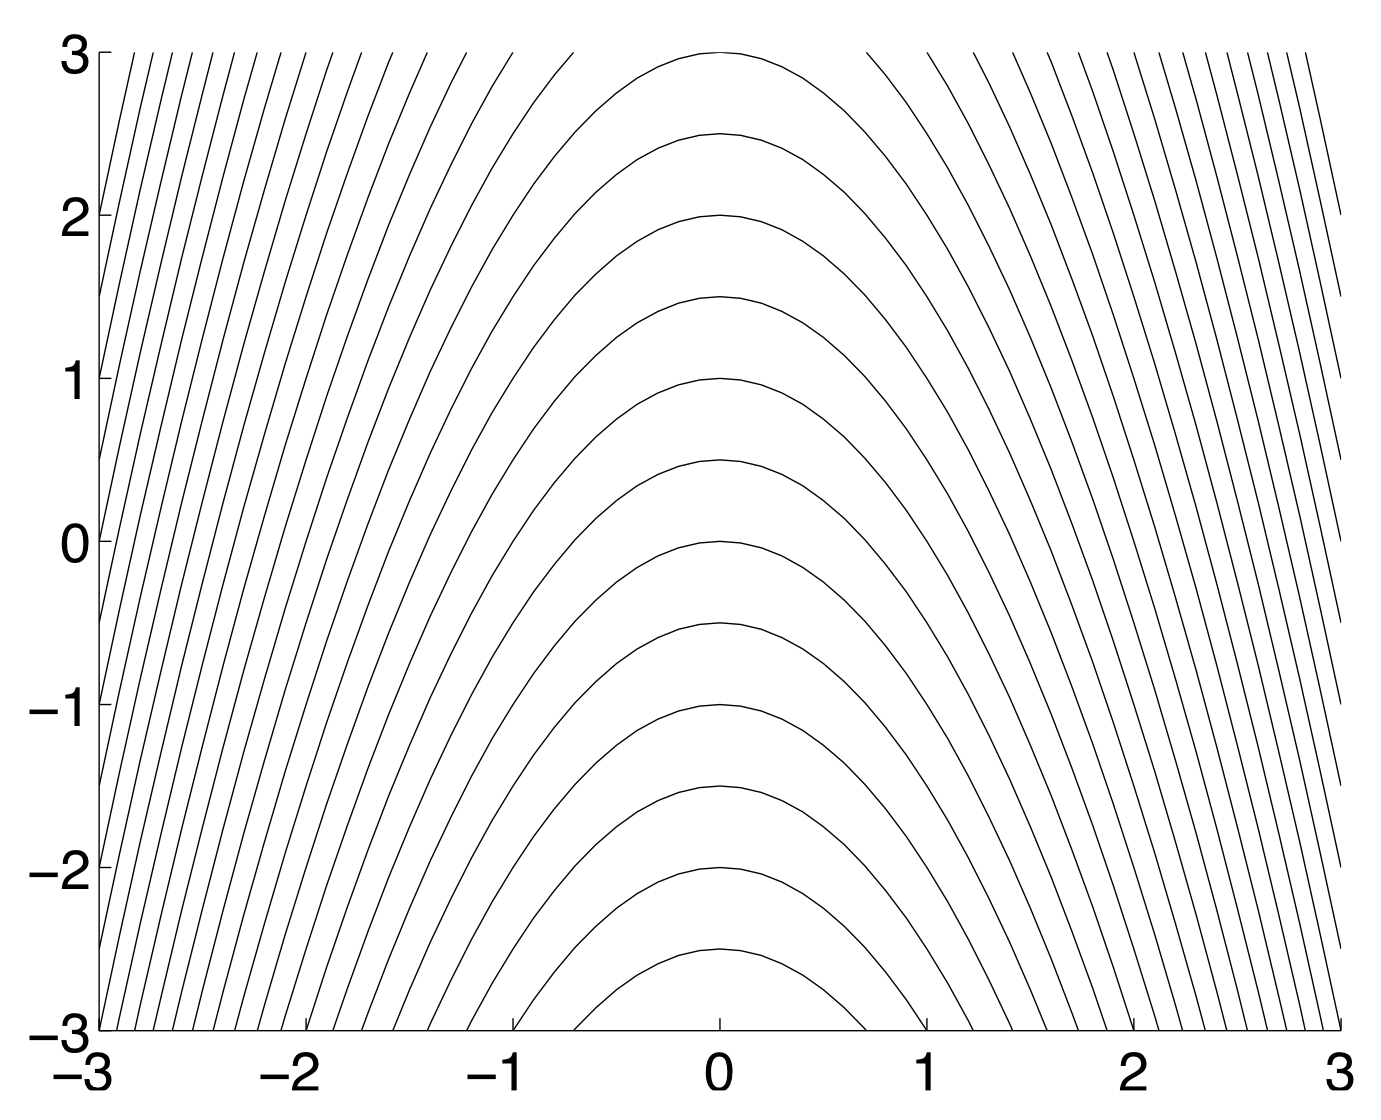
\includegraphics[width=\len]{images/module8-figs-6.png}
	& 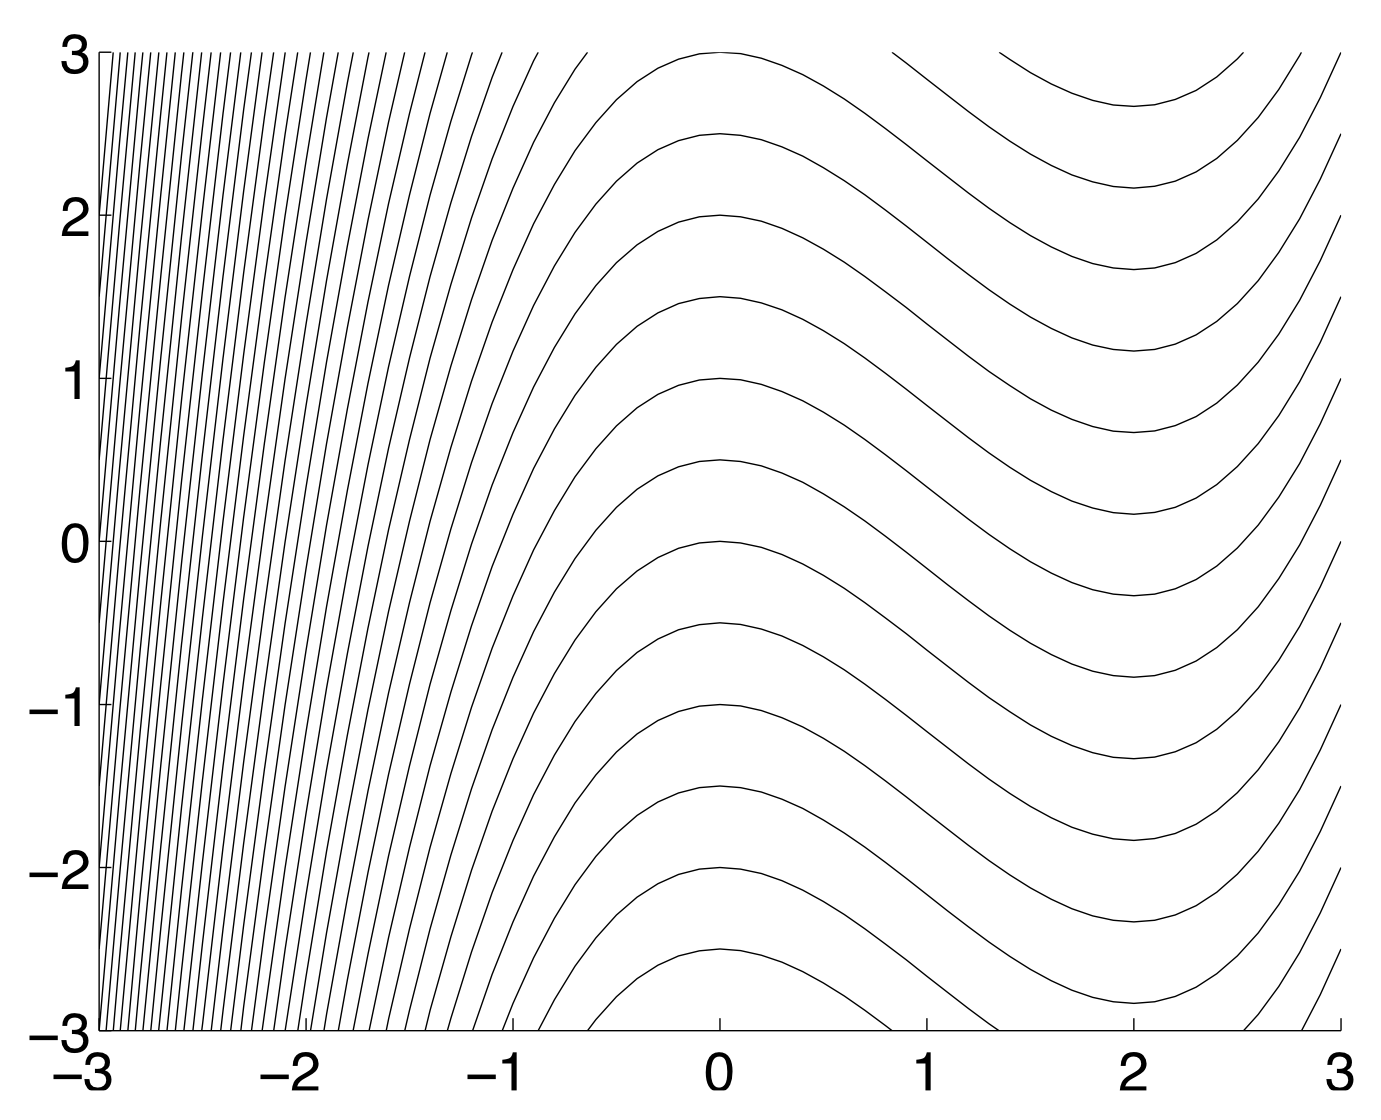
\includegraphics[width=\len]{images/module8-figs-3.png}
	& \includegraphics[width=\len, page=2]{images/module8-figs-2.png} \\
A & B & C \\[15pt]
%
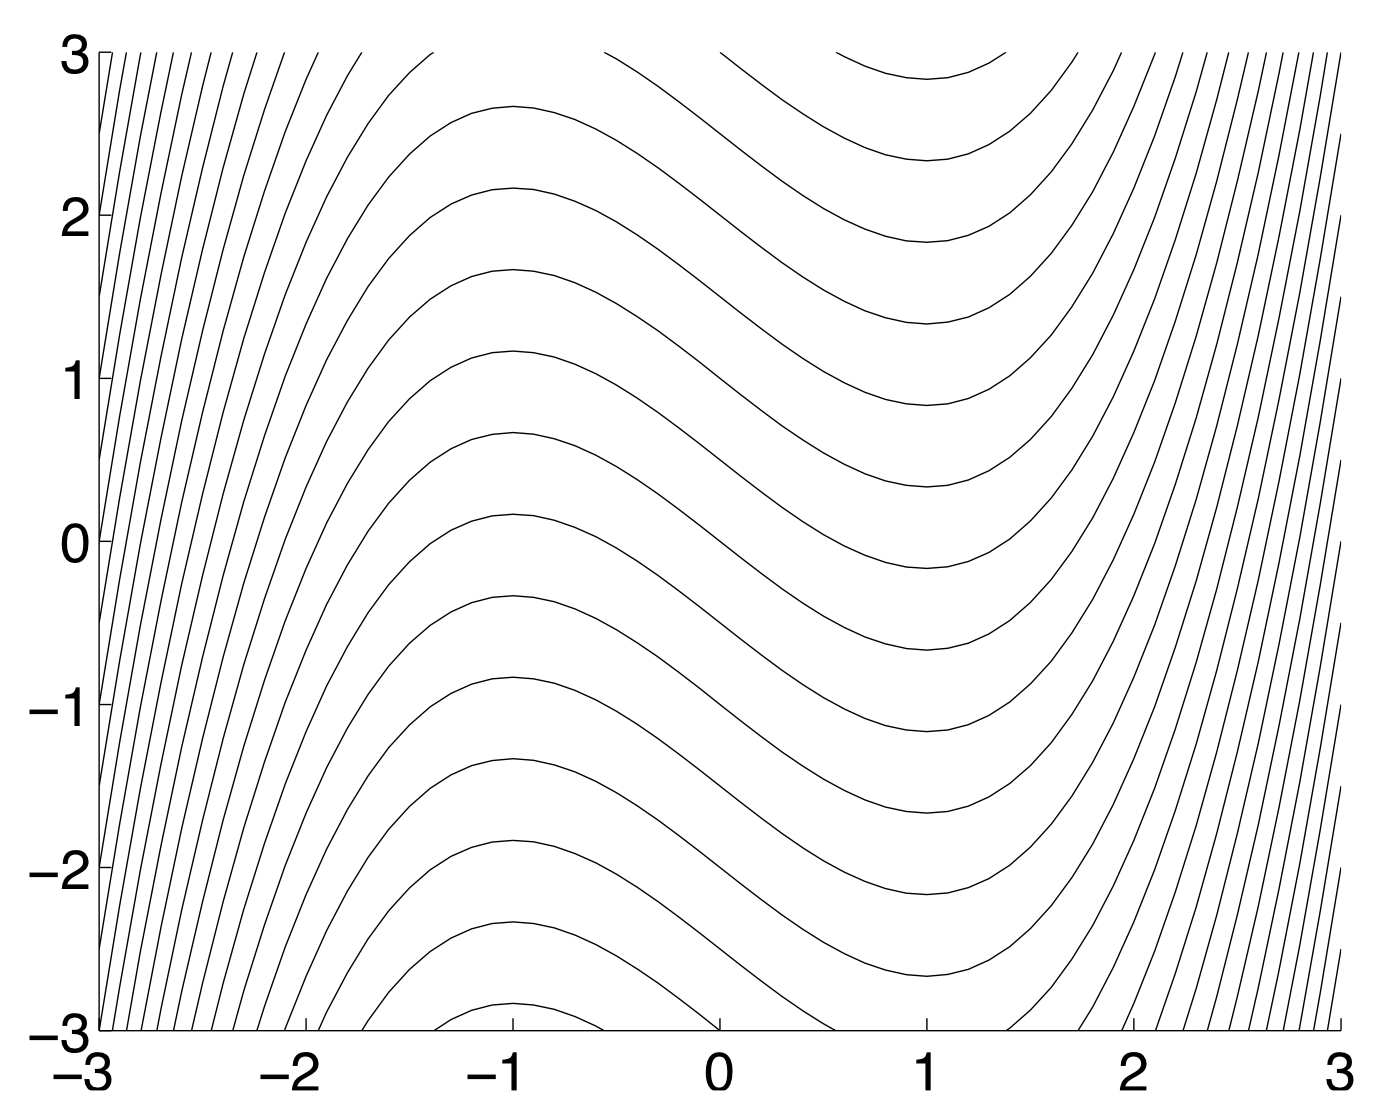
\includegraphics[width=\len]{images/module8-figs-1.png}
	& 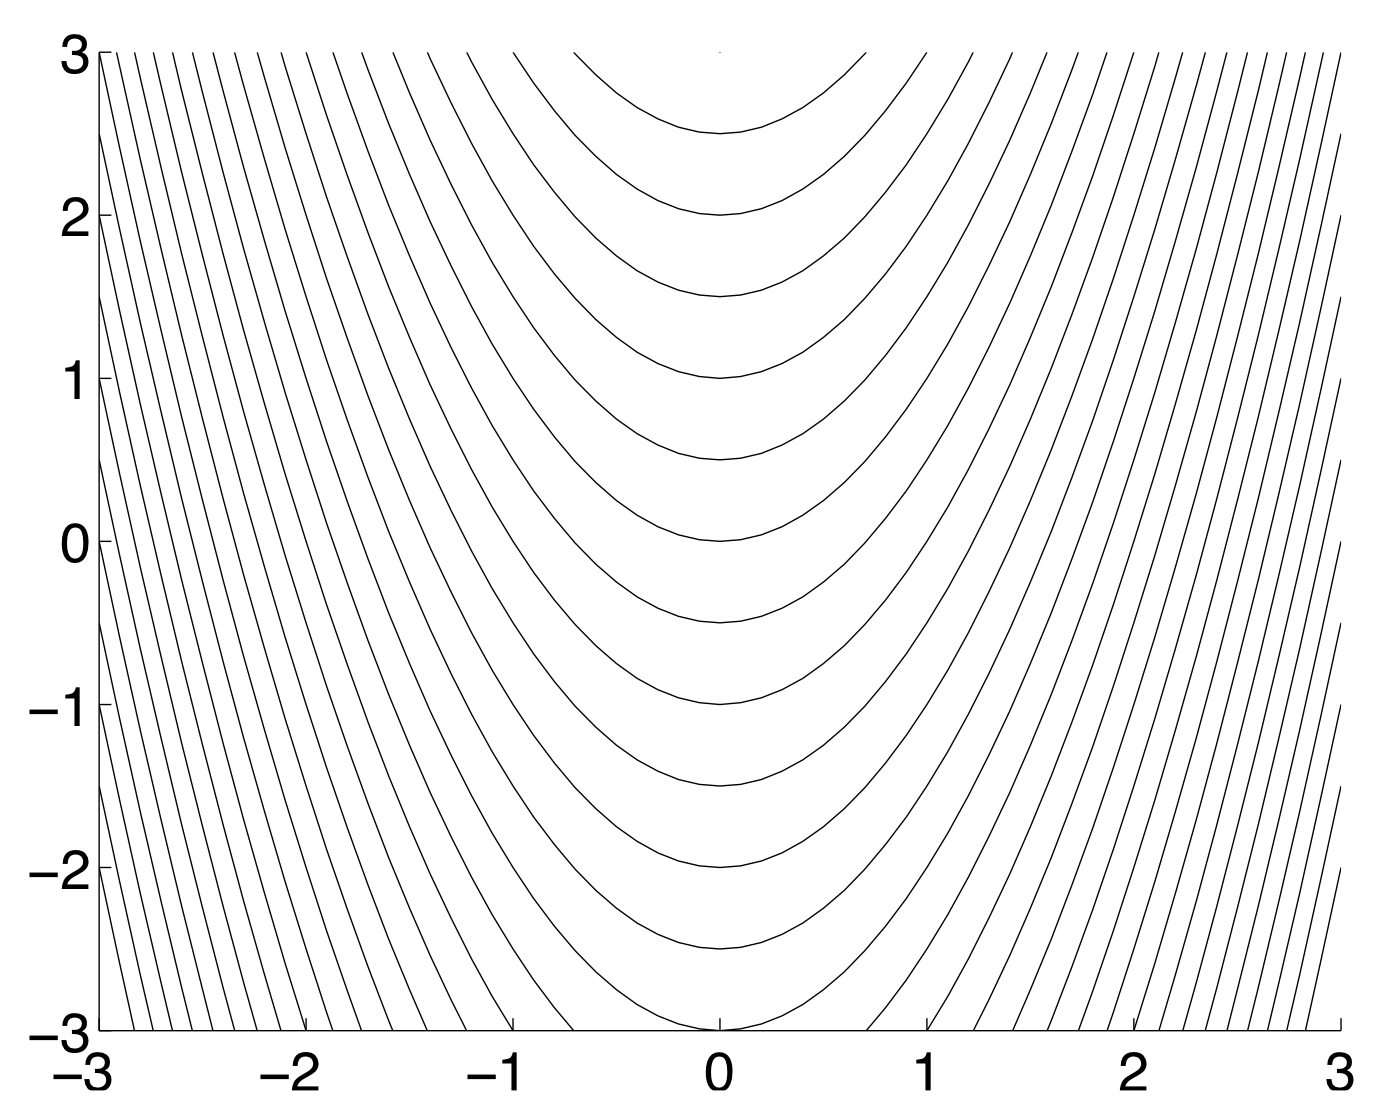
\includegraphics[width=\len]{images/module8-figs-5.png}
	& 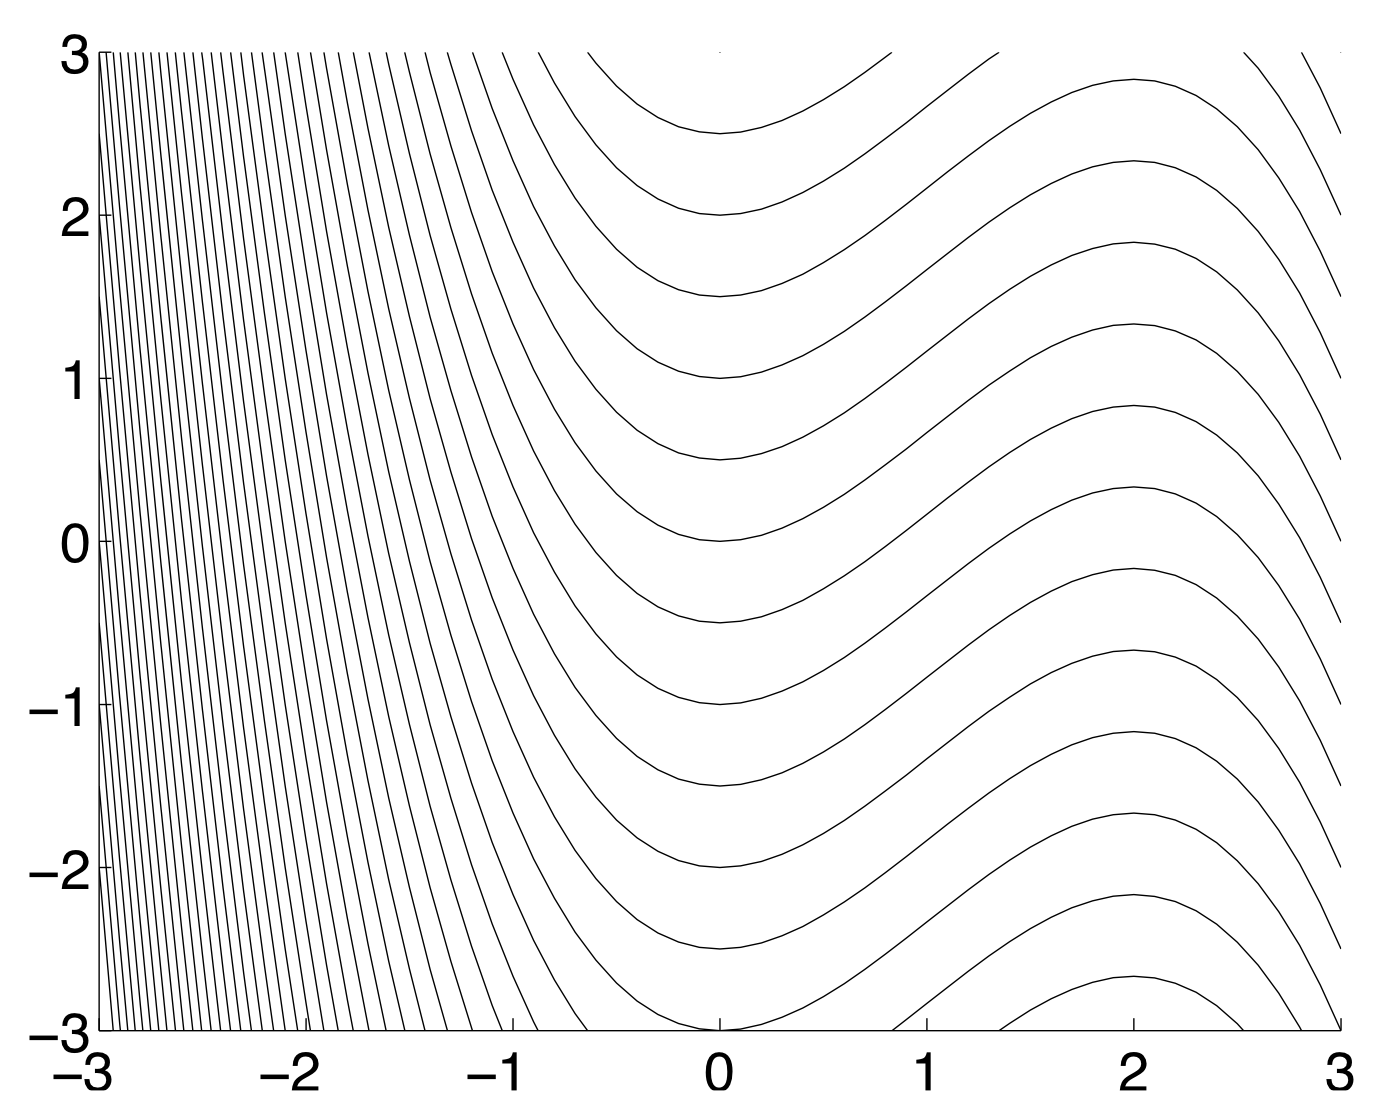
\includegraphics[width=\len]{images/module8-figs-4.png} \\
D & E & F \\
\end{tabular}

%		\begin{tabular}{ccc}
%		%	\begin{tikzpicture}
%		%	    \begin{scope}
%		%	    \clip (-3,-3) rectangle (3,3);
%		%		\foreach \k in {-9,-8, ..., 36} {
%		%	      \draw[samples=50,domain=-3:3,variable=\x] plot ({\x},{\k/3-(\x*\x)});
%		%	    }
%		%	    \end{scope}
%		%	    \draw[thick] (-3,-3) -- (-3,3);
%		%	    \draw[thick] (-3,-3) -- (3,-3);
%		%	    \foreach \k in {-3,-2, ..., 3} {
%		%	      \draw ({\k,-3}) node[below] {\tiny $\k$};
%		%	      \draw ({-3,\k}) node[left] {\tiny $\k$};
%		%	    }
%		%	\end{tikzpicture}
%		\includegraphics[width=\len, page=6]{images/module8-figs.pdf}
%			& \includegraphics[width=\len, page=3]{images/module8-figs.pdf}
%			& \includegraphics[width=\len, page=2]{images/module8-figs.pdf} \\
%		A & B & C \\[15pt]
%		%
%		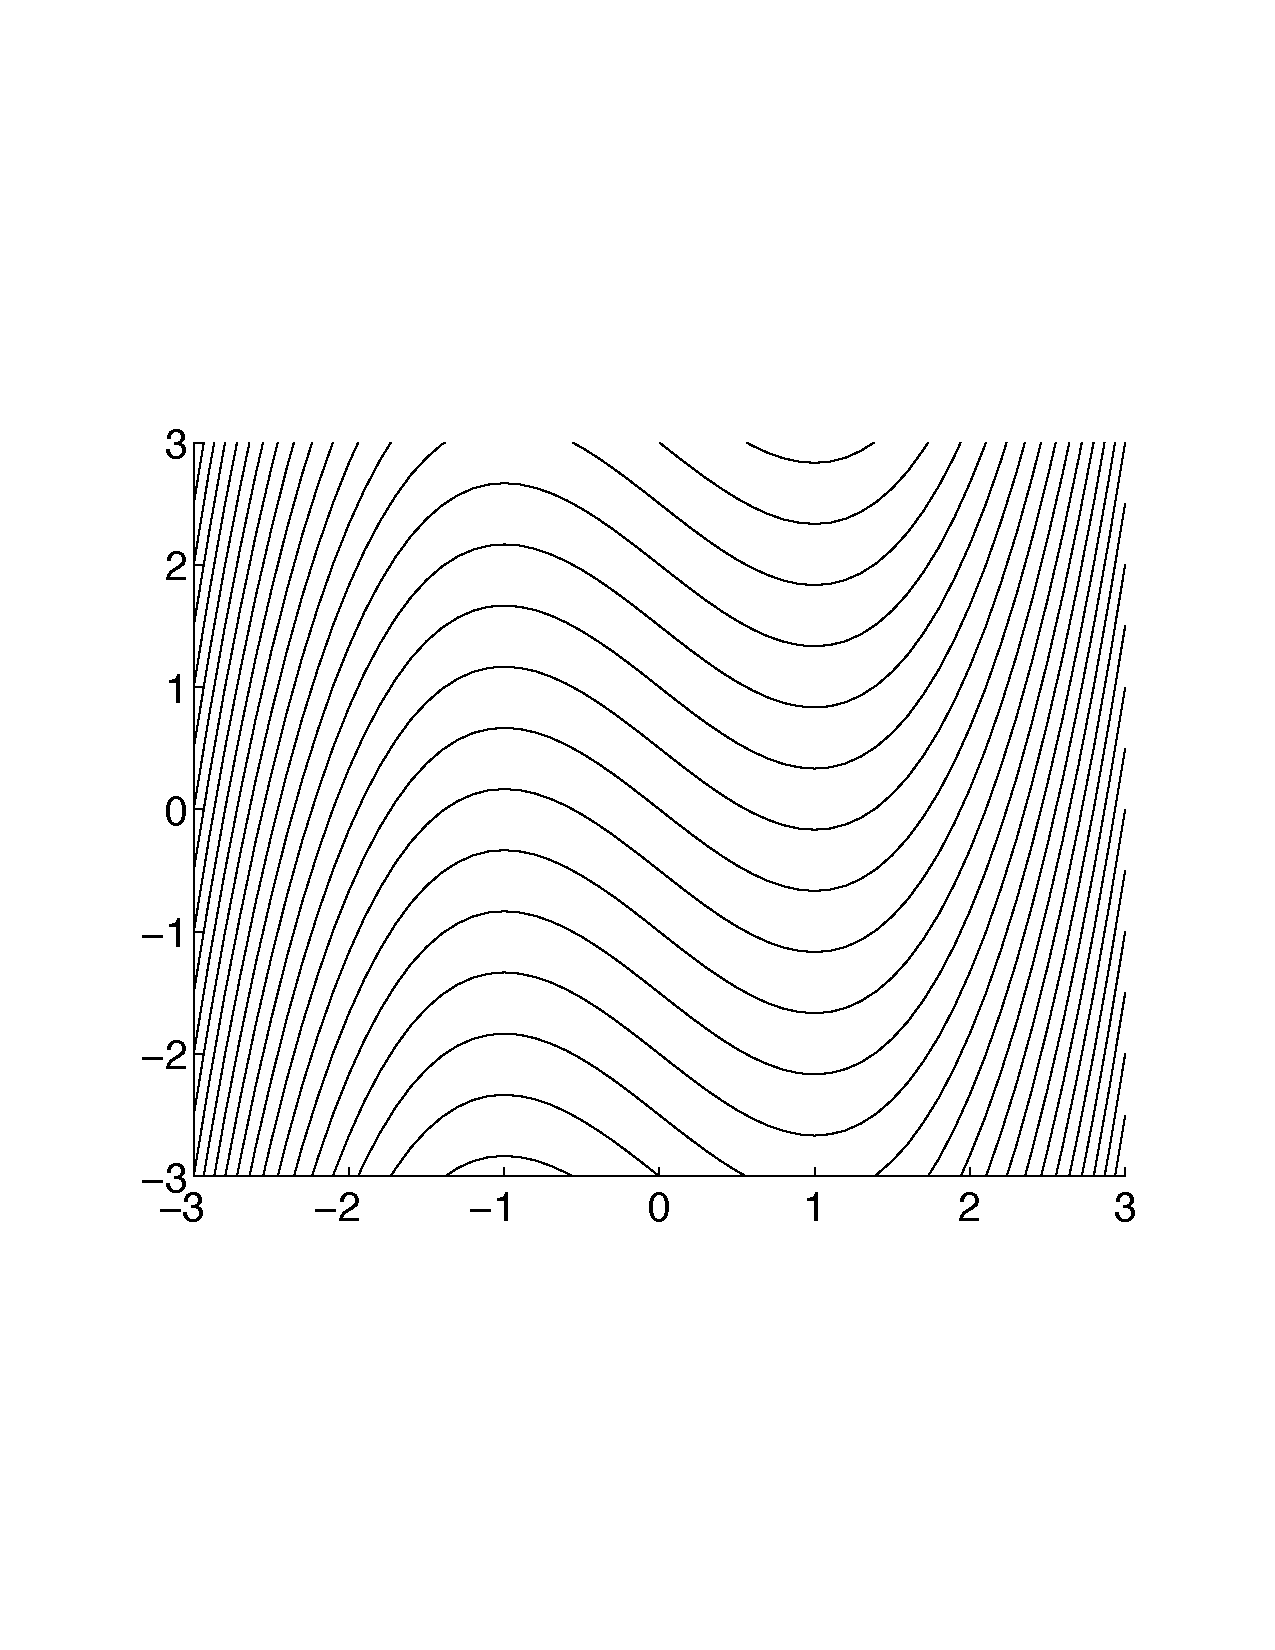
\includegraphics[width=\len, page=1]{images/module8-figs.pdf}
%			& 
%		%		\begin{tikzpicture}
%		%	    \begin{scope}
%		%	    \clip (-3,-3) rectangle (3,3);
%		%		\foreach \k in {-9,-8, ..., 36} {
%		%	      \draw[samples=50,domain=-3:3,variable=\x] plot ({\x},{-\k/3+(\x*\x)});
%		%	    }
%		%	    \end{scope}
%		%	    \draw[thick] (-3,-3) -- (-3,3);
%		%	    \draw[thick] (-3,-3) -- (3,-3);
%		%	    \foreach \k in {-3,-2, ..., 3} {
%		%	      \draw ({\k,-3}) node[below] {\tiny $\k$};
%		%	      \draw ({-3,\k}) node[left] {\tiny $\k$};
%		%	    }
%		%	\end{tikzpicture}
%		\includegraphics[width=\len, page=5]{images/module8-figs.pdf}
%			& \includegraphics[width=\len, page=4]{images/module8-figs.pdf} \\
%		D & E & F \\
%		\end{tabular}


\bookonlynewpage


\question

We seek a first-order ordinary differential equation 
\quad $y' = f(x)$ \quad 
whose solutions satisfy
$$
\begin{cases}
y(x)  \mbox{ is increasing if } x<2 \\
y(x) \mbox{ is decreasing if } 2 < x < 4 \\
y(x) \mbox{ is increasing if } x > 4
\end{cases}
$$
%
Write down or graph an $\pmb{f(x)}$ that would produce such solutions.




\bookonlynewpage

\question

Consider the ODE \quad $y'(t) = \big(y(t)\big)^2$ \quad .
Which of the following is true?
	
\begin{parts}
	\item $y(t)$ must always be positive
	\item $y(t)$ must always be negative \\[5pt]

	\item $y(t)$ must always be decreasing
	\item $y(t)$ must always be increasing
\end{parts}




\bookonlynewpage

\question Consider the differential equation $2xy'=y$.
	
	\begin{parts}
		\item Check that the curves of the form $y^2 + C x = 0$ satisfy the differential equation.
		\item Sketch one solution of the differential equation.
		\item Sketch all the integral curves for the differential equation.
		\item What is the difference between a solution passing through the point $(1,-1)$ and an integral curve passing through the same point?
	\end{parts}








%%%%%%%%%%%%%%%%%%%%%%%%%%%%%%%%%%%%%%%%%%%%%%%%%%%%%%%%%%%%%%%%%%%%%%%%
%		Slope Fields



%%%%%%%%%%%%%%%%%%%%%%%%%%%%%%
%
%  MODULE - Slope Fields
%
%%%%%%%%%%%%%%%%%%%%%%%%%%%%%%



\begin{module}{Slope Fields}
	%\Title{Slope Fields}
	\label{intro-slopefields}

	In this module you will learn
\begin{itemize}
	\item what is a slope field
	\item how to sketch a slope field
	\item to interpret a slope field
\end{itemize}

\hfill \\

As we saw in the previous module, once we have found a differential equation that models a situation, we often want to figure out what happens to the solution.

In this module, we will focus on getting an idea of the solutions and integral curves using what is called a \textbf{slope field}.





\begin{definition}[Slope field] Consider the equation $y' = f(x,y)$.
If we evaluate $f(x,y)$ over a rectangular grid of points, and we draw an arrow at each point $(x,y)$ of the grid with slope $f(x,y)$, then the collection of all the arrows is called a \emph{slope field}.
\end{definition}

\begin{graybox}
	
We can sketch Slope Fields with Wolfram Alpha.

For a differential equation $\dfrac{dy}{dx} = f(x,y)$, we need to input
\begin{itemize}
	\item Vector Field: $(1, f(x,y))$.
\end{itemize}

\url{http://www.wolframalpha.com/input/?i=slope+field}
\hfill \qrcode{http://www.wolframalpha.com/input/?i=slope+field}	
\end{graybox}





\begin{example}
Let us take an \hyperlink{sols-ex}{example from the previous module}.

Consider the initial-value problem
$$
\begin{cases}
	\dfrac{dy}{dx}=-\dfrac{x}{y} \\
	y(0)=-3
\end{cases}
$$

We can use this definition to sketch the slope field for the differential equation $ \dfrac{dy}{dx} = -\dfrac{x}{y}$.

We now sketch this slope field with Desmos:

\url{https://www.desmos.com/calculator/scmz6ps0or} \hfill \qrcode{https://www.desmos.com/calculator/scmz6ps0or}

Now notice that the arrows have the slope of a solution. This means that solutions will be tangent to the arrows, so we can \emph{roughly} trace the solution by following the arrows.

Below, we did just that starting with the point $(0,-3)$.

\setlength{\len}{175pt}
\begin{center}
%\begin{figure}
%\includegraphics*[width=\len]{images/module9-slopefield-ex1.png}
%\hfil
\begin{tabular}{ccc}
\includegraphics*[width=\len]{images/module9-slopefield-ex1-sol.png}
 & & 
\includegraphics*[width=\len]{images/module9-slopefield-ex1-intcurve.png}\\
approximated solution & & approximated integral curve
\end{tabular}
%\caption{Slope Field for the differential equation $\frac{dy}{dx} = -\frac{x}{y}$.
%\label{mod9-slopefield1}
%\end{figure}
\end{center}

\textbf{\textcolor{orange}{Important. }} Remember that this gives us only an approximation of the solution and integral curve. From the approximation, we can tell that the solution seems circular, but we still need to show that it is so.

\end{example}



%\setlength{\len}{150pt}
%\hspace{-1.35cm}\begin{tabular}{ccc}
%\includegraphics*[width=\len]{figures/0101_dirfield_rocket.png}
%	& \includegraphics*[width=\len]{figures/0101_intcurves_rocket.png} 
%	& \includegraphics*[width=\len]{figures/0101_rocket_pos.png} \\
%Direction field for $u$
%	& Approximations of $u$
%	& Solution $u(t)$
%\end{tabular}


%
%This particular one is:
%\href{http://www.wolframalpha.com/input/?i=direction+field+calculator&f1=%7B1%2C-9.8*x-0.75*y%2B10%7D%2Fsqrt(1%2B(-9.8*x-0.75*y%2B10)%5E2)&f=VectorPlot.vectorfunction%5Cu005f%7B1%2C-9.8*x-0.75*y%2B10%7D%2Fsqrt(1%2B(-9.8*x-0.75*y%2B10)%5E2)&f2=x&f=VectorPlot.vectorplotvariable1%5Cu005fx&f3=0&f=VectorPlot.vectorplotlowerrange1%5Cu005f0&f4=2&f=VectorPlot.vectorplotupperrange1_2&f5=y&f=VectorPlot.vectorplotvariable2%5Cu005fy&f6=0&f=VectorPlot.vectorplotlowerrange2%5Cu005f0&f7=4&f=VectorPlot.vectorplotupperrange2%5Cu005f4}{\tt Click Here}
%\hfill \qrcode{http://www.wolframalpha.com/input/?i=direction+field+calculator&f1=%7B1%2C-9.8*x-0.75*y%2B10%7D%2Fsqrt(1%2B(-9.8*x-0.75*y%2B10)%5E2)&f=VectorPlot.vectorfunction%5Cu005f%7B1%2C-9.8*x-0.75*y%2B10%7D%2Fsqrt(1%2B(-9.8*x-0.75*y%2B10)%5E2)&f2=x&f=VectorPlot.vectorplotvariable1%5Cu005fx&f3=0&f=VectorPlot.vectorplotlowerrange1%5Cu005f0&f4=2&f=VectorPlot.vectorplotupperrange1_2&f5=y&f=VectorPlot.vectorplotvariable2%5Cu005fy&f6=0&f=VectorPlot.vectorplotlowerrange2%5Cu005f0&f7=4&f=VectorPlot.vectorplotupperrange2%5Cu005f4}



\begin{video}
\begin{itemize}
	\item \qrvideo{https://youtu.be/MI2xCwBekX4}
	\item \qrvideo{https://youtu.be/8Amgakx5aII}
\end{itemize}	
\end{video}



	\begin{exercises}
		% Topics:
		% 
	\begin{problist}
	\prob Use Wolfram Alpha, Desmos, or another software to sketch the slope field for the following differential equations. Then roughly trace different solutions.
	\begin{enumerate}
		\item $y'=2y-x$
		\item $y'=xy$
		\item $y'=\cos(y)$
		\item $y'=\frac12+\cos(y)$
		\item $y'=1+\cos(y)$
		\item $y'=2+\cos(y)$
		\item $y'=\sin(xy)$
		\item $y'=\tan(x+y)$
	\end{enumerate}
	
	\prob Sketch a slope field for the following differential equation
	$$ y'=f(x,y)$$
	where 
	$$
	f(x,y) = \begin{cases}
 		-x & \text{ if } x< 1 \\
 		y & \text{ if } x \geq 1		
	\end{cases}
	$$

	\prob Sketch a slope field for the following differential equation
	$$ y'=f(x,y)$$
	where the function $f(x,y)$ satisfies all of the following properties:
	\begin{enumerate}
		\item $f(x,y)$ is continuous
		\item $f(x,y) > 0$ when $x>1$ and $y>1$
		\item $f(x,y) < 0$ when $x<-1$ and $y<-1$
		\item $f(x,y)$ depends only on $x$ when $x<-1$ and $y>1$
		\item $f(x,y)$ depends only on $y$ when $x>1$ and $y<-1$
	\end{enumerate}
	
	
	\prob 
		\begin{enumerate}
			\item On the slope field from the previous problem, show that there must exist a smooth continuous curve with horizontal lines.

			\item Show that the curve divides the $(x,y)$ plane in two parts.

		\end{enumerate}
	
	


	\prob Consider a differential equation 
	$$ y'=f(x,y)$$
	where the solutions satisfy
	$$ \lim_{x\to \infty} y(x) = 1.$$

	\begin{enumerate}
		\item What property must the slope field satisfy?

		\item Sketch a possible slope field for this differential equation.
	\end{enumerate}
	
	\end{problist}
\end{exercises}

\end{module}



\begin{lesson}
	\Title{Slope Fields}

	\Heading{Objectives}
	\begin{itemize}
		\item The second step in Mathematical modelling is to construct a representation of how the team will be attempting to solve the problem.
		\item Create a mind map of the problem. This is a structured way to brainstorm possible solutions and their requirements.
	\end{itemize}
	
	\Heading{Motivation} 

\begin{annotation}
	\begin{goals}
	\Goal{Extra Reading}
	Math Modelling: Getting started and getting solutions, Bliss-Fowler-Galluzzo
	
	\hfill \qrcode{https://m3challenge.siam.org/resources/modeling-handbook}	
	\end{goals}
\end{annotation}
	\Heading{Extra Reading} \href{https://m3challenge.siam.org/resources/modeling-handbook}{Math Modelling: Getting started and getting solutions, Bliss-Fowler-Galluzzo}

\end{lesson}




\newpage

\question
\begin{minipage}{.7\textwidth}
	A catapult throws a projectile into the air and we track the height (in metres) of the projectile from the ground as a function $y(t)$, where $t$ is the time (in seconds) that elapsed since the object was launched from the catapult. \\

	Then, the slope fields for $y(t)$ and $y'(t)$ are shown below:
\end{minipage}\hfill
\begin{minipage}{100pt}
	\includegraphics*[width=100pt]{images/module9-catapult.pdf}	
\end{minipage}






\setlength{\len}{200pt}
\begin{tabular}{cc}
\includegraphics*[height=\len]{images/module9-y.png}
	& \includegraphics*[height=\len]{images/module9-yprime.png} \\
Slope field for $y(t)$
	& Slope field for $y'(t)$
\end{tabular}

\hfill {\footnotesize(These slope fields were created using WolframAlpha)} \\

\begin{parts}
	\item On the slope field, sketch a \emph{possible} solution.	
	\item Consider the graph of $y(t)$. Does it form a parabola? Justify your answer.
\end{parts}

\begin{annotation}
	\begin{Goals}
		Students should think about the initial conditions.
		What is a possible value for $y(0)$? What is a possible value for $y'(0)$?
		Then sketch a possible solution that starts at those values. \\
		
		The equilibrium in the slope field for $y'(t)$ is called \emph{terminal velocity}. Some students might be able to identify it.
	\end{Goals}
\end{annotation}





\bookonlynewpage



\question Sketch the slope field for the following differential equations. 

\begin{parts}
	\item $y'=x$

\begin{annotation}
	\begin{Goals}
		The goal is not to be very accurate, but to capture the symmetry of each of these slope fields.
	\end{Goals}
	
\end{annotation}

	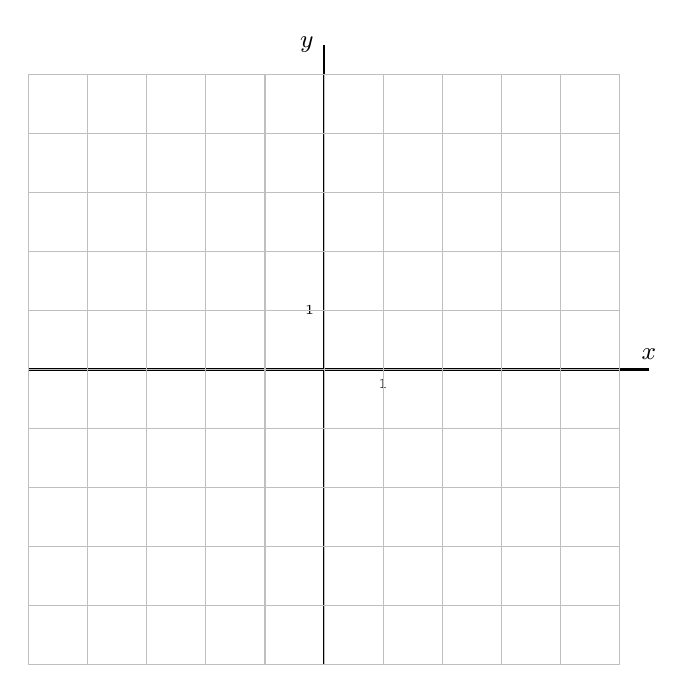
\begin{tikzpicture}[xscale=0.75,yscale=0.75]
		\draw[thick,-{\seta}] (-5,0) -- (5.5,0) node[above] {\small $x$};
		\draw[thick,-{\seta}] (0,-5) -- (0,5.5) node[left] {\small $y$};
		\draw[] (1,0) node[below] {\tiny 1};
		\draw[] (0,1) node[left] {\tiny 1};
		\draw[step=1,lightgray,thin] (-5,-5) grid (5,5);
	\end{tikzpicture}
	
	
\vfil	
	
	\item $y'=y^2$	

	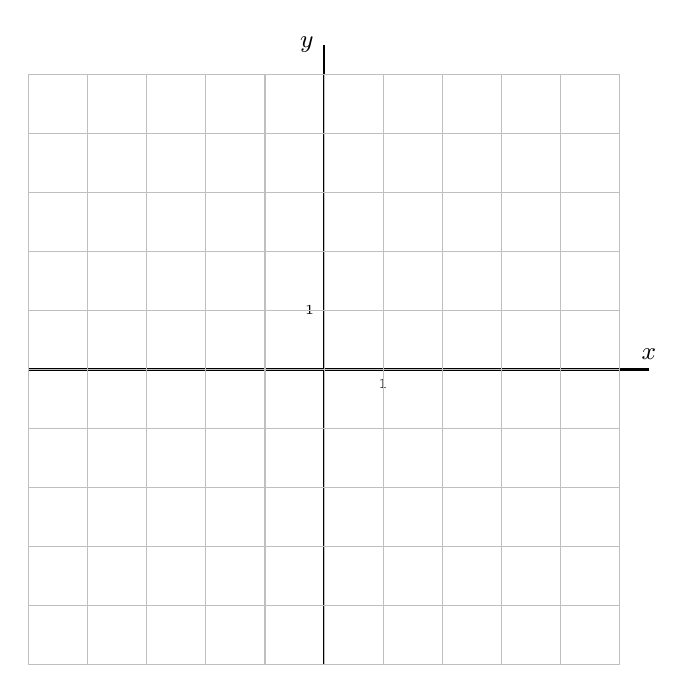
\begin{tikzpicture}[xscale=0.75,yscale=0.75]
		\draw[thick,-{\seta}] (-5,0) -- (5.5,0) node[above] {\small $x$};
		\draw[thick,-{\seta}] (0,-5) -- (0,5.5) node[left] {\small $y$};
		\draw[] (1,0) node[below] {\tiny 1};
		\draw[] (0,1) node[left] {\tiny 1};
		\draw[step=1,lightgray,thin] (-5,-5) grid (5,5);
	\end{tikzpicture}

\end{parts}



\bookonlynewpage

\question Consider the following slope fields:


\setlength{\len}{150pt}
\begin{tabular}{ccc}
	\includegraphics*[height=\len]{images/module9-graph1}
		& \includegraphics*[height=\len]{images/module9-graph2}
		& \includegraphics*[height=\len]{images/module9-graph3} \\
		(A) & (B) & (C) \\[10pt]
	\includegraphics*[height=\len]{images/module9-graph4}
		& \includegraphics*[height=\len]{images/module9-graph5}
		& \includegraphics*[height=\len]{images/module9-graph6} \\
		(D) & (E) & (F)
\end{tabular}

\hfill {\footnotesize(These slope fields were created using WolframAlpha)} \\


\begin{parts}
	\item Which slope field(s) corresponds to a differential equation of the form
		\qquad $y'=f(x)$ \qquad ?	

	\item Which slope field(s) corresponds to a differential equation of the form
		\qquad $y'=g(y)$ \qquad ?	

	\item Which slope field(s) corresponds to a differential equation of the form
		\qquad $y'=h(x+y)$ \qquad ?	

	\item Which slope field(s) corresponds to a differential equation of the form
		\qquad $y'=\kappa(x-y)$ \qquad ?	

	\item Which slope field(s) corresponds to a differential equation of the form
		\qquad $y'=1+\big( \ell(x,y) \big)^2$ \qquad ?	

	\item Which slope field(s) corresponds to a differential equation of the form
		\qquad $y'=1-\big( m(x,y) \big)^2$ \qquad ?	

\end{parts}

\begin{annotation}
	\begin{Goals}
		Students should be able to justify their choices	.
	\end{Goals}
	
\end{annotation}






\newpage




%%%%%%%%%%%%%%%%%%%%%%%%%%%%%%%%%%%%%%%%%%%%%%%%%%%%%%%%%%%%%%%%%%%%%%%%
%		Numerical Methods


\begin{module}{Numerical Methods}\label{NumericalMethods}
	%\Title{Numerical Methods}	
	\Heading{Objectives}
	\begin{itemize}
		\item Bla bla bla	
	\end{itemize}
	
	\Heading{Motivation} 


\end{module}











%%%%%%%%%%%%%%%%%%%%%%%%%%%%%%%%%%%%%%%%%%%%%%%%%%%%%%%%%%%%%%%%%%%%%%%%
%
%		Chapter 3 - First-order Models
%
%%%%%%%%%%%%%%%%%%%%%%%%%%%%%%%%%%%%%%%%%%%%%%%%%%%%%%%%%%%%%%%%%%%%%%%%




%%%%%%%%%%%%%%%%%%%%%%%%%%%%%%%%%%%%%%%%%%%%%%%%%%%%%%%%%%%%%%%%%%%%%%%%
%
%		Chapter 3 - First-Order Models
%
%%%%%%%%%%%%%%%%%%%%%%%%%%%%%%%%%%%%%%%%%%%%%%%%%%%%%%%%%%%%%%%%%%%%%%%%


\begin{topic}[First-Order Models]

\end{topic}



%%%%%%%%%%%%%%%%%%%%%%%%%%%%%%%%%%%%%%%%%%%%%%%%%%%%%%%%%%%%%%%%%%%%%%%%
%		Separable ODEs


\begin{module}{Separable ODEs}
	%\Title{Separable ODEs}
	\Heading{Textbook}	
	\Heading{Objectives}
	\begin{itemize}
		\item Bla bla bla	
	\end{itemize}
	
	\Heading{Motivation} 


\end{module}



%%%%%%%%%%%%%%%%%%%%%%%%%%%%%%%%%%%%%%%%%%%%%%%%%%%%%%%%%%%%%%%%%%%%%%%%
%		First-Order Linear ODEs


\begin{module}{First-Order Linear ODEs}
	%\Title{First-Order Linear ODEs}
	\Heading{Textbook}	
	\Heading{Objectives}
	\begin{itemize}
		\item Bla bla bla	
	\end{itemize}
	
	\Heading{Motivation} 


\end{module}












%%%%%%%%%%%%%%%%%%%%%%%%%%%%%%%%%%%%%%%%%%%%%%%%%%%%%%%%%%%%%%%%%%%%%%%%
%
%		Chapter 4 - Higher-Order Models
%
%%%%%%%%%%%%%%%%%%%%%%%%%%%%%%%%%%%%%%%%%%%%%%%%%%%%%%%%%%%%%%%%%%%%%%%%


%%%%%%%%%%%%%%%%%%%%%%%%%%%%%%%%%%%%%%%%%%%%%%%%%%%%%%%%%%%%%%%%%%%%%%%%
%
%		Chapter 4 - Higher-Order Models
%
%%%%%%%%%%%%%%%%%%%%%%%%%%%%%%%%%%%%%%%%%%%%%%%%%%%%%%%%%%%%%%%%%%%%%%%%


\begin{topic}[Higher-Order Models]



\vfil

\begin{center}
\begin{minipage}{500pt}
	\includegraphics*[width=500pt]{images/chap4-xkcd.png}

	\hfill {\footnotesize (image from \href{https://www.xkcd.com/226/}{xkcd - comic \#226})}
\end{minipage}
\end{center}


\end{topic}












%%%%%%%%%%%%%%%%%%%%%%%%%%%%%%
%
%  MODULE - Modelling with Second-Order ODEs
%
%%%%%%%%%%%%%%%%%%%%%%%%%%%%%%



\begin{module}{Modelling with Second-Order ODEs}
	\label{2nd:model}

	In this module you will learn
\begin{itemize}
	\item how to model physical phenomena to obtain second-order ODEs
\end{itemize}

\hfill \\


Whenever we model the movement of objects, we often find ourselves using \emph{Newton's Second Law of motion}:

\begin{definition}[Newton's Second Law of Motion]
	$F = m \cdot a$, \quad
	where $a$ is the acceleration of the object, $m$ is its mass, and $F$ is the net force acting on the object.
\end{definition}

Because this ``Law'' includes the acceleration of the object, and we know that
$$
{\rm acceleration} = a = \frac{d\,({\rm velocity})}{dt} = \frac{d\,v}{dt} = \frac{d^2 \, ({\rm position})}{dt^2} = \frac{d^2\,r}{dt^2},
$$
we will often end up with a Second-Order ODE.

Just like we did in module \ref{model-odes}, we will follow the step by step procedure developed in chapter 1.

\paragraph{\emph{Step 1.}} Define the problem

\begin{example}

\begin{minipage}{.75\textwidth}
We want to model the position of an object attached to the end of a spring. \\

The first step is to decide on what we want to find at the end of the process. 
So we define:
\begin{itemize}
	\item $y(t) =$ the vertical position of the mass, where $y=0$ is the position of the mass at rest.
\end{itemize}
\end{minipage}
\hfill
\begin{minipage}{44pt}
\includegraphics*[height=100pt]{images/module16-spring-mass-dashpot.pdf}	
\end{minipage}
\end{example}


\paragraph{\emph{Step 2.}} Build a mind map

\begin{example}
We start with the mass and then we brainstorm about the things that affect the mass:
\begin{center}
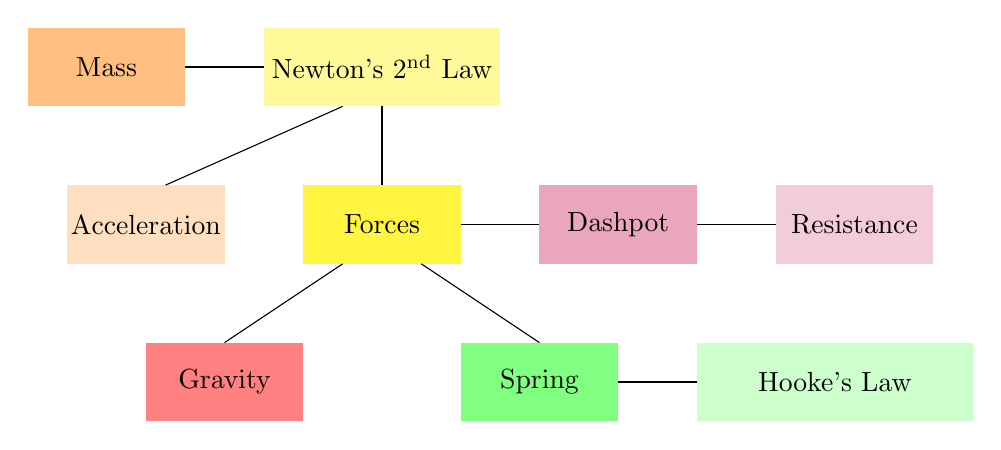
\begin{tikzpicture}
    \fill[color=orange!50!white] (-4.5,2) rectangle (-2.5,3) node[pos=.5] {\color{black}Mass};
%    \draw (-3.5,2) -- (-3.25,1);
    \fill[color=orange!25!white] (-4,1) rectangle (-2,0) node[pos=.5] {\color{black}Acceleration};
    \draw (-0.5,2) -- (-2.75,1);
    \draw (-2.5,2.5) -- (-1.5,2.5);
    \fill[color=yellow!40!white] (-1.5,2) rectangle (1.5,3) node[pos=.5] {\color{black}Newton's $2^{\rm nd}$ Law};
    \draw (0,1) -- (0,2);
  \fill[color=yellow!75!white] (-1,0) rectangle (1,1) node[pos=.5] {\color{black}Forces};
    \draw (-0.5,0) -- (-2,-1);
    \fill[color=red!50!white] (-1,-1) rectangle (-3,-2) node[pos=.5] {\color{black}Gravity};
    \draw (0.5,0) -- (2,-1);
    \fill[color=green!50!white] (3,-2) rectangle (1,-1) node[pos=.5] {\color{black}Spring};
    \draw (3,-1.5) -- (4,-1.5);
    \fill[color=green!20!white] (4,-2) rectangle (7.5,-1) node[pos=.5] {\color{black}Hooke's Law};
    \draw (1,0.5) -- (2,0.5);
    \fill[color=purple!35!white] (2,0) rectangle (4,1) node[pos=.5] {\color{black}Dashpot};  
    \draw (4,0.5) -- (5,0.5);
    \fill[color=purple!20!white] (5,0) rectangle (7,1) node[pos=.5] {\color{black}Resistance};  
\end{tikzpicture}
\end{center}
	
\end{example}


\paragraph{\emph{Step 3.}} Make assumptions

\begin{example}
In this step, we discuss the mind map we created and how we plan to address each of the boxes, or only some of the boxes. This will involve making assumptions and providing an explanation to the assumptions we make.

\begin{enumerate}
	\item As we described before the example, the plan is to use Newton's Second Law of Motion to describe the motion of the mass. This involves three quantities:
	\begin{itemize}
		\item mass: we assume that this is known to the modeller;
		\item acceleration: as we mentioned above, this is directly related to the position of the object. We have $y''(t)=$ acceleration, as long as we are assuming that the object is moving only vertically;
		\item forces: we need to find all the forces acting on the object and add them.
	\end{itemize}
\end{enumerate}

The forces acting on the object need to be discussed separately:
\begin{itemize}
	\item Gravity: we will go on a limb here and say that the force of the spring is much larger, so we will ignore this force;
	\item Spring: the force of the spring that acts on the mass follows Hooke's Law that says that the force is proportional to the extension/contraction of the spring. The constant of proportionality depends on the spring and we assume that it is known;
	\item Dashpot: the dashpot provides resistance. We will assume that it provides linear resistance to movement: the force is proportional to the velocity, with a proportionality constant that depends on the dashpot and is assumed to be known to the modeller.
\end{itemize}
	
\end{example}


\paragraph{\emph{Step 4.}} Construct a model

\begin{example}
We will start with Newton's Second Law of motion:
\begin{itemize}
	\item $m y''(t) = F(t)$ \\
\end{itemize}

and we will  add the different forces one by one:
\begin{itemize}
	\item Spring: the force of the spring is \quad $- k y(t)$; \hfill (you should check that the sign makes sense)
	\item Dashpot: the force of the dashpot is \quad $- \gamma y'(t)$. \hfill (you should also check the sign of this term) \\
\end{itemize}

Right now we have the following model:
$$
m y''(t) = -ky(t) - \gamma y'(t).
$$

\end{example}



\paragraph{\emph{Step 5.}} Model assessment

We'll skip this part here, but you should try to develop some tests to check the validity of the model we came up with.
Specifically, the fact that we ignored gravity should be checked to make sure that it doesn't affect our model too much.

\paragraph{\emph{Step 6.}} Putting it all together in a report

We'll skip this part here.





	\newpage

\begin{exercises}

	\begin{problist}
	
	\prob Consider a mountain with shape $y=f(x)$ a hiker who is climbing down the mountain with horizontal position $x(t)$. She starts at a peak of the mountain at $x_0=0$. As she climbs down the mountain, she notices that from her point-of-view, the rate of change of the slope of the mountain is decreasing linearly with time.
		The hiker also notices that her horizontal speed is constant.
	
		Model the hiker's position and the shape of the mountain.
	
	\prob 
	
	\begin{center}
		\includegraphics*[width=150pt]{images/module20-catenary.pdf}
	\end{center}

	\prob Model a ping pong ball travelling through the air.
	
	\begin{center}
		\includegraphics*[height=100pt]{images/module20-hotairballoon.pdf}
	\end{center}
	
	\prob Model an old TV floating or sinking in the ocean.
	
	\prob Model a container floating in the ocean with a leak that allows water to get inside.
	
	\prob Model a hot air balloon flying through the air.
	
	\prob Model the shape of a rope hanging between two poles.

	\begin{center}
		\includegraphics*[width=150pt]{images/module20-suspensionbridge.pdf}
	\end{center}

	\prob Model the shape of the cables of a suspension bridge.
	
	\prob Imagine a cylinder floating vertically partially submerged in a lake. Model the position of its top.
	
	\prob Model a ball rolling down a hill.
	
	\prob Model an electric circuit with a resistor, and inductor, and a capacitor in series.
	
	\prob Start with the Law of Conservation of Energy and assume a conservative force. Then show that you obtain Newton's Second Law of motion.
	
	\end{problist}
\end{exercises}

\end{module}



\begin{lesson}
	\Title{Modelling with Second-Order ODEs I}

\Heading{Textbook}
	\begin{itemize}
		\item Module 19
	\end{itemize}

\Heading{Objectives}
	\begin{itemize}
		\item Model physical phenomena to obtain a second-order ODE
		\item Understand how to use Newton's Second Law of Motion
		\item Follow the step-by-step procedure to create a model
	\end{itemize}
	
\Heading{Motivation} 

By this point, the students should have a good idea on how the modelling task goes.

Models about moving objects often require Newton's Second Law of Motion which end up having the form of a second-order ODE.

Engineering and Physics students will find models like this often in their studies.



\Heading{Preparation for Class}
\begin{itemize}
	\item Read textbook
	\item Read the core exercise \ref{2nd:keyboard} and solve steps 1 (define problem), 2 (create a mind map), and 3 (make assumptions)
\end{itemize}




\Heading{Tutorials and Projects}
\begin{itemize}
	\item Project \ref{proj:pursuit}: \pursuittitle
	\item Project \ref{proj:spring}: \springtitle
\end{itemize}




\end{lesson}




\question \label{2nd:keyboard}
	Here are some facts about laptop keys:

\begin{itemize}
\begin{minipage}{.4\textwidth}
\item[\color{Gray}(da)] Each key must also include some damping, so that it doesn't keep oscillating back and forth once pressed.

\item[\color{Gray}(di)] A typical letter key is 15mm$\times$15mm and when pressed has a maximum displacement of 0.5mm.

\item[\color{Gray}(fo)] On average, a person exerts the force of $42\,$N with one finger on a key.
\end{minipage}
\hfill
\begin{minipage}{.4\textwidth}
\item[\color{Gray}(gr)] Gravity is much weaker than the spring that keeps the key in place.

\item[\color{Gray}(hl)] Each key has a spring to make the key return to its original position after being pressed (Hooke's Law: ``the force is proportional to the extension'').

\item[\color{Gray}(lo)] Keys last 50 million presses on average.

\item[\color{Gray}(ve)] Keys can only move vertically.
\end{minipage}
\end{itemize}
	
\begin{annotation}
	\begin{goals}
		.1 should be very quick, since a very (very) similar example was solved in the module.
	\end{goals}
\end{annotation}
\begin{parts}
	\item Model a laptop keypress.
	\item What happens if the damping system of the key is broken? What happens if the damping system is too strong? How strong should the damping system be?
	\item What happens to the key when the spring breaks?
\end{parts}





\bookonlynewpage

\begin{lesson}
	\Title{Modelling with Second-Order ODEs II}

\Heading{Textbook}
	\begin{itemize}
		\item Module 19
	\end{itemize}
	
\Heading{Objectives}
	\begin{itemize}
		\item Model physical phenomena to obtain a second-order ODE
		\item Understand how to use Newton's Second Law of Motion
		\item Follow the step-by-step procedure to create a model
	\end{itemize}
	
\Heading{Motivation} 

This class, students work on a model that involves a bit more of Linear Algebra (projections) and some ``uglier'' expressions.


\Heading{Preparation for Class}
\begin{itemize}
	\item Read textbook
	\item Read the core exercise \ref{2nd:ballrolling} and solve steps 1 (define problem), 2 (create a mind map), and 3 (make assumptions)
\end{itemize}

\Heading{Tutorials and Projects}
\begin{itemize}
	\item Project \ref{proj:pursuit}: \pursuittitle
	\item Project \ref{proj:spring}: \springtitle
\end{itemize}


\end{lesson}


\begin{annotation}
	\begin{goals}
		\Goal{Ball rolling}
		Different approach depending on students. \\
		
		\emph{Students need some challenge and have time}:
		\begin{itemize}
			\item Ramp $y=f(x)$ makes it simpler
			\item Need projection (Linear Algebra) to find gravity force along the ramp at $(x_0,y_0) = \big(x_0,f(x_0)\big)$:
			$$			
			\ell = (0,-mg) \cdot (1, k)\frac{1}{\sqrt{1+k^2}} = -\frac{mgk}{\sqrt{1+k^2}}
			$$
			where $k = f'(x_0)$.
			So gravity force along the ramp is:
			$$
			\vec{F}_g = \ell (1, k)\frac{1}{\sqrt{1+k^2}} = -\frac{mgk}{1+k^2} (1,k)
			$$
			\item Yields second-order ODE 
		\end{itemize}
		\hfil
		
		\emph{Weaker students with less time}:
		\begin{itemize}
			\item Give the formula for gravity force along the ramp:
			$$
			\vec{F}_g = \ell (1, k)\frac{1}{\sqrt{1+k^2}} = -\frac{mgk}{1+k^2} (1,k)
			$$
		\end{itemize}
		
		\hfil
		
		\emph{Follow-up question}:
		\begin{itemize}
			\item Ramp is $y=(x-1)^2$
			\item Get second-order ODE for ball position
			\item Will the ball always move to the right? Justify with the ODE.
			\item Approximate near the bottom of the ramp: $y' \approx 0 \Leftrightarrow \sqrt{1+(y')^2} \approx 1$ and solve the simpler ODE.
			\item When is this approximation valid? (when ball oscillates back and forth near the bottom)
		\end{itemize}
	\end{goals}
\end{annotation}
\question \label{2nd:ballrolling}
	Model a ball rolling down a ramp.

	



\standardonlynewpage

%%%%%%%%%%%%%%%%%%%%%%%%%%%%%%
%
%  MODULE - Second-Order Linear ODEs with Constant Coefficients
%
%%%%%%%%%%%%%%%%%%%%%%%%%%%%%%



\begin{module}{Second-Order Linear ODEs with Constant Coefficients}
	\label{2nd:solving}

	In this module you will learn
\begin{itemize}
	\item how to solve this type of ODEs
\end{itemize}

\hfill \\

In this module we will learn how to solve a specific type of Second-Order ODEs: linear second-order ODEs with constant coefficients. These equations have the form
$$
a y''(t)  + b y'(t) + c y(t) = f(t).
$$

\subsection{Homogeneous ODEs}

These are ODEs above with $f(t) \equiv 0$.
So we are trying to solve
$$
a y''(t)  + b y'(t) + c y(t) = 0.
$$

The main idea to solve these problems is the same as for systems: making an \emph{educated guess} that the solution should look like an exponential:
$$
y(t) = e^{rt},
$$
and we need to find which values of $r$ yield solutions.

We do that by plugging this formula for $y(t)$ into the ODE:
\begin{itemize}
	\item $y'(t) = r e^{rt}$
	\item $y''(t) = r^2 e^{rt}$
\end{itemize}

We get
$$
a r^2 e^{rt} + br e^{rt} + c e^{rt} = 0
\quad \Leftrightarrow \quad 
	a r^2 + br + c = 0.
$$

This equation for $r$ is called the \emph{characteristic equation}.

We know how to solve it:
$$
r = \frac{-b \pm \sqrt{b^2-4ac}}{2a}.
$$

That means that we have three possible cases.





\paragraph{\color{cyan}Two real distinct roots.} When $b^2-4ac > 0$, we have two possible values for $r$ that are real numbers: $r_1$ and $r_2$.

Then, similarly to what we did with systems of ODEs, we obtain two solutions
$$
y_1(t) = e^{r_1 t} \quad \text{ and } \quad y_2(t) = e^{r_2 t},
$$
and the general solution is
$$
y(t) = c_1 e^{r_1 t} + c_2 e^{r_2 t}.
$$

\begin{video}
\begin{itemize}
	\item \qrvideo{https://youtu.be/_8fcT95JV34}
	\item \qrvideo{https://youtu.be/nE_OnX8ulHA}
	\item \qrvideo{https://youtu.be/v1xKZOrGsVc}
\end{itemize}	
\end{video}



\paragraph{\color{cyan}Two complex roots.} When $b^2-4ac<0$, we have two possible values for $r$, but they are complex values:
$$
r_{\pm} = \alpha \pm i\beta.
$$
\begin{graybox}
What are the value of $\alpha$ and $\beta$?	
\end{graybox}

Then we have two solutions
$$
y_{+}(t) = e^{(\alpha+i\beta) t} \quad \text{ and } \quad y_{-}(t) = e^{(\alpha-i\beta) t},
$$
and the general solution is
$$
y(t) = a_1 e^{(\alpha+i\beta) t}  + a_2 e^{(\alpha-i\beta) t}.
$$

Just like we did with systems with complex eigenvalues, we prefer to write the solutions without complex numbers, so we expand it using Euler's formula to get
\begin{align*}
y(t) 	& = a_1 e^{(\alpha+i\beta) t}  + a_2 e^{(\alpha-i\beta) t} \\
		& = a_1 e^{\alpha t}e^{i\beta t}  + a_2 e^{\alpha t}e^{-i\beta t} \\
		& = a_1 e^{\alpha t} \big( \cos(\beta t) + i \sin(\beta t) \big)  + a_2 e^{\alpha t} \big( \cos(\beta t) - i \sin(\beta t) \big) \\
		& = (a_1+a_2)  \cos(\beta t)e^{\alpha t} + i (a_1-a_2)\sin(\beta t) e^{a\alpha t} \\
		& = c_1 \cos(\beta t)e^{\alpha t} + c_2\sin(\beta t) e^{\alpha t}
\end{align*}

\begin{graybox}
How do $c_1$ and $c_2$ depend on $a_1,a_2$?	
\end{graybox}

So another way to write the general solution is
$$
y(t) = c_1 \cos(\beta t)e^{\alpha t} + c_2\sin(\beta t) e^{\alpha t}.
$$


\begin{video}
\begin{itemize}
	\item \qrvideo{https://youtu.be/DORl6GMPtjM?t=396}
\end{itemize}	
\end{video}




\paragraph{\color{cyan}One real repeated root.} When $b^2-4ac=0$, then we are left with only one value for $r=-\frac{b}{2a}$.

We then have one solution
$$
y_1(t) = e^{-\frac{b}{2a}t}.
$$

\begin{example}
Consider the ODE 
$$
y''(t) + 2y'(t) + y(t) = 0.
$$	

To find the general solution, we assume that the solutions have the form $y(t) = e^{rt}$, which means that $r$ must satisfy
$$
r^2 +2r+1 = 0 
	\quad \Leftrightarrow \quad r=-1,
$$
so $y_1(t) = c_1 e^{-t}$.

Now can we solve this ODE with the following initial conditions?
\begin{itemize}
	\item $y(0)=2$ and $y'(0)=-2$.
	\item $y(0)=2$ and $y'(0)=1$.
\end{itemize}
\end{example}

This previous example, should give a good idea on why having one value for $r$ means that we are missing something. 
We need to find a second solution $y_2(t)$. \\


\begin{graybox}
If we want to find all the divisors of $42$, and we already know that $d_1=2$ is a divisor, then we can use the divisor $d_1$ we know to write 
$$
d_1 \cdot x = 42 
	\quad \Leftrightarrow\quad 2x = 42
	\quad \Leftrightarrow\quad x = 21,
$$
where $x$ is the product of all the other divisors.

We used the divisor we knew $d_1$ to obtain a simpler problem for the other divisors.
\end{graybox}


\subparagraph{\color{cyan}Reduction of Order.} The idea here is the same. We use the solution we found to try to obtain a simpler ODE for the other solution:
$$
y(t) = y_1(t) \cdot u(t),
$$
where $y(t)$ is the solution we are still missing, $y_1(t)$ is the solution we already found, and $u(t)$ is a function. If we find $u(t)$, then we find $y(t)$. We hope that the function $u(t)$ satisfies a simpler problem.

To do that, we need to plug the formula above for $y(t)$ into the original ODE. 

\begin{important}
You should do these calculations yourself.
Remember to use the product rule and to be careful not to make any mistakes.	

Also remember that we know the value of $r$.
\end{important}

We obtain
$$
u''(t) = 0
\quad \Leftrightarrow \quad u(t) = c_1 + c_2 t.
$$

This means that we found 
$$
y(t) = (c_1 + c_2 t) e^{rt}
\quad \Leftrightarrow \quad y(t) = \underbrace{c_1 e^{rt}}_{\substack{\rm previous \\ \text{solution } y_1(t)}} + c_2 t e^{rt}.
$$

The general solution is 
$$
y(t) = c_1 e^{rt} + c_2 t e^{rt},
$$
where $r = -\frac{b}{2a}$.


\begin{video}
\begin{itemize}
	\item \qrvideo{https://youtu.be/DORl6GMPtjM}
\end{itemize}	
\end{video}






\subsection{Non-Homogeneous ODEs}

We are trying to solve
\begin{equation}\tag{$\star$}\label{mod20:orig}
a y''(t)  + b y'(t) + c y(t) = f(t),
\end{equation}
where $f(t)$ is a known function. \\


\begin{important}
If $u(t)$ is the general solution of
\begin{equation}\tag{$H$}\label{mod20:hom}
ay''(t)+by'(t)+cy(t) = 0,
\end{equation}
and $v(t)$ satisfies
\begin{equation}\tag{\ref{mod20:orig}}
ay''(t)+by'(t)+cy(t) = f(t),
\end{equation}
then $y(t) = u(t) + v(t)$ gives the general solution of
$$
ay''(t)+by'(t)+cy(t) = f(t).
$$

This is a practice problem at the end of this module.
\end{important}


This means that to solve this ODE, we split the general solution into two parts
$$
y(t) = y_c(t) + y_p(t),
$$
where
\begin{itemize}
	\item $y_c(t)$ is called the \emph{complementary solution} and it is the general solution of the corresponding homogenous ODE \eqref{mod20:hom}. It is solved using the technique we studied above.
	\item $y_p(t)$ is called the \emph{particular solution} and it is one function that satisfies the original ODE \eqref{mod20:orig}.
\end{itemize}

\begin{important}
It may seem strange that to solve the original ODE, we need its solution, but what we are trying to do is find \emph{all possible solutions} of the original ODE.

To find all possible solutions of the original ODE, we require two things:
\begin{itemize}
	\item \emph{One} solution of the original ODE:  $y_p(t)$,
	\item and all possible solutions of the homogeneous ODE: $y_c(t)$.
\end{itemize}
\end{important}


We already know how to find the complementary solution, so we will focus our attention on finding one particular solution.

\paragraph{\color{cyan}Method of Undetermined Coefficients.} As you probably have gotten used to by now, this is a method of educated guess-and-check. \\

Let us look at the equation from a different point-of-view
\begin{align*}
a y''(t) + by'(t) + cy(t) & = f(t) \\
\substack{\displaystyle\text{linear combination of}\\\displaystyle\text{function and derivatives}} & = f(t)
\end{align*}
and remember that some functions don't change much when differentiated:
\begin{itemize}
	\item Exponentials $y=ce^{rt}$ don't change their form after differentiation $y'=cre^{rt} = de^{rt}$. They even keep the same exponential term.
	\item Polynomials don't change their form either: their derivative is also a polynomial, with lower degree.
	\item Cosines and Sines alternate between one and the other, so functions of the form $y=c_1 \sin(rt) + c_2\cos(rt)$ don't change after differentiation.
\end{itemize}


\begin{important}
This means that, if $f(t)$ is one of these types of function, then $y(t)$ must be of the same form.	
\end{important}

\begin{example}
Find a particular solution for the ODE
$$
y''  - 4y = 10 e^{3t} = (\text{constant}) \cdot (\text{exponential of } 3t).
$$	

Our candidate is
$$
y_p(t) = A e^{3t}.
$$

Now we need to find the constant $A$ by plugging it into the ODE:
$$
9 A e^{3t} - 4 \cdot A e^{3t} = 10 e^{3t}
\quad \Leftrightarrow \quad 
	A = 2,
$$
so $y_p(t) = 2 e^{3t}$ is a particular solution.
\end{example}


\begin{example}
Find a particular solution for the ODE
$$
y''  - 4y = 3t^2+2t = (\text{polynomial of degree 2}).
$$	

Our candidate is
$$
y_p(t) = At^2 + Bt + C.
$$

Now we need to find the constants $A, B, C$ by plugging the formula for $y_p$ into the ODE:
$$
2A - 4At^2 - 4B t - 4C = 3t^2+2t
\quad \Leftrightarrow \quad 
\begin{cases}
A = -\frac34 \\
B = -\frac12 \\
C = \frac{A}{2} = -\frac38.	
\end{cases}
$$
so $y_p(t) = -\frac34 t^2 - \frac{t}{2} - \frac38$ is a particular solution.
\end{example}

There are some more details to deal with when using this method that will be addressed in the core exercises.




\begin{video}
\begin{itemize}
	\item \qrvideo{https://youtu.be/CjZ0TfPnWVU}
	\item \qrvideo{https://youtu.be/ubdSxJ2nmVk}
	\item \qrvideo{https://youtu.be/YRvqem1n0nQ}
\end{itemize}	
\end{video}





	\begin{exercises}

	\begin{problist}

	\prob Find the complementary and particular solutions for the following ODEs
	\begin{enumerate}
		\item $y''-2y'-3y=3e^{2t}$
		\item $y''-2y'-3y=-3te^{-t}$
		\item $y''-9y=t^2e^{-3t}-6$
		\item $y''+2y'-8y=e^{-t}-2e^t$
		\item $y''-y'-6y=\sin(t)$
		\item $y''-y'-6y=\sin(t)+3e^{3t}$
		\item $y''+4y=(2t+1)\sin(t) + 4\cos(2t)$
		\item $y''+y=\cos(2t)+t^3$
		\item $y''-y'-2y=t\cos(t) - t\sin(t)$
		\item $y''+5y'+6y = 2e^{-2t}$
	\end{enumerate}



	\prob What is the form of the particular solution for the ODE
	\begin{multline*}
		y^{(6)} + y^{(5)} -5 y^{(4)} + 31 y'''-176y''+220y' \\
			= (3t-1)e^{2t} + t^3e^{-5t}\sin(3t) + (4t^2-2t) e^{-2t} \sin(3t),
	\end{multline*}
	knowing that 
	\begin{multline*}
		x^6 + x^5 - 5 x^4 + 31 x^3 - 176 x^2 + 220 x \\
			= \big((x^2+2)+9\big)*(x-2)^2*x*(x+5)\quad ?
	\end{multline*}

	\prob What is the form of the particular solution for the ODE
	\begin{multline*}
		y'''' - 4 y''' + 10y'' - 12 y' + 5y \\
			= t e^t + t^2 \cos(2t) - (2t+1) e^t \sin(t),
	\end{multline*}
	knowing that 
	\begin{multline*}
		x^4 - 4x^3 + 10 x^2 - 12 x + 5 \\
			= (x-1)^2 \big( (x-1)^2+4\big)\quad  ?
	\end{multline*}

	\prob Consider the ODE
	$$
	t^2 y''+ty'-9y = 0,
	$$
	and a solution $y_1(t) = t^3$.
	
	\begin{enumerate}
		\item Use the reduction of order technique to deduce the general solution to this problem.
		
		{\bf Hint.} You should find a second-order ODE for $u(t)$ without the term $u(t)$. So define $v(t) = u'(t)$ and solve the first-order ODE for $v(t)$.
		
		
			%	Solution: $tu'' + 7 u' = 0$ \\
			%	Define: $v = u'$ \\
			%	Solve: $tv' + 7 v = 0 \Rightarrow v = c_2 t^{-7}$ \\
			%	Then: $u = \int v = c_2 \int e^{t^2} dt + c_1$


		
		
		\item Find the solution with initial conditions $y(1)=1$ and $y'(1)=-3$.
		\item Find the solution with initial conditions $y(1)=1$ and $y'(1)=3$.
		\item Find the solution with initial conditions $y(1)=1$ and $y'(1)=0$.
	\end{enumerate}


	\prob Consider the ODE
	$$
	t^2 y'' - 3 t y' + 4 y = 0
	$$
	and a solution $y_1(t) = t^2$.
	
	\begin{enumerate}
		\item Use the reduction of order technique to deduce the general solution to this problem.
		
	
			%	Solution: $tu'' + 7 u' = 0$ \\
			%	Define: $v = u'$ \\
			%	Solve: $tv' + 7 v = 0 \Rightarrow v = c_2 t^{-7}$ \\
			%	Then: $u = \int v = c_2 \int e^{t^2} dt + c_1$
		
		\item Find the solution with initial conditions $y(1)=1$ and $y'(1)=2$.
		\item Find the solution with initial conditions $y(1)=0$ and $y'(1)=1$.
	\end{enumerate}



	
	\prob Consider the ODE $a y'' +by'+cy = f(t)$, with complementary solution $y_c(t) =c_1 y_1(t) + c_2 y_2(t)$ and particular solution $y_p(t)$.
	
	Consider also the initial conditions $y(0)=y_0$ and $y'(0)=v_0$.
	
	Show that there exist constants $c_1, c_2$ such that $y(t) = y_c(t) + y_p(t)$ solves the ODE with these initial conditions.
	
	\end{problist}
\end{exercises}

\end{module}



\begin{lesson}
	\Title{Second-Order Linear ODEs with Constant Coefficients I}

\Heading{Textbook}
	\begin{itemize}
		\item Module 20
	\end{itemize}

\Heading{Objectives}
	\begin{itemize}
		\item Understand the main idea: assuming the solution is $y=e^{rt}$ and find $r$
		\item Know how to find the characteristic equation and its solutions
		\item Find the general solution of a homogeneous ODE
	\end{itemize}
	
\Heading{Motivation} 


In this section we learn how to solve second-order linear ODEs with constant coefficients.

We do that by assuming that the solution is an exponential of the form $y=e^{rt}$. The intuition behind this comes from the systems of ODEs that we just studied.

Just like with systems, there are three possible cases, but its much simpler to solve them (especially the complex case).

In this lesson, solve the core exercises \ref{2nd:ode1}--\ref{2nd:ode3} for the complementary solutions.

\Heading{Preparation for Class}
\begin{itemize}
	\item Read textbook: Homogeneous ODEs
	\item Watch corresponding video
	\item Solve the core exercise \ref{2nd:ode1}.1
\end{itemize}


\Heading{Tutorials and Projects}
\begin{itemize}
	\item Project \ref{proj:spring}: \springtitle
\end{itemize}

\end{lesson}




\question \label{2nd:ode1}
	Consider the ODE \quad $y''(t) -9y(t) = f(t)$.
\begin{parts}
	\item Find a complementary solution.
	\item Find a particular solution for $f(t) = 14 e^{-4t}$.
	\item Find a particular solution for $f(t) = 9 e^{-3t}$.
	\item Find a particular solution for $f(t) = 10\cos(t)$.
\end{parts}

\bookonlynewpage

\question \label{2nd:ode2}
	Consider the ODE \quad $y''(t) -2y'(t)+5y(t) = f(t)$. %(roots $r = 1 \pm 2i$)
\begin{parts}
	\item Find a complementary solution.
	\item Find a particular solution for $f(t) = \sin(2t)e^t$.
	\item Find a particular solution for $f(t) = (4t+2)\sin(2t)e^t$.
\end{parts}




\bookonlynewpage


\question \label{2nd:ode3}
	Consider the ODE \quad $y'' + 3y' = 3t$.
\begin{parts}
	\item Find the complementary solution.
	\item Find a particular solution.
	\item Find the solution that also satisfies
	$$ \begin{cases}
		y(0)=0 \\
		y'(0)=0
	\end{cases}$$
\end{parts}


\begin{lesson}
	\Title{Second-Order Linear ODEs with Constant Coefficients II}

\Heading{Textbook}
	\begin{itemize}
		\item Module 20
	\end{itemize}

\Heading{Objectives}
	\begin{itemize}
		\item Write the solution of a non-homogeneous ODE as $y=y_c+y_p$
		\item Use the Method of Undetermined Coefficients to find a particular solution
	\end{itemize}
	
\Heading{Motivation} 

This will include some more linear algebra! 

The Method of Undetermined Coefficients is very computational once the students have some practice with it. A good way to learn it is by giving only partial information and let students struggle a little before showing how to proceed: 
\begin{itemize}
	\item that's the idea behind core exercise \ref{2nd:ode1}, where the first two exercises are straight forwards, but then without more information the students will struggle to find the particular solution.
	\item After a little struggle in lecture, the instructor can then show the way.
\end{itemize}


In this class, solve the core exercises \ref{2nd:ode1}--\ref{2nd:ode3} for the particular solutions.

\Heading{Preparation for Class}
\begin{itemize}
	\item Read textbook: Non-Homogeneous ODEs
	\item Watch corresponding video
	\item Solve the core exercise \ref{2nd:ode2}.2-3.
\end{itemize}




\Heading{Tutorials and Projects}
\begin{itemize}
	\item Project \ref{proj:spring}: \springtitle
	\item Project \ref{proj:wing}: \wingtitle
\end{itemize}


\end{lesson}




\standardonlynewpage

%%%%%%%%%%%%%%%%%%%%%%%%%%%%%%
%
%  MODULE - Analysis of Higher Order ODEs
%
%%%%%%%%%%%%%%%%%%%%%%%%%%%%%%



\begin{module}{Analysis of Models with Higher Order ODEs}
	\label{2nd:analysis}

	In this module you will learn
\begin{itemize}
	\item different ways to analyze models with higher-order differential equations
\end{itemize}

\hfill \\



In this chapter, we have learned how to create models involving systems of ODEs and how to solve some special types of second-order ODEs.



In this module, we'll study one example using a few different methods.

\begin{example}
Consider the model we found earlier for a mass attached to a spring:

\begin{minipage}{0.85\textwidth}
\begin{itemize}
	\item $y(t)=$ vertical position of the mass, where $y=0$ is the position of the mass at rest
	\item $my''(t) = -k y(t) - \gamma y'(t)$
	\item $m,k,\gamma>0$ are constants for the mass, the stiffness of the spring, and the resistance of the dashpot.
\end{itemize}
\end{minipage}
\begin{minipage}{50pt}
\includegraphics*[height=100pt]{images/module16-spring-mass-dashpot.pdf}	
\end{minipage}
\end{example}

\hfill

\begin{center}
\textbf{\color{cyan}
Qualitative evolution of quantities
}
\end{center}


We can try to figure out how these quantities, $y(t)$, $y'(t)$, and $y''(t)$ are going to increase or decrease as time goes by. \\

Let us imagine that initially  \quad $y(0)=1, y'(0)=0$.

Then, at $t=0$, we have
$$
\begin{cases}
y(0)=1 \\
y'(0)=0 \\
y''(0)= -k < 0 & \text{ (so object is decelerating, meaning speed will become negative)}
\end{cases}
$$

This means that the object is decelerating, so we have two immediate consequences:
\begin{itemize}
	\item the speed will decrease and become negative
	\item the position will start decreasing
\end{itemize}

Once the speed is negative, we see another effect
$$
y''(t) = -k\underbrace{y(t)}_{\text{decreasing}} \underbrace{- \gamma y'(t)}_{\rm positive},
$$
so the acceleration is negative but approaching zero at time $t_1$:
$$
0=y''(t_1) = -ky(t_1) - \gamma y'(t_1)
\quad \Leftrightarrow \quad k y(t_1) = - \gamma y'(t_1)
$$

Let us summarize our results so far in a table:

\begin{graybox}
\begin{center}
\begin{tabular}{c||c|c|c|c|c|c|c|c}
$\pmb{t}$	& $0$ 		& 			& $t_1$ &  			& 			& 	&	& \hspace{1cm} $+\infty$ \\[5pt] \hline\hline
$\pmb{y}$ & $1$	& $ \searrow$	& $+$ &	$\searrow$ 	&	&  \hspace{0.5cm}	&  	& 	\\[5pt] \hline
$\pmb{y'}$ & $0$ &	$\searrow$	& $-$ & $\nearrow$ & 	&  	& &	\\[5pt] \hline
$\pmb{y''}$ & $-$		& $\nearrow$ & 0  & $\nearrow$  & 	& 	&  &	\\[5pt] \hline
\end{tabular}
\end{center}
\end{graybox}

The next milestone is:
$$
y(t_2)=0 \quad \text{ or } \quad y'(t_2)=0.
$$

If $y'(t_2)=0$ while $y(t_2)>0$, then 
$$
y''(t_2) = -ky(t_2) <0,
$$
which means that $y''$ would have had to decrease again, become zero and then negative, so there would have been another milestone before.
We deduce that the next milestone is
$$
y(t_2)=0
\quad \Leftrightarrow \quad	
	y''(t_2) = -\gamma y'(t_2) > 0.
$$

\begin{graybox}
\begin{center}
\begin{tabular}{c||c|c|c|c|c|c|c|c}
$\pmb{t}$	& $0$ 		& 			& $t_1$ &  			&	$t_2$& 	&$t_3$	& \hspace{1cm} $+\infty$ \\[5pt] \hline\hline
$\pmb{y}$ & $1$	& $ \searrow$	& $+$ &	$\searrow$ 	& $0$	&  $\searrow$ 	& $-$ 	& $\cdots$	\\[5pt] \hline
$\pmb{y'}$ & $0$ &	$\searrow$	& $-$ & $\nearrow$ & $-$	&  $\nearrow$	& $0$ &	$\cdots$ \\[5pt] \hline
$\pmb{y''}$ & $-$		& $\nearrow$ & 0  & $\nearrow$  & $+$ & $\nearrow$	& $+$ &	$ \cdots$ \\[5pt] \hline
\end{tabular}
\end{center}
\end{graybox}

We can continue this analysis to conclude that the position seems to cycle back and forth between positive and negative, like you would expect from a spring. \\

\begin{graybox}
In fact, this \emph{study is flawed}, since there is a possibility that the time $t_1$ never happens and the spring only approaches the state described without ever reaching it. This will happen for some configuration of the constants $m,k,\gamma$.
\end{graybox}




\hfill

\begin{center}
\textbf{\color{cyan}
Properties of the solutions
}
\end{center}



We learned earlier in the chapter how to solve this type of differential equations.

To solve them, we assume that solutions are of the form $y=e^{rt}$ and then find a characteristic equation for $r$:
$$
mr^2 = -k - \gamma r
\quad \Leftrightarrow \quad 
r = \frac{-\gamma \pm \sqrt{\gamma^2 - 4mk}}{2m}.
$$

Depending on the constants $m, k, \gamma$, we can have:
\begin{itemize}
	\item Two real distinct solutions 
	\item Two complex distinct solutions
	\item One repeated real solution
\end{itemize}

How do solutions behave in each case?
What kind of springs or dashpots imply each case?





\hfill

\begin{center}
\textbf{\color{cyan}
Limiting behaviour of the solutions
}
\end{center}


From the analysis done above, we see that the possible values for $r$ are either negative or when $r$ is complex, its real part is negative (why?).

This means that the solution will have the form
$$
y(t) = e^{(\text{negative constant}) t} \left[  a\cos(\alpha t) + b\sin(\beta t) + c\right],
$$
so 
$$
\lim_{t \to \infty} y(t) = 0.
$$

This means that the mass will slow down and eventually stop.


%\newpage
\hfill

\begin{center}
\textbf{\color{cyan}
Numerical approximations
}
\end{center}



In module \ref{ODE:approximation} we learned how to approximate solutions of first-order ODEs using Euler's Method.

We can extend that method to second-order ODEs, which we will leave as an exercise, and approximate the solution:

\begin{center}
\begin{tabular}{ccc}
\includegraphics*[width=125pt]{images/module21-approx-k2g5.png}
	& \includegraphics*[width=125pt]{images/module21-approx-k2g1.png}
	& \includegraphics*[width=125pt]{images/module21-approx-k2g0.png} \\
$k=2,\gamma=5$ 
	& $k=2,\gamma=1$ 
	& $k=2,\gamma=0$
\end{tabular}
\end{center}

These graphs also give us some intuition on how the solutions behave.

\begin{graybox}
You can access this simulation here:
\begin{itemize}
	\item \qrvideo{https://www.desmos.com/calculator/mufgdgku9w}
\end{itemize}	
\end{graybox}















	%\newpage 

\begin{exercises}

	\begin{center}
		\includegraphics*[height=100pt]{images/module20-hotairballoon.pdf}
	\end{center}

	\begin{problist}
	
	\prob Consider the model for a hot air balloon:
	\begin{itemize}
		\item $y(t) = $ altitude of the balloon;
		\item $y''(t) = \underbrace{-g}_{\rm gravity} + \underbrace{\big( g - 9 (y-1000) \big)}_{\rm lift} + p(t)$;
		\item $g=$ gravitational constant;
		\item $p(t)=$ passenger actions affecting the vertical acceleration of the balloon.
	\end{itemize}
	\begin{enumerate}
		\item What is the equilibrium altitude?
		\item How does the balloon behave without passenger actions?
		\item If the passenger actions are $p(t) = 6 \cos(\omega t)$, study how the constant $\omega$ changes the behaviour.
	\end{enumerate}
	

	

	\prob Consider the model for a cubic object floating/sinking in the ocean:
	\begin{itemize}
		\item $d(t) = $ depth of the object;
		\item $m d''(t)  = -mg - \gamma \big|d'(t)\big| d'(t) + A r^3$;
		\item $m=$ mass of the object;
		\item $r=$ length of one side of the object;
		\item $\gamma=$ water resistance constant;
		\item $A=$ buoyancy constant (density of water minus density of object).
	\end{itemize}

	\begin{enumerate}
		\item Does the object float or sink? 
		\item What is the terminal vertical velocity of the object?
		\item Assume the constants $r=\frac12$m, $m=30$kg, $\gamma =1$kg/m, $A=300 \cdot 2^3$kg/(ms)$^2$, and approximate $g\approx 10$m/s$^2$. Assume that the initial depth of the object is 0m (the surface of the ocean). 
			
			What is the object's terminal velocity?
			Will it reach the bottom of the ocean?
	\end{enumerate}
	
	
	\begin{center}
		\includegraphics*[width=50pt]{images/module22-spring-mass.pdf}
	\end{center}

	
	\prob Consider the following model for a spring-mass system:
	\begin{itemize}
		\item $y(t) = $ position of the mass;
		\item $y''(t)  = -ky(t) + f(t)$;
		\item $k=$ stiffness of the spring;
		\item $f(t)=$ extra force on the mass.
	\end{itemize}

	\begin{enumerate}
		\item How does the spring behave when there is no external force?
		\item Assume $k=9$. How does the spring behave when the external force is $f(t)=\cos(4t)$?
		\item Assume $k=9$. How does the spring behave when the external force is $f(t)=\cos(3t)$?
		\item Assume $k=9$. How does the spring behave when the external force is $f(t)=\cos(2.95t)$?
	\end{enumerate}
	
	
	\hspace{-1cm}\includegraphics*[width=250pt]{images/chap4-xkcd.png}
	

	
	\prob Explain how the initial statement of the comic makes sense.
		
	\end{problist}
\end{exercises}
\end{module}



\begin{lesson}
	\Title{Analysis of Models with Higher Order ODEs I}

\Heading{Textbook}
	\begin{itemize}
		\item Module 21
	\end{itemize}

\Heading{Objectives}
	\begin{itemize}
		\item Deduce properties of solutions of second-order of ODEs using different approaches
	\end{itemize}
	
\Heading{Motivation} 

As we have seen in the previous chapters, it is important to know how to analyze ODEs.

In this first lesson about the Analysis of ODEs, we start with some more qualitative properties deduced without finding the solution.

\Heading{Preparation for Class}
\begin{itemize}
	\item Read textbook
	\item Solve the core exercise \ref{2nd:analysis:ode1}.1
\end{itemize}

\Heading{Tutorials and Projects}
\begin{itemize}
	\item Project \ref{proj:pursuit}: \pursuittitle
	\item Project \ref{proj:spring}: \springtitle
	\item Project \ref{proj:wing}: \wingtitle
\end{itemize}


\end{lesson}





\question \label{2nd:analysis:ode1}
	Consider the second-order ODE:
	$$
	y''(t) - 3y(t) = t \big( 2 + \sin(t) \big).
	$$
	
\begin{annotation}
\begin{goals}
	\Goal{Without solution}
	The goal is to solve this without finding an expression for the solution.
	
	For .2, the idea is to make sure that $y''<0$. 
\end{goals}	
\end{annotation}
	\begin{parts}
		\item Assume that $y(0)=0$ and $y'(0)=b$. Which values of $b$ guarantee that $y(t)>0$ for $t\geq 0$. 
		\item Assume that $y(0)=a<0$ and $y'(0)=b$. Give an example of $a,b$ such that $y(t)$ is increasing for $t\geq 0$. 
		\item Assume that $y(0)=0$ and $y'(0)=b$. Which values of $b$ guarantee that $y(t)<0$ for all $t>0$.
\begin{annotation}
\begin{goals}
	If there is time, start the next core exercise.
\end{goals}
\end{annotation}


%\begin{align*}
%& y''(t) = t \big( 2 + \sin(t) \big)  + 3 y(t) < 0 
%	\quad \Leftrightarrow \quad 
%		y(t) < - \frac{t}{3} \big( 2 + \sin(t) \big) \\
%& y'(0) = -1 \\
%\\
%& y(0)<0, y'(0)= -1 \\
%& y''(0) < 0 \\
%	& y' \searrow \\
%	& y \searrow \\
%\end{align*}
%
%Since $y'(t)<-1$, that means $y(t) < -t$, thus
%$$
%y''(t) = 3 y(t)+ t \underbrace{\big( 2 + \sin(t) \big)}_{\leq 3}
%	< -3t + 3t 
%	= 0 
%$$
%which means that $y'$ will continue to decrease and $y$ will also continue to decrease, so it will continue to be negative.

	\end{parts}


	

\bookonlynewpage

\begin{lesson}
	\Title{Analysis of Models with Higher Order ODEs II}

\Heading{Textbook}
	\begin{itemize}
		\item Module 21
	\end{itemize}

\Heading{Objectives}
	\begin{itemize}
		\item Deduce interesting behaviours:
		\begin{itemize}
			\item Resonance
			\item Beats
		\end{itemize}
	\end{itemize}
	
\Heading{Motivation} 

As we have seen in the previous chapters, it is important to know how to analyze ODEs.

In this case, even after we find the solutions, the way they behave is hidden in the formula. We still need some work to find out the interesting behaviours that arise.

\Heading{Preparation for Class}
\begin{itemize}
	\item Read textbook
	\item Solve the core exercise \ref{2nd:analysis:ode2}.1--2
\end{itemize}

\Heading{Tutorials and Projects}
\begin{itemize}
	\item Project \ref{proj:pursuit}: \pursuittitle
	\item Project \ref{proj:spring}: \springtitle
	\item Project \ref{proj:wing}: \wingtitle
\end{itemize}


\end{lesson}

\begin{annotation}
\begin{goals}
	\Goal{Goals:}
	\begin{itemize}
		\item Learn some different types of behaviour of for second-order ODEs
		\item Learn how to sketch trig functions combined with linear or other trig functions
	\end{itemize}
	
	\hfill
	
	\begin{enumerate}[label=.\arabic*.]
		\item Complementary solution!
		\item \emph{Adding} two trig functions: one oscillating slowly and one oscillating quickly
		\item Resonance: $t$ times trig function
		\item Beats: \emph{product} of two trig functions -- one oscillating slowly and one oscillating quickly
	\end{enumerate}
\end{goals}	
\end{annotation}
\question \label{2nd:analysis:ode2}
	Consider the second-order ODE:
	$$
	\begin{cases}
	y''(t) +4 y(t) = f(t) \\
	y(0)=y_0\\
	y'(0)=0
	\end{cases}
	$$
	
	\begin{parts}
		\item Let $f(t)=0$ and $y_0=1$. Sketch the solution.
		\item Let $f(t)= 396\cos(20t)$ and $y_0=0$. Sketch the solution.
%		$$ y(t) = \cos(2t) - \cos(20t)$$

		\item Let $f(t) = -4\sin(2t)$ and $y_0=1$. Sketch the solution.
%		$$ y(t) = \cos(2t) +t\cos(2t) $$	

		\item Let $f(t) = 0.39\cos(1.9t)$ and $y_0=2$. Sketch the solution.
		
		\textbf{Hint. } $\displaystyle \cos(at) + \cos(bt) = 2 \cos\left( \frac{a-b}{2} \right)  \cos\left(\frac{a+b}{2} t \right)$
%		$$ y(t) = \cos(2t) + \cos(1.9t) = 2 \cos(0.1 t) \cos(1.95t)$$	
	\end{parts}



\standardonlynewpage



















%%%%%%%%%%%%%%%%%%%%%%%%%%%%%%%%%%%%%%%%%%%%%%%%%%%%%%%%%%%%%%%%%%%%%%%%
%
%		Chapter 5 - Discrete Models
%
%%%%%%%%%%%%%%%%%%%%%%%%%%%%%%%%%%%%%%%%%%%%%%%%%%%%%%%%%%%%%%%%%%%%%%%%


%%%%%%%%%%%%%%%%%%%%%%%%%%%%%%%%%%%%%%%%%%%%%%%%%%%%%%%%%%%%%%%%%%%%%%%%
%
%		Chapter 5 - Discrete Models
%
%%%%%%%%%%%%%%%%%%%%%%%%%%%%%%%%%%%%%%%%%%%%%%%%%%%%%%%%%%%%%%%%%%%%%%%%


\begin{topic}[Difference Equations]


%\includegraphics*[width=300pt]{images/randomwalk.png}
%
%{\footnotesize (image from \href{https://commons.wikimedia.org/wiki/File:Random_walk_in2D_closeup.png}{Wikimedia Commons} created by Oleg Alexandrov)}
%
%\begin{center}
%	\includegraphics*[width=200pt]{images/SimpleRabbits2.png}
%	
%	{\footnotesize (image from Houman Madani)}	
%\end{center}

\vfil

\begin{center}
\begin{minipage}{300pt}
	\includegraphics*[width=300pt]{images/chap5-xkcd.png}

	\hfill {\footnotesize (image from \href{https://www.xkcd.com/947/}{xkcd - comic \#947})}
\end{minipage}
\end{center}
\end{topic}











%%%%%%%%%%%%%%%%%%%%%%%%%%%%%%
%
%  MODULE - Introduction to Difference Equations
%
%%%%%%%%%%%%%%%%%%%%%%%%%%%%%%



\begin{module}{Introduction to Difference Equations}
	\label{diff:intro}

	In this module you will learn
\begin{itemize}
	\item what is a difference equation
	\item the different types of difference equations
\end{itemize}

\hfill \\[-10pt]


\begin{definition}[Difference Equation]
	A \emph{difference equation} is an equation involving an unknown sequence and a recursive relation between different terms of that sequence.
\end{definition}

\begin{example}
\begin{enumerate}
	\item $u_{k+1} = u_k + u_{k-1}$
	\item $x_k = 2 x_{k-1}$
\end{enumerate}	
\end{example}



Among difference equations, there are lots of types, that require different approaches, so we need to classify them.

\begin{definition}[Types of Differential Equations]
	Just like with differential equations, the main way we distinguish difference equations is according to:
	\begin{itemize}
		\item \emph{order}: the order of a difference equation is the difference between the highest and the smallest terms of the sequence present in the difference equation;
		\item \emph{linear} vs \emph{nonlinear}: A difference equation \quad $F\big(k,u_k,u_{k-1},\ldots,u_{k-n} \big) = 0$ \quad is called \emph{linear} if $F$ is a linear function of $u_k, u_{k-1}, \ldots,u_{k-n}$. Linear difference equations have the form
			$$ a_0(k) u_k + a_1(k) u_{k-1} + \cdots + a_n(k) u_{k-n} = b(k). $$
			All other differential equations are called \emph{nonlinear}.
	\end{itemize}
\end{definition}

\begin{graybox}
	Roughly, to check whether a difference equation is \textbf{linear}, we need to check that:
	\begin{itemize}
		\item The unknown $u_k$ and its other terms appear with exponent 1;
		\item The unknown $u_k$ and its other terms do not multiply by each other;
		\item The unknown $u_k$ and its other terms are not the objects of other functions -- there are no occurrences of things like $\sin(u_k)$ or $e^{u_{k-4}}$, $\ln(u_{k+1})$, $\sqrt{u_{k-1}}$, etc.
	\end{itemize}
\end{graybox}

\begin{example}
\begin{enumerate}
	\item The difference equation $u_{k} = 2 u_{k-2}$ is linear and second-order,because $k-(k-2) = 2$.
	\item The difference equation $u_{k+1} =  u_{k}^2+u_{k-2}$ is nonlinear and third-order, because $(k+1)-(k-2) = 3$.
\end{enumerate}	
\end{example}



Similarly to differential equations, linear difference equations are, in general, easier to study and their theory is much more developed.



	\begin{noexercises}
\end{noexercises}
\end{module}



\begin{lesson}
	\Title{Introduction to Difference Equations}

	\Heading{Objectives}
	\begin{itemize}
		\item Bla
	\end{itemize}
	
	\Heading{Motivation} 

\end{lesson}


%\newpage
%
%\question
%	Core Exercise with several parts
%\begin{parts}
%	\item Part 1
%	\item Part 2
%\end{parts}
%
%\bookonlynewpage
%
%
%\question
%	One more core exercise
%
%
%
%











%%%%%%%%%%%%%%%%%%%%%%%%%%%%%%
%
%  MODULE - Solving Difference Equations
%
%%%%%%%%%%%%%%%%%%%%%%%%%%%%%%



\begin{module}{Solving Difference Equations}
	\label{diff:solve}

	In this module you will learn
\begin{itemize}
	\item how to solve some types of difference equations
\end{itemize}

\hfill \\


%Let us start with some easier difference equations to gain some intuition on how to solve them.


%\subsection{First-order linear difference equations with constant coefficients}
%
%Let us start with a simple example.
%
%\begin{example}


Let us start with a technique that is very simple and useful, although because it is so simple, it requires some ingenuity to pull off in some cases. \\

\submodule{Expanding to find a pattern} 

We'll start with an example.

\begin{example}
Consider the initial-value problem
$$
\begin{cases}
u_{k+1} = \frac32 u_k & \text{ for } k \geq 0 \\
u_0 = 5	
\end{cases}
$$

Then we can start calculating:
\begin{itemize}
	\item $u_1 = \frac32 u_0 = 7.5$
	\item $u_2 = \frac32 u_1 = 11.25$
	\item $u_3 = \frac32 u_2 = 16.875$
	\item $u_4 = \frac32 u_3 = 25.3125$
	\item $u_5 = \frac32 u_4 = 37.96875$
	\item $\vdots$
\end{itemize}

As you can notice, it's not particularly easy to find a pattern in these numbers. 

The problem is that we \emph{over-simplified}. The trick with this technique is to simplify without over-simplifying.

Let's calculate again:
\begin{itemize}
	\item $u_1 = \frac32 u_0 = \frac32 \cdot 5$
	\item $u_2 = \frac32 u_1 = \frac32 \cdot \frac32 \cdot 5 = \left(\frac32\right)^2 \cdot 5$
	\item $u_3 = \frac32 u_2 = \frac32 \cdot \left(\frac32\right)^2 \cdot 5 = \left(\frac32\right)^3 \cdot 5$
	\item $u_4 = \frac32 u_3 = \frac32 \cdot \left(\frac32\right)^3 \cdot 5 = \left(\frac32\right)^4 \cdot 5$
	\item $u_5 = \frac32 u_4 = \frac32 \cdot \left(\frac32\right)^4 \cdot 5 = \left(\frac32\right)^5 \cdot 5$
	\item $\vdots$
\end{itemize}

Now the pattern should be clear:
$$
u_k = \left(\frac32\right)^k \cdot 5.
$$

To show that this is indeed the solution, we need to use Mathematical Induction (see appendix \ref{app:induction}) to prove it. 
\end{example}

The main idea of this technique is to calculate the terms of the fraction one by one in terms of the initial data.

This is a technique that requires practice, as it is often difficult to judge which parts to simplify and which parts to expand to make sure the pattern emerges clearly. \\

\begin{video}
\begin{itemize}
	\item \qrvideo{https://youtu.be/0OcUAjOXmFc}
\end{itemize}	
\end{video}


\hfill


\submodule{Educated Guessing}

This is the technique we used several times in the book already. We used it with systems of differential equations and with second-order differential equations.

Observe that in the last example, the solution was an exponential, as was the case with differential equations.

\begin{example}
Consider the Fibonacci sequence:
$$
\begin{cases}
f_{k+1} = f_k + f_{k-1} \\
f_0 = 0 \\
f_1 = 1	
\end{cases}
$$

We want to find a formula for $f_k$. To do that, let us assume that the sequence is an exponential. So we can assume that
$$
f_k = r^k,
$$
for some value of $r$.

Let us now use this form of $f_k$ into the difference equation to obtain:
$$
r^{k+1} = r^k + r^{k-1},
$$
which can be simplified by dividing by $r^{k-1}$:
$$
r^2 = r + 1 \quad \Leftrightarrow \quad r^2 - r - 1 = 0.
$$

This is a quadratic equation that we can solve:
$$
r_{\pm} = \frac{1 \pm \sqrt{1 + 4}}{2} = \frac{1 \pm \sqrt{5}}{2}.
$$

So we have two values of $r$ that seem to work. 

That is similar to what we had when solving second-order ODEs (and this is a second-order difference equation).
In that case, the solution turned out to be a linear combination of the two solutions found:
$$
f_k 
	\quad = \quad  c_1 r_-^k + c_2 r_+^k
	\quad = \quad  c_1 \left(\frac{1 - \sqrt{5}}{2}\right)^k + c_2 \left(\frac{1 + \sqrt{5}}{2}\right)^k.
$$

Now we need to find $c_1$ and $c_2$ using the initial data:
\begin{align*}
0 & = c_1 + c_2
	\tag{$k=0$}	 \\
1 & = \quad  c_1 \frac{1 - \sqrt{5}}{2} + c_2 \frac{1 + \sqrt{5}}{2}
	\tag{$k=1$}
\end{align*}
This yields:
\begin{align*}
c_1 & = -\frac{1}{\sqrt{5}}\\
c_2 & = \frac{1}{\sqrt{5}}	
\end{align*}

So the formula we obtain is
$$
f_k =  \frac{1}{\sqrt{5}} \left[\left(\frac{1 + \sqrt{5}}{2}\right)^k - \left(\frac{1 - \sqrt{5}}{2}\right)^k \right].
$$
\end{example}


\begin{important}
The idea of this technique is to assume that the solution is an exponential of the form $r^k$ and find the values for $r$ that solve the particular difference equation. The general solution will be a linear combination of these solutions.
\end{important}

\begin{video}
\begin{itemize}
	\item \qrvideo{https://youtu.be/A5tBvxDM9V4}
\end{itemize}	
\end{video}



	\begin{exercises}

	\begin{problist}
	\prob Consider the initial-value problem
	$$ 	\begin{cases}
			 x_{k+1} = 3 x_k + 4 \\
			 x_0 = 1
 		\end{cases} $$
 	\begin{enumerate}
 		\item Using the expand-until-you-find-the-pattern technique, find the solution of this problem.
 		\item Observe that this problem has an equilibrium solution $x^\star$. What is $x^\star$?
 		\item Define a new sequence $y_k = x_k - x^\star$. Which initial-value problem does ti satisfy?
 		\item Find $y_k$.
 		\item Find $x_k$.
 	\end{enumerate}

	\prob Find the solution to the problem
	$$ 	\begin{cases}
			 x_{k+1} = -2x_{k} +3 \\
			 x_1 = 2
 		\end{cases} $$

	\prob When we were solving ODEs, we considered exponential solutions of the form $u_k = e^{rk}$, but above we considered $u_k = r^k$. Are these equivalent?
	
	Consider the initial-value problem
	$$ 	\begin{cases}
			 x_{k+1} = x_{k} - x_{k-1} \\
			 x_0 = 1 \\
			 x_1 = 2
 		\end{cases} $$

	\begin{enumerate}
		\item Solve the problem assuming the solution is of the form $u_k = r^k$.
		\item Solve the problem assuming the solution is of the form $u_k=e^{rk}$.
		\item What can you conclude?
	\end{enumerate}


	\prob Find the solution to the problem
	$$ 	\begin{cases}
			 x_{k+1} = -2x_{k} - x_{k-1} \\
			 x_0 = 1 \\
			 x_1 = 2
 		\end{cases} $$
	
	\prob Find the solution for the problem
	$$ 	\begin{cases}
			 a x_{k+1} - x_k + (1-a) x_{k-1} = 0 \\
			 x_0 = 1 \\
			 x_N = 0
 		\end{cases} $$
	
	
	\prob Consider the problem
	$$ 	x_{k} - 2x_{k-1}  - x_{k-2} + 2 x_{k-3} = 0 $$
	Find the solution for the following initial conditions.
	\begin{enumerate}
		\item $x_0 = 2, x_1 = 2,	 x_2 = 2$.
		\item $x_0 = 1, x_1 = 0,	 x_2 = 1$.
		\item $x_0 = 1, x_1 = 2,	 x_2 = 3$.
	\end{enumerate}
	
	\prob Consider the problem
	$$ 	\begin{cases}
			 x_{k+1} = -2x_{k} - 2x_{k-1} \\
			 x_0 = 1 \\
			 x_1 = 0 
 		\end{cases} $$
 	\begin{enumerate}
 		\item Find the solution of this problem (it will involve complex numbers).
 		\item Show that $x_k \in \mathbb{R}$ for all $k=0,1,\ldots$
	\end{enumerate}
 	Let us re-write the solution without using complex numbers.
 	\begin{enumerate}[resume]
 		\item Assuming the solution is an exponential $x_k=r^k$, what are the possible values or $r$?
	\end{enumerate}
	This means that the solution is of the form
 		$$ x_k = c_1 r_1^k + c_2 r_2^k.$$
 	We need to know how to easily write $\alpha + i \beta)^k$.
 	\begin{enumerate}[resume]
 		\item Using Euler's Formula in \ref{EulersFormula}, write the complex numbers $r_1$ and $r_2$ in the form
			$$ r_1 = \rho e^{i \theta}.$$
			Also show that 
			$$ r_2 = \rho e^{-i \theta}.$$
		\item Now it should be easier to compute $r_1^k$ and $r_2^k$. After simplifying, use Euler's Formula in \ref{EulersFormula} again to get an expression for $r_1^k$ with $\cos$ and $\sin$.
		\item Let us put everything together again to get a solution of the form
		$$ x_k = a_1 \rho^k \cos(?) + a_2 \rho^k \sin(?).$$
		How do $a_1, a_2$ relate to $c_1,c_2$?
		\item Find the constants $a_1,a_2$.
 	\end{enumerate}
	
	
	\end{problist}
\end{exercises}


\end{module}



\begin{lesson}
	\Title{Solving Difference Equations}

	\Heading{Objectives}
	\begin{itemize}
		\item Bla
	\end{itemize}
	
	\Heading{Motivation} 

\end{lesson}





\question	
	Consider the difference equation
	$$	u_{k+1} = 6 u_k - 9u_{k-1}	$$
	
\begin{parts}
	\item Find the solution that satisfies $u_0 = 1, u_1 = 3	$.
	\item Find the solution that satisfies $u_0 = 1, u_1 = 4$.
\end{parts}



\bookonlynewpage


\question
	Consider a difference equation that has solutions $u_k = r^k$ for $r=2$ and $r=3$.
	
	We also have the conditions $u_0 = 7$ and $u_1=6$.
	
	What is $u_{22}$?



\standardonlynewpage

%%%%%%%%%%%%%%%%%%%%%%%%%%%%%%
%
%  MODULE - Modelling with Difference Equations
%
%%%%%%%%%%%%%%%%%%%%%%%%%%%%%%



\begin{module}{Modelling with Difference Equations}
	\label{diff:model}

	In this module you will learn
\begin{itemize}
	\item when to model a quantity using a difference equation instead of a differential equation
	\item different ways to create a model using difference equations
\end{itemize}

\hfill \\

In all the modelling scenarios of chapters 2, 3, and 4, we dealt with continuously changing quantities, and so the appropriate way to model these was through differential equations.

However, not everything changes continuously, somethings change at specific time intervals. For those quantities, differential equations are not the best tool and we turn to difference equations. \\

This module will be divided in several parts depending on the type of situation. \\




\submodule{Economic Models}

Economic quantities often change in bursts, not continuously. That's what happens to a savings account as in the example below, or to stock prices, or to the balance left on a mortgage.
Economic quantities are usually modelled by difference equations.


\begin{example}
We put a certain amount of money in a savings bank account with an annual interest rate of $p\%$, and compounded at regular periods of $\alpha$ (in years).

How does the balance in the savings account change over time? \\

\paragraph{Step 1.} The goal is to model the balance on the account, so define
\begin{itemize}
	\item $b(t)=$ balance on the savings account at time $t$.
\end{itemize}

Notice that the balance on the bank account doesn't change continuously, the balance doesn't change at all until the end of the compounding period. Then the bank adds the interest into the account.

So the balance only changes at each compounding period. We can change our goal to define
\begin{itemize}
	\item $b_n=$ balance on the savings account after $n$ compounding periods.
\end{itemize}


\paragraph{Step 2.} Create a mind map.

We will keep this model simple, so our mind map is just:
\begin{center}
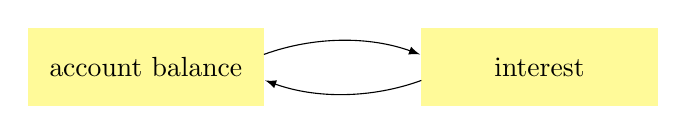
\begin{tikzpicture}
    \fill[color=yellow!40!white] (-4,2) rectangle (-1,3) node[pos=.5] {\color{black}account balance};
%    \draw (-1,2.5) -- (1,2.5);
    \fill[color=yellow!40!white] (1,2) rectangle (4,3) node[pos=.5] {\color{black}interest};
    \draw[-{latex}] (-1,2.66) arc (110:70:2.9);
    \draw[-{latex}] (1,2.33) arc (290:250:2.9);
\end{tikzpicture}	
\end{center}


\paragraph{Step 3.} Let us make the following assumptions:
\begin{itemize}
	\item We make one initial deposit into the account at time $n=0$.
	\item We don't make any more withdrawals or deposits.
	\item The only way the savings account balance changes is through the interest, which is the interest rate $p\%$ of the current balance.
\end{itemize}

\paragraph{Step 4.} We create the following model
$$ 
\begin{array}{ccccccl}
b_{n+1} & = & \big(\substack{\rm previous\\ \rm balance}\big) & + & {\rm interest} \\
b_{n+1}& =& b_n & + & \alpha \frac{p}{100} b_n & = & \left( 1 + \alpha \frac{p}{100}\right) b_n.
\end{array}
$$
	
\end{example}


\hfill

\newpage 
\submodule{Probability Models}

There are several circumstances that involve probabilities that can be modelled using difference equations.

Below is an example of one such circumstance.


\begin{example}

A gambler plays a game at a casino. The game is played one round at a time. 
\vfill

Each round, one of two things happens:
\begin{itemize}
\item The gambler wins \$1 with a probability of $q$
\item The gambler loses \$1 with a probability of $1-q$\\
\end{itemize}

The gambler will stop playing only if
\begin{itemize}
\item The gambler is ruined (bankrupt)
\item The gambler reaches $\$W$.\\
\end{itemize}

What is the probability $\pmb{p_n}$ that the player will be ruined if he starts gambling with $\$n$  ?	 \\


\paragraph{Step 2.} Mind map.
\begin{center}
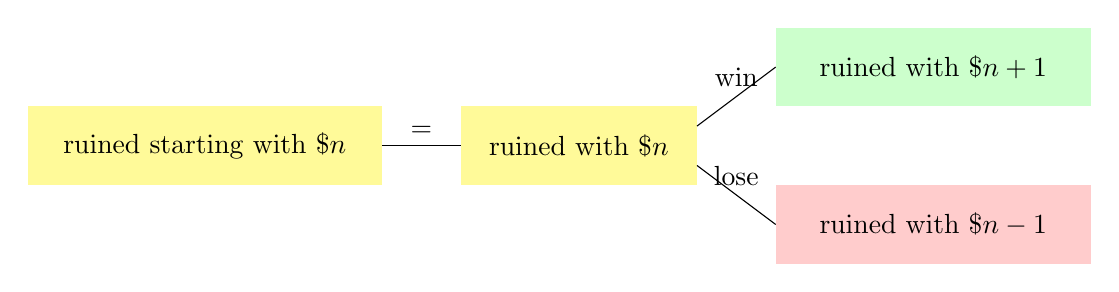
\begin{tikzpicture}
    \fill[color=yellow!40!white] (-4.5,2) rectangle (0,3) node[pos=.5] {\color{black}ruined starting with $\$n$};
    \draw (0,2.5) -- (1,2.5) node[pos=.5,above] {$=$};
    \fill[color=yellow!40!white] (1,2) rectangle (4,3) node[pos=.5] {\color{black}ruined with $\$n$};
    \draw (4,2.75) -- (5,3.5) node[pos=.5,above] {win};
    \fill[color=green!20!white] (5,3) rectangle (9,4) node[pos=.5] {\color{black}ruined with $\$n+1$};
    \draw (4,2.25) -- (5,1.5) node[pos=.5,above] {lose};
    \fill[color=red!20!white] (5,1) rectangle (9,2) node[pos=.5] {\color{black}ruined with $\$n-1$};
\end{tikzpicture}	
\end{center}


The two boxes on the left are very important. The crucial idea is to realize that it doesn't matter when the gambler has $\$n$. If s/he has $\$n$ at two different points in time, then the probability of becoming ruined is the same. \\

This mind map, shows us that we can relate $p_n$, $p_{n+1}$ and $p_{n-1}$.\\

The rest of the modelling will be left as a practice problem.

\end{example}


\begin{video}
\begin{itemize}
	\item \qrvideo{https://youtu.be/Rr2iSKlengg}
\end{itemize}	
\end{video}


\hfill


\submodule{Population Models}

We have modelled populations using differential equations. Populations can be modelled using both differential or difference equations. Which kind of equations to use depends on the goal of the model and the assumptions that we make. 

Below we'll see an example of a population model using difference equations.


\begin{example}

Model a population of mosquitoes, who reproduce at specific times of the year.

\paragraph{Step 1.} The goal is to model the population, so we define
\begin{itemize}
	\item $p(t) = $ population of mosquitoes at time $t$.
\end{itemize}



\paragraph{Step 2.} We create a mind map for this problem.

\begin{center}
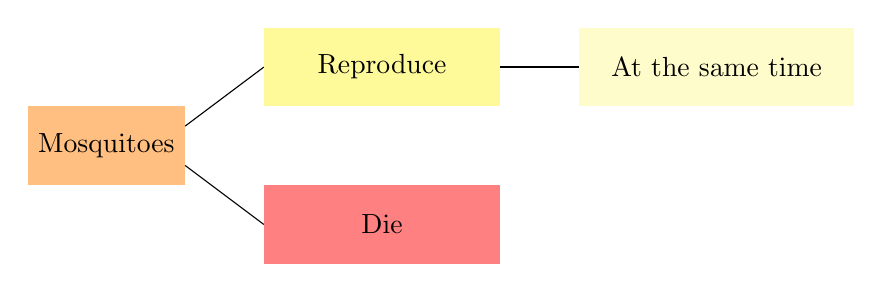
\begin{tikzpicture}
    \fill[color=orange!50!white] (-4.5,2) rectangle (-2.5,3) node[pos=.5] {\color{black}Mosquitoes};
    \draw (-2.5,2.75) -- (-1.5,3.5);
    \fill[color=yellow!40!white] (-1.5,3) rectangle (1.5,4) node[pos=.5] {\color{black}Reproduce};
    \draw (-2.5,2.25) -- (-1.5,1.5);
    \fill[color=red!50!white] (-1.5,1) rectangle (1.5,2) node[pos=.5] {\color{black}Die};
    \draw (1.5,3.5) -- (2.5,3.5);
    \fill[color=yellow!20!white] (2.5,3) rectangle (6,4) node[pos=.5] {\color{black}At the same time};
\end{tikzpicture}
\end{center}



\paragraph{Step 3.} Given that the mosquito population all reproduces at the same time, we don't need to track the population at all times $t$.

So we can assume that the mosquito population doesn't change (much) between seasons, and we change our objective function from $p(t)$ to $p_n$:
\begin{itemize}
	\item $p_n = $ population of mosquitoes at the beginning of season $n$.
\end{itemize}

We understand that mosquitoes die in between seasons, but in this model, we only count the deaths at the beginning of each season. \\

The next assumption is that the number of nymphs (baby mosquitoes) is proportional to the number of mosquitoes in the beginning of the season.

Similarly, the number of deaths is proportional to the number of mosquitoes in the beginning of the season. Also observe that mosquitoes only live for one season, which means that the proportionality constant $\mu > 1$.



\paragraph{Step 4.} So our model is
\begin{itemize}
	\item $p_n = $ population of mosquitoes at the beginning of season $n$.
	\item $p_{n+1} = r p_n - \mu p_n = (r-\mu)p_n$;
	\item $r = $ the average number of nymphs per per mosquito per season;
	\item $\mu = $ the average number of deaths per mosquito per season;
	\item $\mu > 1$, which means that each mosquito itself dies (at the end of the seasons if not earlier), but also some of its nymphs will die.
\end{itemize}

\end{example}

\begin{video}
\begin{itemize}
	\item \qrvideo{https://youtu.be/qmm9GPhA1MY}
	\item \qrvideo{https://youtu.be/j__Kredt7vY}
\end{itemize}	
\end{video}


	\newpage

\begin{exercises}

	Create a model for the following situations.
	\begin{problist}
	\prob You just took a loan to buy a car. You'll need to make fixed payments every period, and the bank will charge an interest on the amount you still owe every period.

		\begin{center}
			\includegraphics*[width=150pt]{images/module25-chirping-echo.pdf}
		\end{center}

	\prob A bird is chirping to find a mate. Unfortunately it is standing next to a cave which echoes its chirps. Consider the following:

 
			\begin{enumerate}[label={(P$_{\arabic*}$) } ]
			\item The bird chirps once every minute;
			\item The maximum volume the bird can chirp is $M$ dB;
			\item If it hears a chirp, then it chirps at a volume proportional to the volume of the chirp it heard times the difference between the maximum volume it is capable and the volume heard with constant $A \ \frac{1}{dB}$;
			\end{enumerate}



	\prob IBM just developed an new software that they wish to charge for usage. In this program, there is a parameter $n$ that you can choose to change how it performs:
			\begin{itemize}
			\item $n^2 = $ number of operations it takes to run the program;
	%		\item Each operation takes $10^{-3}$ seconds;
	%		\item The error of the result is inversely proportional to $n$, i.e., proportional to $\frac1n$;
			\item The profit IBM will make is $- \ln({\rm error})$ in Canadian dollars (negative means that IBM has to pay a penalty).
			\end{itemize}
	
			Model the profit that IBM makes. Remember to consider all sources of costs.
	
	\prob Let us study Engineering students at the University of Toronto. Find a model for the number of undergraduate students in the Engineering school at the University of Toronto and how they change from year to year. 

	\prob You are working for Canada Revenue Agency and the queue in the IRS complaints section is getting too large and lengthy. One way to solve this would be to stop collecting taxes, but that's not possible, so you are tasked with modelling the queue. 

			Model a queue on a typical weekday afternoon minute by minute. 
%			Here are some details about the queue:
%			\begin{itemize}
%			\item The average number of people joining the queue per minute is $\beta$.
%			\item On average, $\gamma\%$ of people in the queue are attended and leave the queue per minute.
%			\item Also on average $\mu\%$ of people in the queue give up waiting and leave the queue per minute.
%			\end{itemize}


	
	\prob Read the example above about the gambler's ruin. Finish creating a model for it.

	\prob A ball bouncing on the floor.
	
	\prob A person has some fever and takes tylenol every 4 hours. What is the concentration of tylenol in her bloodstream?
	
	\end{problist}
\end{exercises}

\end{module}



\begin{lesson}
	\Title{Modelling with Difference Equations}

	\Heading{Objectives}
	\begin{itemize}
		\item Bla
	\end{itemize}
	
	\Heading{Motivation} 

\end{lesson}



\begin{annotation}
\begin{goals}
	The effective annual interest rate is the interest rate with a compounding period of 1 year that gives the same result s the rate of $p\%$ compounded every $\alpha$ years.
\end{goals}
\end{annotation}
\question
	Let us expand on the economic example above.
	
	We put a certain amount of money in a savings bank account with an annual interest rate of $p\%$, and compounded at regular periods of $\alpha$ (in years). \\
	
	Even though we call $p\%$ the annual interest rate, because it is compounded during the year, at the end of the year the effective annual interest rate $p_{\rm eff}\%$ is actually higher.
	
	Calculate the effective interest rate $p_{\rm eff}\%$.


	

\bookonlynewpage


\question The goal of this quesiton is to try to understand the meaning of average lifespan.
\begin{annotation}
\begin{goals}
	\Goal{Pre-class question}
	The goal of this question is to prepare for calculating the average lifespan in the next page. \\

	Not to do in lecture. Assign to students to solve at home before.
\end{goals}
\end{annotation}
\begin{parts}
	\item Consider a small tribe, where the people in there died at the ages:		
		\begin{graybox}
		\begin{center}
			42, 56, 46, 52, 5, 103, 47, 67, 67, 85, 57, 42, 47, 67, 46, 42, 5, 46, 57, 42.
		\end{center}
		\end{graybox}
		What is the average lifespan of this tribe's population? %51.05

	\item  Consider another small tribe, where people recorded their lifespans differently. Below is a table with the percentage of the population that died at each age:
		\begin{graybox}
		\begin{center}
		\begin{tabular}{c||c|c|c|c|c|c|c}
			\textbf{Percentage of population}
				& 2\% & 5\% & 9\% & 9\% & 16\% & 22\% & 37\% \\ \hline
			\textbf{Age at death}
				& 98 & 82 & 71 & 66 & 61 & 53 & 48\\
		\end{tabular}
		\end{center}
		\end{graybox}
		What is the average lifespan of this tribe's population? %57.57
\end{parts}
 

\vfill



\bookonlynewpage



\begin{annotation}
\begin{goals}
	Some hints:
	\begin{itemize}
		\item individual dying during season $k$ $\Leftrightarrow$ lifespan $= k$ seasons
		\item From previous two exercises, deduce that: average lifespan $=$ expected value of lifespan $\ell = E$:
		$$ E = \sum_{k=0}^\infty k \ell(k) $$
		\item $\displaystyle \sum_{k=1}^\infty k r^k = \frac{r}{(1-r)^2}$ for $|r|<1$.
		\item End result should be $\frac1\mu$.
\end{itemize}	
\end{goals}
\end{annotation}
\question
	Given a population with
	\begin{itemize}
		\item $\mu=$ probability that an individual will die between two seasons.
	\end{itemize}
\begin{parts}
	\item Define the following quantity
	\begin{itemize}
		\item $P(k)=$probability that an individual born at season $0$ is alive at the beginning of season $k$.
	\end{itemize}
	Find a model for $P(k)$.

	\item What is the probability of the individual dying during the k$^{\rm th}$ season?
	\item What is the average lifespan of an individual in this population?
\end{parts}




\bookonlynewpage


\question
	Consider a population of special rabbits. Once a pair of rabbits is born, they grow and one year later they are still immature. But two years after they are born they give birth to another pair of rabbits.
	
\begin{annotation}
	\begin{goals}
		If there is time, students should show that the Fibonacci sequence does indeed match the number of rabbits.
	\end{goals}
\end{annotation}
	Model this population of rabbits.	

	


\bookonlynewpage


\question
	Consider another population of rabbits. This is the lifecycle of a pair of rabbits:
	\begin{enumerate}[start=0,label=(year \arabic*)]
		\item Born
		\item Immature (no babies)
		\item Young Adult (1 pairs of babies)
		\item Adult (1 pair of babies)
		\item Old (no babies)
		\item Die
	\end{enumerate}	
\begin{annotation}
	\begin{goals}
		Students might try to find a pattern. 
		
		It is possible, but very difficult.
		
		Hint: Use a system of difference equations. \\
		
		In core exercise \ref{rabbitscomplicatedproof}, the students are asked to prove the formula.
	\end{goals}
\end{annotation}
	
	Model this population of rabbits.
	
	




\standardonlynewpage
%
%
%
%%%%%%%%%%%%%%%%%%%%%%%%%%%%%%%
%%
%%  MODULE - Models with probabilities
%%
%%%%%%%%%%%%%%%%%%%%%%%%%%%%%%%
%
%
%
%\begin{module}{Models with probabilities}
%	\label{diff:prob}
%
%	\input{modules/module23-diff-prob.tex}
%	\input{modules/module23-diff-prob-exercises.tex}
%\end{module}
%
%
%
%\begin{lesson}
%	\Title{Models with probabilities}
%
%	\Heading{Objectives}
%	\begin{itemize}
%		\item Bla
%	\end{itemize}
%	
%	\Heading{Motivation} 
%
%\end{lesson}
%
%
%\newpage
%
%\question
%	Core Exercise with several parts
%\begin{parts}
%	\item Part 1
%	\item Part 2
%\end{parts}
%
%\bookonlynewpage
%
%
%\question
%	One more core exercise
%
%




%
%%%%%%%%%%%%%%%%%%%%%%%%%%%%%%%
%%
%%  MODULE - Models for Two or More Interconnected Quantities
%%
%%%%%%%%%%%%%%%%%%%%%%%%%%%%%%%
%
%
%
%\begin{module}{Models for Two or More Interconnected Quantities}
%	\label{diff:sys}
%
%	\input{modules/module26-diff-sys.tex}
%	\input{modules/module26-diff-sys-exercises.tex}
%\end{module}
%
%
%
%\begin{lesson}
%	\Title{Models for Two or More Interconnected Quantities}
%
%	\Heading{Objectives}
%	\begin{itemize}
%		\item Bla
%	\end{itemize}
%	
%	\Heading{Motivation} 
%
%\end{lesson}
%
%
%\newpage
%
%\question
%	Core Exercise with several parts
%\begin{parts}
%	\item Part 1
%	\item Part 2
%\end{parts}
%
%\bookonlynewpage
%
%
%\question
%	One more core exercise
%
%

%%%%%%%%%%%%%%%%%%%%%%%%%%%%%%
%
%  MODULE - Analysis of Difference Equations
%
%%%%%%%%%%%%%%%%%%%%%%%%%%%%%%



\begin{module}{Analysis of Difference Equations}
	\label{diff:analysis}

	In this module you will learn
\begin{itemize}
	\item some ways to analyze models with difference equations
\end{itemize}

\hfill \\




We have seen some different types of models involving difference equations. we have also seen a few different ways to solve them.

We will now see an example of how we can analyze a difference equation.



\begin{example}

Consider the following model for the number of Mathematics students at a University:
\begin{itemize}
\item $e_k = $ number of students in the year $2020+k$;
\item $a_k = $ number of students admitted to the first year;
\item $g = $ percentage of students that graduate every year;
\item $q = $ percentage of students that quit the Mathematics program  every year. \\

\item $e_{k+1} = e_k + a - g e_k - q e_k$
\end{itemize}

\end{example}

\hfill

\begin{center}
\textbf{\color{cyan}
Finding the equilibrium point(s)
}
\end{center}


What is the equilibrium number of students $E$? This means that we are looking for a solution that remains constant $e_{k+1}=e_k = E$.

$$
E = E + a - (g+q)E
\quad \Leftrightarrow\quad
	E = \frac{a}{g+q}
$$

This is the value that the department should strive for, since it would remain stable.


%\newpage
\hfill

\begin{center}
\textbf{\color{cyan}
Numerical approximations
}
\end{center}


For models with difference equations, we don't need numerical methods, since the recursive definition of the sequence is already a numerical method in itself.

We can follow the same approach however and run some numbers and with different values for the parameters to gain some intuition on the solutions.

\begin{center}
\begin{tabular}{cc}
\includegraphics*[width=150pt]{images/module26-stud-above.png}
	& \includegraphics*[width=150pt]{images/module26-stud-below.png} \\
$e_0 > E$ 
	& $e_0 < E$
\end{tabular}
\end{center}
 

\begin{graybox}
You can access this simulation here:
\begin{itemize}
	\item \qrvideo{https://www.desmos.com/calculator/wv3oxrjvrz}
\end{itemize}	
\end{graybox}


\hfill

\begin{center}
\textbf{\color{cyan}
Qualitative evolution of quantities
}
\end{center}


Let us now look at what happens if the situation is not in equilibrium. The numerical study above, gives some intuition about the behaviour of solutions. 

Let us assume that $e_k  > E$. Then
\begin{align*}
e_{k+1}
	& = e_k (1-g-q) + a \\
	& > E (1-g-q) + a \tag{see note below} \\
	& = E - E(g+q)+a \\
	& = E - \frac{a}{g+q}(g+q) + a\\
	& = E
\end{align*}

\begin{graybox}
\textbf{Note. } This step is only true if $E$ and $1-g-q>0$. (Why?) \\

It's clear that $E$ should be positive, since it is a number of students. \\

The other quantity is not so obvious: \quad $g+q < 1$ ?

In fact, $g+q$ is the fraction of students that graduate or quit the Mathematics program, so it can't exceed 1! (Why?)
\end{graybox}


We conclude that if $e_k > E$, then $e_{k+1}>E$. This means that if the number of students starts above the equilibrium, then it will always stay above it.\\

But will the number of students keep increasing without bound or will it converge to a number?\\

Let us check:
\begin{align*}
e_{k+1} - e_k
	& = a - e_k (g+q) \\
	& < a - E (g+q) \\
	& = a - \frac{a}{g+q} (g+q) \\
	& = 0
\end{align*}

So we conclude that 
$$
e_{k+1} - e_k < 0 \quad \Leftrightarrow \quad e_{k+1} < e_k,
$$
so the number of students will decrease.

Our conclusion is that if $e_k > E$, then $e_{k+1} \in [E, e_k]$:
\begin{center}
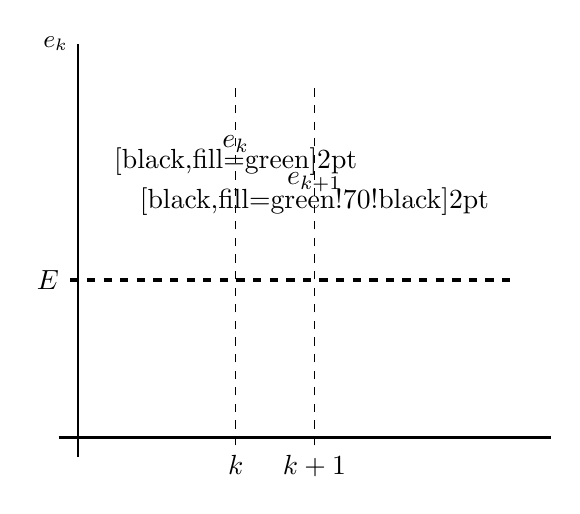
\begin{tikzpicture}
  \draw[thick,-{\seta}] (-0.25,0) -- (6,0) ;%node[above] {\small $k$};
  \draw[thick,-{\seta}] (0,-0.25) -- (0,5) node[left] {\small $e_k$};
%  \draw[] (2,0) node[below] {$k$};
  \draw[dashed] (2,-0.1) node[below] {$k$} -- (2,4.5);
%  \draw[] (3,0) node[below] {$k+1$};
  \draw[dashed] (3,-0.1) node[below] {$k+1$} -- (3,4.5);
  \draw[ultra thick,dashed] (-0.1,2) node[left] {$E$} -- (5.5,2)  ;
%
  \draw (2,3.5) node {\tikzcircle[black,fill=green]{2pt}} node[above] {$e_{k}$};
  \draw (3,3) node {\tikzcircle[black,fill=green!70!black]{2pt}} node[above] {$e_{k+1}$};
\end{tikzpicture}
\end{center}


Similarly, if $e_k < E$, we can conclude that $e_{k+1} \in [e_k,E]$:
\begin{center}
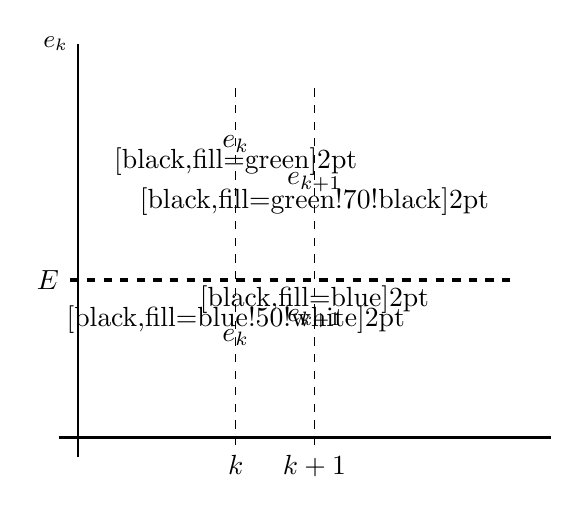
\begin{tikzpicture}
  \draw[thick,-{\seta}] (-0.25,0) -- (6,0) ;%node[above] {\small $k$};
  \draw[thick,-{\seta}] (0,-0.25) -- (0,5) node[left] {\small $e_k$};
%  \draw[] (2,0) node[below] {$k$};
  \draw[dashed] (2,-0.1) node[below] {$k$} -- (2,4.5);
%  \draw[] (3,0) node[below] {$k+1$};
  \draw[dashed] (3,-0.1) node[below] {$k+1$} -- (3,4.5);
  \draw[ultra thick,dashed] (-0.1,2) node[left] {$E$} -- (5.5,2)  ;
%
  \draw (2,3.5) node {\tikzcircle[black,fill=green]{2pt}} node[above] {$e_{k}$};
  \draw (3,3) node {\tikzcircle[black,fill=green!70!black]{2pt}} node[above] {$e_{k+1}$};
  \draw (2,1.5) node {\tikzcircle[black,fill=blue!50!white]{2pt}} node[below] {$e_{k}$};
  \draw (3,1.75) node {\tikzcircle[black,fill=blue]{2pt}} node[below] {$e_{k+1}$};
\end{tikzpicture}
\end{center}


So we can see that the sequence $e_k$ will be approaching $E$, so we can say that the \emph{equilibrium is stable}.







\hfill

\begin{center}
\textbf{\color{cyan}
Limiting behaviour of the solutions
}
\end{center}



From our previous analysis, we can see that it looks like 
$$
\lim_{k \to \infty} e_k = E.
$$

But we didn't prove this yet. It could be that the sequence converges to some other value. 

To show this, we would need to define a new sequence $x_k = e_k-E$, assume that it has the form $x_k = C r^k$ and then obtain a characteristic equation for $r$:
$$
r = 1-g-q \in (0,1),
$$
so $x_k = C r^k$ and 
$$
\lim_{k \to \infty} x_k = 0
\quad \Leftrightarrow \quad
	\lim_{k \to \infty} e_k = E.
$$

So we now know that the number of students will converge monotonically to the equilibrium.








	\newpage 

\begin{exercises}

		\begin{problist}
	
	\prob Consider the following discrete population model:
	\begin{itemize}
		\item $p_k=$ population at the beginning of season $k$
		\item $R = $ basic reproduction value for the population
		\item $K= $ carrying capacity 
		\item $\displaystyle p_{k+1}=p_k + R p_k\left(1-\frac{p_k}{K}\right)$
	\end{itemize}
	
	\begin{enumerate}
		\item Define:
		\begin{itemize}
			\item $\mu = 1+R$,
			\item $\displaystyle x_k = \frac{R}{1+R} \frac{p_k}{K}$.
		\end{itemize}
		Show that $x_{k+1} = \mu x_k (1-x_k)$.
		\item What are the equilibrium values for $x_k$?
	%	$$
	%	E = 1 - \frac1\mu = \frac{mu-1}{\mu}
	%	$$
	
		\item Take $R=1, \mu=2$. Compare this model with the continuous logistic model.
		\item In the continuous model, solutions cannot cross the equilibrium. 
		Change the value of $R,\mu$ and show that in this discrete model, solutions can cross the equilibrium.
		
		\item Take $R=3, \mu=4$ (constants for influenza virus). Below is a graph with $\color{green!70!black}x_0 = 0.1$ and $\color{blue!85!black}x_0=0.101$.
	
			\begin{center}
				\includegraphics*[width=150pt]{images/module26-logistic.png}
			\end{center}
		
			Which conclusions do you take from this graph?
			
		\item Take $x_0=\frac12$. What happens to $x_k$ as $k$ gets larger and larger: does it remain bounded, or does it converge to $\pm \infty$? Check for different values of $\mu$.

		\item You'll need to program for this exercise. Now allow complex values for $\mu \in \mathbb{C}$. In a graph, mark the values of $\mu \in \C$, for which $x_n$ does not diverge to infinity.
		
%		\includegraphics*[width=150pt]{images/module26-mandelbrot.png}
		
	\end{enumerate}

\begin{annotation}
\begin{goals}
	\begin{itemize}
	\item[1.] You can skip the first part and tell students to do it at home.
	
	\item[3.] For the comparison part, notice how the model is very similar in the way it looks. If you run the model it also behaves very similarly.

	\qrvideo{https://www.desmos.com/calculator/zxk8udxmac}
	
	\item[4.] For the last part, for $\mu=3$, solutions oscillate but converge to equilibrium
	\item[5.] For the last part, for $\mu=4$, $x_0=0.1$ and $x_0=0.101$ gives completely different solutions. Chaotic behaviour. So need to be careful analyzing nonlinear difference equations.
	
		\qrvideo{https://www.desmos.com/calculator/e656u8n4vt}
	\end{itemize}
\end{goals}	
\end{annotation}

	

	

	\prob Consider the model for a queue:
	\begin{itemize}
		\item $q_n=$ number of people waiting in the queue at minute $n$;
		\item $\gamma=$ fraction of the people waiting that are attended each minute;
		\item $\mu=$ average number of people that give up waiting in the queue per minute;
	\end{itemize}

	\begin{enumerate}
		\item First, let us find out a very bad scenario for the queue. Find a number of initial people in the queue $q_0$ such that the size of the queue will never change.
		\item Let 
			\begin{itemize}
				\item $p_k=$ probability that a person who joined the queue at time $k=0$ will still be waiting after $k$ minutes.
			\end{itemize}
			Is $p_k$ increasing, decreasing, or not monotone?
		\item The probability that someone waited exactly $k$ minutes is $p_{k}-p_{k+1}$.
			Find another expression for $p_{k}-p_{k+1}$ without using $p_k$.
		\item The expected waiting time in the queue is given by the ``law'':
			
			\hspace{-.05\textwidth}\framebox{
			\begin{minipage}{.4\textwidth}
			The expected waiting time is the weighted average of the possible waiting times, where the weights are the probability of waiting that exact amount of time.
			\end{minipage}}
			
		Find the expected waiting time for this queue.
	\end{enumerate}
	
	
	
	
	
	\prob 	Two computers are facing each other on video conferencing software. The first computer makes a sound and every fraction of a second, the other computer reproduces the sound.
	
	Consider the following model for the microphone feedback:
	\begin{itemize}
		\item $v_n =$ volume produced by the first computer (in dB) for the $n$ iteration;
		\item $e=$ fraction of the original volume reproduced by the second computer;
		\item $M=$ maximum volume that first computer can produce (in DB). \\

		\item $v_{n+1} = e v_n \left( \frac{M - e v_n}{M}+1\right)$.
	\end{itemize}
	
	\begin{enumerate}
		\item What is the initial volume that will just cause the following iterations to be the same?


		\item Find a condition on $e$ that allows for the previous situation to occur.

%v>0 iff 
%v<M iff 

		\item Assume $e \in (0,1)$. What happens if the initial volume is softer than the equilibrium? What happens if the initial volume is louder than the equilibrium?
		\item Assume $e>1$. What happens if the initial volume is softer than the equilibrium? What happens if the initial volume is louder than the equilibrium?

		\item Assume $e=\frac85$. Sketch a graph of the solution.
		
%		\begin{itemize}
%			\item $v_0 = M$	
%			\item $v_1 = \frac{16}{25}M$
%			\item $v_2 = \frac85 \frac{16}{25}M \frac{122}{125} \approx M$
%		\end{itemize}

		What is the behaviour of the solution as $n$ gets larger?
		
		\item Assume $e=\frac{1+\sqrt{5}}{2}$ the golden ratio. Is there an initial volume that gives a periodic solution: $v_0=v_2=v_4,v_5=\cdots$ and $v_1=v_3=v_5=v_7=\cdots$?
	
	\end{enumerate}
	
\begin{annotation}
\begin{goals}
	For 2, remember that the first computer has to be able to produce the sound: $v_n < M$, and the sound needs to be audible $v_n>0$.
\end{goals}	
\end{annotation}


		
	\end{problist}
\end{exercises}
\end{module}



\begin{lesson}
	\Title{Analysis of Difference Equations}

	\Heading{Objectives}
	\begin{itemize}
		\item Bla
	\end{itemize}
	
	\Heading{Motivation} 

\end{lesson}




\question 
	Consider the following difference equation:
		$$u_{k+1} = a(u_k - b)$$

	\begin{parts}
		\item What is the equilibrium solution?
		\item Are there 2-periodic solutions? I.e. satisfying
\begin{annotation}
	\begin{goals}
		\begin{itemize}
			\item In the calculations for .2, there is a step that involves a division by $(1-a^2)$, so it can only be done for $a \neq \pm 1$.
			\item The final result for .2 is:
			\begin{align*}
				a \neq \pm1. & \quad {\rm periodic} \Rightarrow u_0 = \frac{ab}{a-1} \quad & \Rightarrow & 1-{\rm periodic} \\
				a = 1. & \quad {\rm periodic} \Rightarrow b=0  & \Rightarrow & 1-{\rm periodic} \\
				a = -1. & \quad {\rm periodic} \Rightarrow b=0  & \Rightarrow & 2-\text{periodic if } u_0\neq 0
			\end{align*}
		\end{itemize}
	\end{goals}
\end{annotation}
		\begin{itemize}
			\item $v_0=v_2=v_4=v_6=\cdots$
			\item $v_1=v_3=v_5=v_7=\cdots$
			\item $v_0\neq v_1$
		\end{itemize} 
		\item What happens to the solutions for different values of $a$?
		\item What happens to the solutions for different values of $b$?
	\end{parts}






\bookonlynewpage

\question
	Consider a drunkard that is walking randomly near a cliff.

	\hfill \includegraphics*[width=250pt]{images/module26-drunk.pdf}
	\vspace{-70pt}

	\begin{minipage}{.9\textwidth}
		Consider this model for the drunkard's chance of getting to safety from falling off the cliff:
		\begin{itemize}
			\item $q$ is the probability that the drunkard will step towards safety;
			\item $1-q$ is the probability that the drunkard will step towards the cliff;
			\item $p_n=$ probability that the drunkard will get to safety if he is in step number $n$; 
			\item The drunkard will stop moving if he gets to safety (step $W$) or if he falls out of the cliff (step $0$); \\
	
			\item $p_n = q p_{n+1} + (1-q) p_{n-1}$. \\
		\end{itemize}
	\end{minipage}

	
\begin{annotation}
	\begin{goals}
		Question .3 is purposefully ambiguous about symmetry. What kind of symmetry is there? Is there any?
	\end{goals}
\end{annotation}
	\begin{parts}
		\item Is $p_n$ increasing or decreasing?
		\item What is $p_0$? What is $p_W$?
		\item Let $q=\frac12$. What is $p_{W/2}$? Is $p_n$ symmetric around $n=\frac{w}{2}$?
		\item Let $q>\frac12$. Is $p_{W/2} > \frac12$? Is $p_{W/2} < \frac12$? 
		\item How do solutions for $q=\alpha$ and $q=1-\alpha$ compare?
	\end{parts}


	
\bookonlynewpage

\hfill

\bookonlynewpage


\begin{minipage}{.45\textwidth}
\question \label{rabbitscomplicatedproof}
	Consider a population of rabbits with the following lifecycle:
	\begin{enumerate}[start=0,label=(year \arabic*)]
		\item Born
		\item Immature (no babies)
		\item Young Adult (1 pair of babies)
		\item Adult (1 pair of babies)
		\item Old (no babies)
		\item Die \\[5pt]
	\end{enumerate}	
	
\end{minipage}
\qquad
\begin{minipage}{.45\textwidth}
	Consider the definitions:
	\begin{itemize}
		\item We start with 1 pair of newborn rabbits in year 0;
		\item $r_n=$ number of pairs of rabbits alive during year $n$;
		\item $i_k=$ number of immature pairs;
		\item $y_k=$ number of young adult pairs;
		\item $a_k=$ number of adult pairs;
		\item $o_k=$ number of old pairs.
	\end{itemize}

\end{minipage}

	\begin{parts}
		\item Show that $b_k=b_{k-2}+b_{k-3}$.
		\item Show that $y_{k+1}=o_{k}+o_{k+1}$.
		\item Show that $r_{n} = r_{n-2}+r_{n-3}$.
	\end{parts}

\begin{annotation}
\begin{goals}
$$
r_k 
	= {\color{magenta}r_{k-1}-o_{k-1}}+{\color{blue}b_k}
$$

On the other hand, 
$$
\color{magenta}
r_{k-1}-o_{k-1}
  = b_{k-2} + 2 y_{k-2} + a_{k-2} 
  = r_{k-2} + y_{k-2} - o_{k-2}
$$
and
$$
\color{blue}
b_k 
  = b_{k-2}+b_{k-3}
  = y_{k-3} + a_{k-3} + b_{k-3}
  = r_{k-3} - o_{k-3}
$$

So we have
$$
r_k = {\color{magenta}r_{k-2} + {\color{black}\not} y_{k-2} - {\color{black}\not} o_{k-2}} + {\color{blue}r_{k-3} - {\color{black}\not}o_{k-3}}
= r_{k-2} + r_{k-3}
$$
\end{goals}
\end{annotation}	

	
	

\standardonlynewpage

%
%
%%%%%%%%%%%%%%%%%%%%%%%%%%%%%%%
%%
%%  MODULE - Nonlinear Models
%%
%%%%%%%%%%%%%%%%%%%%%%%%%%%%%%%
%
%
%
%\begin{module}{Nonlinear Models}
%	\label{diff:nonlinear}
%
%	In this module you will learn
\begin{itemize}
	\item some nonlinear models
	\item some of the difficulties of studying nonlinear models
\end{itemize}

\hfill \\


%	\begin{exercises}

	\begin{problist}
	\prob Show that all autonomous differential equations are separable.

	\end{problist}
\end{exercises}

%\end{module}
%
%
%
%\begin{lesson}
%	\Title{Nonlinear Models}
%
%	\Heading{Objectives}
%	\begin{itemize}
%		\item Bla
%	\end{itemize}
%	
%	\Heading{Motivation} 
%
%\end{lesson}
%
%
%\newpage
%
%\question
%	Core Exercise with several parts
%\begin{parts}
%	\item Part 1
%	\item Part 2
%\end{parts}
%
%\bookonlynewpage
%
%
%\question
%	One more core exercise
%
%








%
%
%%%%%%%%%%%%%%%%%%%%%%%%%%%%%%%%%%%%%%%%%%%%%%%%%%%%%%%%%%%%%%%%%%%%%%%%%
%%
%%		Jason's Linear Algebra Book
%%
%%%%%%%%%%%%%%%%%%%%%%%%%%%%%%%%%%%%%%%%%%%%%%%%%%%%%%%%%%%%%%%%%%%%%%%%%
%
%\newpage
%
%\hfill
%
%
%%%%%%%%%%%%%%%%%%%%%%%%%%%%%%%%%%%%%%%%%%%%%%%%%%%%%%%%%%%%%%%%%%%%%%%%
%
%		LINEAR ALGEBRA
%
%%%%%%%%%%%%%%%%%%%%%%%%%%%%%%%%%%%%%%%%%%%%%%%%%%%%%%%%%%%%%%%%%%%%%%%%


\begin{topic}[Linear Algebra]

\end{topic}


\newpage


\begin{module}
	\Title{Linear Combinations}

	\Heading{Textbook} Section 1.1

	\Heading{Objectives}
	\begin{itemize}
		\item Internalize vectors as geometric objects representing displacements.

		\item Use column vector notation to write vectors.

		\item Relate points an vectors and be able to interpret a point as
			a vector and a vector as a point.

		\item Solve simple equations involving vectors.
	\end{itemize}

	\Heading{Motivation} Students have differing levels of experience with vectors.
	We want to establish a common notation for vectors and use vector notation
	along with algebra to solve simple questions. E.g., ``How can I get to location
	$A$ given that I can only walk parallel to the lines $y=4x$ and $y=-x$?''


	\begin{annotation}
		\begin{notes}
			\begin{itemize}
			\item
			We will use the language \emph{component of $\vec v$ in
			the direction $\vec u$} in the future and it will be a \emph{vector}.
			For this reason, try to refer to the entries of a column
			vector as \emph{coordinates} or \emph{entries} instead of components.

			\item
			Though we will almost exclusively use
			column vector notation in this course, students should be able to parse
			questions phrased in terms of row vectors.
			\end{itemize}
		\end{notes}
	\end{annotation}
	
	We will use column vector notation and the idea of equating
	coordinates in order to solve problems.

\end{module}


\section*{Task 1.1: The Magic Carpet Ride}
\addcontentsline{toc}{subsection}{Task 1.1: The Magic Carpet Ride}


\begin{annotation}
	\begin{goals}
		\Goal{Hands-on experience with vectors as displacements.}
		\begin{itemize}
			\item Internalize vectors as geometric objects representing
				displacements.

			\item Use column vector notation to write vectors.

			\item Use pre-existing knowledge of algebra to answer vector
				questions.
		\end{itemize}
	\end{goals}
	\begin{notes}

		\begin{itemize}
			\item There are many ways to solve this problem.
				Some students
				might start with equations. After they use their
				equations to solve the problem, make them draw a picture
				and come up with a graphical solution.

			\item When the students start coming up with vector equations,
				give them the vocabulary of \emph{linear
				combinations}
				and \emph{column vector notation}.
		\end{itemize}
	\end{notes}
\end{annotation}
You are a young traveler, leaving home for the first time. Your parents
want to help you on your journey, so just before your departure, they give you two
gifts. Specifically, they give you two forms of transportation: a hover board and
a magic carpet. Your parents inform you that both the hover board and the magic carpet
have restrictions in how they operate:

\begin{minipage}{\textwidth}
	\vspace{.5cm}
	\begin{wrapfigure}{l}{1in}
	\vspace{-.8cm}
	
\includegraphics[width=1in]{images/HoverBoard-small.png}
	\end{wrapfigure}

	We denote the restriction on the hover board's movement by the vector
	$\mat{3 \\1}$. By this we mean that if
	the hover board traveled ``forward'' for one hour, it would move along a
	``diagonal'' path that would result in a displacement of 3 miles East and
	1 mile North of its starting location.
\end{minipage}

\begin{minipage}{\textwidth}
	\vspace{.5cm}
	\begin{wrapfigure}{l}{1in}
	\vspace{-.8cm}
	
\includegraphics[width=1in]{images/MagicCarpet-small.png}
	\end{wrapfigure}

	We denote the restriction on the magic carpet's movement by the vector
	$\mat{1 \\2 }$. By this we mean that if the
	magic carpet traveled ``forward'' for one hour, it would move along a
	``diagonal'' path that would result in a displacement of 1 mile East and
	2 miles North of its starting location.
\end{minipage}

\lfoot{\footnotesize Drawings by \url{@DavidsonJohnR} (twitter)}

\vspace{10mm}

% Scenario Section
\textbf{Scenario One: The Maiden Voyage}

Your Uncle Cramer suggests that your first adventure should be to go visit
the wise man, Old Man Gauss. Uncle Cramer tells you that Old Man Gauss
lives in a cabin that is 107 miles East and 64 miles North of your home.

\vspace{5mm}

\textbf{Task:}
\par
Investigate whether or not you can use the hover board and the magic
carpet to get to Gauss's cabin. If so, how? If it is not possible to
get to the cabin with these modes of transportation, why is that the case?

%\vspace{5mm}
% As a group, state and explain your answer(s) on the group whiteboard. Use
% the vector notation for each mode of transportation as part of your
% explanation and use a diagram or graphic to help illustrate your
% point(s).


\begin{module}
	\Title{Linear Combinations}

	\Heading{Textbook}
	Section 1.2

	\Heading{Objectives}
	\begin{itemize}
		\item Set up and solve vector equations $a\vec v+b\vec u=\vec w$. The solving
			method may be ad hoc.
		\item Use set notation and set operations/relations $\cup$, $\cap$, $\in$, $\subseteq$.
		\item Translate between set-builder notation and words in multiple ways.
	\end{itemize}

	\Heading{Motivation}
	We revisit questions about linear combinations more formally and generate a need for
	algebra. The algebra we do to solve vector equations will become algorithmic when
	we learn row reduction, but at the moment, any method is fine.

	\begin{annotation}
		\begin{notes}
			You will have a mix of MAT135/136 and MAT137 students.
			The MAT137 students will be doing logic and sets in their
			class. The MAT135 students won't. Make sure not to leave them
			behind!
		\end{notes}
	\end{annotation}
	As we talk about more complex objects, we need precise ways to talk about
	groups of vectors. I.e., we need sets and set-builder notation. This preview of set-builder
	notation will take some of difficulty away when we define span as a set of vectors.

	In this course we will be using formal and precise language. Part of this module
	is that there are multiple correct ways (and multiple incorrect ways) to use formal
	language. Gone are the days of ``there's only one right answer and it is 4''!

\end{module}


\section*{Task 1.2: The Magic Carpet Ride, Hide and Seek}
\addcontentsline{toc}{subsection}{Task 1.2: The Magic Carpet Ride, Hide and Seek}


\begin{annotation}
	\begin{goals}
		\Goal{Address an existential question involving vectors: ``Is it possible
		to find a linear combination that does\ldots?''}

		The goal of this problem is to
		\begin{itemize}
			\item Formalize geometric questions using the language of vectors.
			\item Find both geometric and algebraic arguments to support the same
				conclusion.
			\item Establish what a ``negative multiple'' of a vector should be.
		\end{itemize}
	\end{goals}
	\begin{notes}
		\begin{itemize}
			\item Both \emph{yes} and \emph{no} are valid answers to
				this question depending on whether you are allowed
				to go backwards. Establish that ``negative'' multiples of
				a vector mean traveling backwards along that vector.
			\item This problem can be solved with algebra by finding a formula
				for the coefficients for an arbitrary position or with geometry,
				with arguments eventually hinging on the fact that non-parallel
				lines do not intersect.
		\end{itemize}
	\end{notes}
\end{annotation}
You are a young traveler, leaving home for the first time. Your parents
want to help you on your journey, so just before your departure, they give
you two gifts. Specifically, they give you two forms of transportation:
a hover board and a magic carpet. Your parents inform you that both the
hover board and the magic carpet have restrictions in how they operate:



\begin{minipage}{\textwidth}
	\vspace{.5cm}
	\begin{wrapfigure}{l}{1in}
	\vspace{-.8cm}
	
\includegraphics[width=1in]{images/HoverBoard-small.png}
	\end{wrapfigure}

	We denote the restriction on the hover board's movement by the vector
	$\mat{3 \\1}$. By this we mean that if
	the hover board traveled ``forward'' for one hour, it would move along a
	``diagonal'' path that would result in a displacement of 3 miles East and
	1 mile North of its starting location.
\end{minipage}

\begin{minipage}{\textwidth}
	\vspace{.5cm}
	\begin{wrapfigure}{l}{1in}
	\vspace{-.8cm}
	
\includegraphics[width=1in]{images/MagicCarpet-small.png}
	\end{wrapfigure}

	We denote the restriction on the magic carpet's movement by the vector
	$\mat{1 \\2 }$. By this we mean that if the
	magic carpet traveled ``forward'' for one hour, it would move along a
	``diagonal'' path that would result in a displacement of 1 mile East and
	2 miles North of its starting location.
	\vspace{1cm}
\end{minipage}



\textbf{Scenario Two: Hide-and-Seek}

Old Man Gauss wants to move to a cabin in a different location. You are
not sure whether Gauss is just trying to test your wits at finding him
or if he actually wants to hide somewhere that you can't visit him.

\vspace{5mm}

\textbf{Are there some locations that he can hide and you cannot reach him
with these two modes of transportation?}

Describe the places that you
can reach using a combination of the hover board and the magic carpet and
those you cannot. Specify these geometrically and algebraically. Include
a symbolic representation using vector notation. Also, include a convincing
argument supporting your answer.

%\vspace{5mm} \par \textbf{Use your
%group's whiteboard as a space to write out our work as your work together
%on this problem.}



\pagestyle{siefken}

\section*{Sets and Set Notation}
\vspace{-.5cm}

	\begin{definition}[Set]
		A \emph{set} is a (possibly infinite) collection of items
		and is notated with curly braces (for example, $\{1,2,3\}$ is
		the set containing the numbers 1, 2, and 3).  We call the items in
		a set \emph{elements}.

		If $X$ is a set and $a$ is an element of $X$, we may write $a\in X$,
		which is read ``$a$ is an element of $X$.''

		If $X$ is a set, a \emph{subset} $Y$ of $X$ (written $Y\subseteq X$)
		is a set such that every element of $Y$ is an element of $X$. Two sets are
		called \emph{equal} if they are subsets of each other (i.e., $X=Y$ if
		$X\subseteq Y$ and $Y\subseteq X$).

		We can define a subset using \emph{set-builder notation}.
		That is, if $X$ is a set, we can define the subset
		\[
			Y= \Set*{a\in X \given \text{some rule involving }a},
		\]
		which is read ``$Y$ is the set of $a$ in $X$ {\bf such that} some rule
		involving $a$ is true.''  If $X$ is intuitive, we may omit it and
		simply write $Y=\{a:\text{some rule involving }a\}$.  You may equivalently
		use ``$|$'' instead of ``$:$'', writing $Y=\{a\,|\,\text{some rule involving }a\}$.
	\end{definition}

	\begin{definition}
		Some common sets are
		\begin{itemize}
			\item[] $\N=\Set{\text{natural numbers}} = \Set{\text{non-negative whole numbers}}$.
			\item[] $\Z=\Set{\text{integers}} = \Set{\text{whole numbers, including negatives}}$.
			\item[] $\R=\Set{\text{real numbers}}$.
			\item[] $\R^n=\Set{\text{vectors in $n$-dimensional Euclidean space}}$.
		\end{itemize}
	\end{definition}


	\question
	\begin{annotation}
		\begin{goals}
			\Goal{Practice reading sets and set-builder notation.}

			The goal of this problem is to
			\begin{itemize}
				\item Become familiar with $\in$, $\subseteq$, and $=$ in
					the context of sets.
				\item Distinguish between $\in$ and $\subseteq$.
				\item Use quantifiers with sets.
			\end{itemize}
		\end{goals}

		\begin{notes}
			\begin{itemize}
				\item Most are easy up through (h).
				\item Make students ``fix'' (i) so it
					becomes true.
				\item (j) and (k) are an opportunity to use
					the definition of set equality. Students don't
					realize that $=$'s has a definition.
			\end{itemize}
		\end{notes}
	\end{annotation}
	\begin{parts}
		\item Which of the following statements are true?
		\begin{enumerate}
			\item $3\in\Set{1,2,3}$.
				\begin{solution}[inline]True\end{solution}
			\item $1.5\in\Set{1,2,3}$.
				\begin{solution}[inline]False\end{solution}
			\item $4\in\Set{1,2,3}$.
				\begin{solution}[inline]False\end{solution}
			\item ``b''$\in \Set{ x \given x\text{ is an English letter}}$.
				\begin{solution}[inline]True\end{solution}
			\item ``\`o''$\in \Set{x \given x\text{ is an English letter}}$.
				\begin{solution}[inline]False\end{solution}
			\item $\Set{1,2} \subseteq \Set{1,2,3}$.
				\begin{solution}[inline]True\end{solution}
			\item For some $a\in \Set{1,2,3}$, $a \geq 3$.
				\begin{solution}[inline]True\end{solution}
			\item For any $a\in \Set{1,2,3}$, $a\geq 3$.
				\begin{solution}[inline]False\end{solution}
			\item $1 \subseteq \Set{1,2,3}$.
				\begin{solution}[inline]False\end{solution}
			\item $\Set{1,2,3}=\Set{x\in\R \given 1\leq x\leq 3}$.
				\begin{solution}[inline]False\end{solution}
			\item $\Set{1,2,3}=\Set{x\in\Z \given 1\leq x\leq 3}$.
				\begin{solution}[inline]True\end{solution}
		\end{enumerate}
	\end{parts}

	\question
	\begin{annotation}
		\begin{goals}
			\Goal{Practice writing sets using set-builder notation.}

			The goal of this problem is to
			\begin{itemize}
				\item Express English descriptions using math notation.
				\item Recognize there is more than one correct way to
					write formal math.
				\item Preview vector form of a line.
			\end{itemize}
		\end{goals}

		\begin{notes}
			\begin{itemize}
				\item There are multiple correct ways to write
					each of these sets. It's a good opportunity
					to get man correct and incorrect sets up on the
					board for discussing.
				\item Don't worry about the geometry of $B$. That's coming
					in a later problem.
			\end{itemize}
		\end{notes}
	\end{annotation}
		Write the following in set-builder notation
	\begin{parts}
			\item The subset $A\subseteq \R$ of real numbers larger than $\sqrt{2}$.
				\begin{solution}
					$\Set*{x\in\R \given x>\sqrt{2}}$.
				\end{solution}
			\item The subset $B\subseteq \R^2$ of vectors whose first coordinate
			is twice the second.
				\begin{solution}
					$\Set*{\vec v\in\R^2\given \vec v=\mat{a\\b}\text{ with }a=2b}$
					or
					$\Set*{\vec v\in\R^2\given\vec v=\mat{2t\\t}\text{ for some }t\in \R}$\\
					or
					$\Set*{\mat{a\\b}\in\R^2\given a=2b}$.
				\end{solution}
	\end{parts}

	\begin{definition}[Unions \& Intersections]
		Two common set operations are \emph{unions} and \emph{intersections}.
		Let $X$ and $Y$ be sets.

		\hfill\begin{minipage}{\dimexpr\textwidth-3cm}
		\begin{itemize}
			\item[(union)] $X\cup Y = \Set{ a \given a\in X\text{ or }a\in Y}$.
			\item[(intersection)] $X\cap Y = \Set{ a \given a\in X\text{ and }a\in Y}$.
		\end{itemize}
		\end{minipage}
	\end{definition}

	\question
	\begin{annotation}
		\begin{goals}
			\Goal{Apply the definition of $\cup$ and $\cap$.}
		\end{goals}

		\begin{notes}
			\begin{itemize}
				\item It's not important to emphasize that $\cup$ and $\cap$ are binary
			operations but we ask for $X\cup Y\cup Z$ without parenthesis.
			Students won't worry if you don't bring it up.
				\item It won't be clear to them how to write the empty set.
					Some will write $\{\emptyset\}$. Make sure this comes out.
			\end{itemize}
		\end{notes}
	\end{annotation}
	Let $X=\Set{1,2,3}$ and $Y=\Set{2,3,4,5}$ and $Z=\Set{4,5,6}$.  Compute
	\begin{parts}
		\item $X\cup Y$ \begin{solution}[inline]$\Set{1,2,3,4,5}$\end{solution}
		\item $X\cap Y$ \begin{solution}[inline]$\Set{2,3}$\end{solution}
		\item $X\cup Y\cup Z$ \begin{solution}[inline]$\Set{1,2,3,4,5,6}$\end{solution}
		\item $X\cap Y\cap Z$ \begin{solution}[inline]$\emptyset=\Set{}$\end{solution}
	\end{parts}


\begin{module}
	\Title{Visualizing Sets, Formal Language of Linear Combinations}

	\Heading{Textbook}
	Section 1.2

	\Heading{Objectives}
	\begin{itemize}
		\item Draw pictures of formally-described subsets of $\R^2$.
		\item Graphically represent $\cup$ and $\cap$ for subsets of $\R^2$.
		\item Graphically represent linear combinations and then come up with
			algebraic arguments to support graphical intuition.
	\end{itemize}

	\Heading{Motivation}

	We want to build a bridge between the formal language of linear combinations
	and set-builder notation and geometric intuition. Where as last time
	the focus was on formal language, this time the focus is on linking geometry
	to formal descriptions.


\end{module}

	\question
	\begin{annotation}
		\begin{goals}
			\Goal{Visualize sets of vectors.}

			The goal of this problem is to
			\begin{itemize}
				\item Apply set-builder notation in the context of vectors.
				\item Distinguish between ``for all'' and ``for some''
					in set builder notation.
				\item Practice unions and intersections.
				\item Practice thinking about set equality.
			\end{itemize}
		\end{goals}

		\begin{notes}
			\begin{itemize}
				\item 1--3 will be easy.
				\item Have a discussion about when you
					should draw vectors as arrows
					vs\mbox{.} as points.
				\item 4 gets at a subtle point that will come up again
					when we define span.
				\item Many will miss 7. Writing a proof for this is
					good practice.
			\end{itemize}
		\end{notes}
	\end{annotation}
	Draw the following subsets of $\R^2$.
	\begin{parts}
		\item $V=\Set*{\vec x\in\R^2 \given \vec x=\mat{0\\t}\text{ for some }t\in\R}$.
		\item $H=\Set*{\vec x\in\R^2 \given \vec x=\mat{t\\0}\text{ for some }t\in\R}$.
		\item $D=\Set*{\vec x\in\R^2 \given \vec x=t\mat{1\\1}\text{ for some }t\in\R}$.
		\begin{solution}
	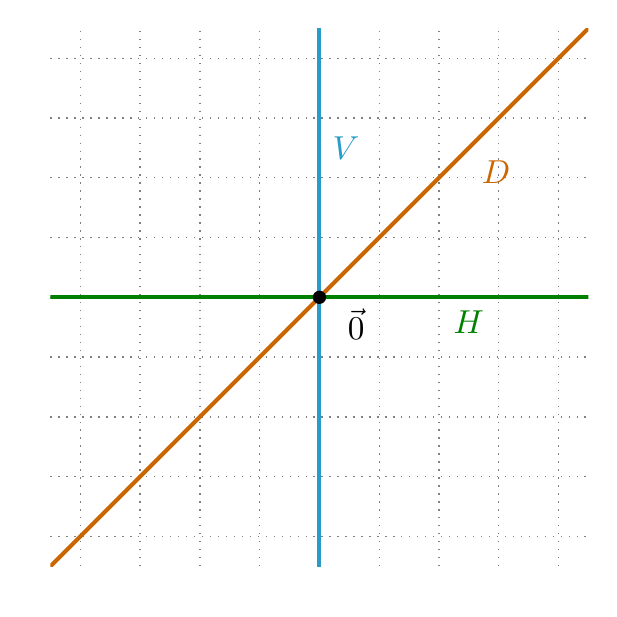
\begin{tikzpicture}[scale=1.2, >=latex]
    \begin{axis}[scale=1,
		    axis equal image,
		    axis line style={draw=none},
		    tick style={draw=none},
		    yticklabels={,,},
		    xticklabels={,,},
		 xmin=-4.5,
		 xmax=4.5,
		 ymin=-4.5,
		 ymax=4.5,
		 major grid style={dotted, gray},
                 xtick={-10,-9,...,10},
                 ytick={-10,-9,...,10},
                 grid=both,
		 anchor=origin]

	    \draw[Green, very thick] (-5,0) -- (5,0) node[near end, below] {$H$};
	    \draw[cyan!80!black, very thick] (0,-5) -- (0,5) node[near end, right] {$V$};
	    \draw[orange!80!black, very thick] (-5,-5) -- (5,5) node[near end, below right] {$D$};

	    \fill[fill=black] (0,0) circle[radius=2pt] node[below right, xshift=5pt] {\color{black}$\vec 0$};
    \end{axis}
\end{tikzpicture}
		\end{solution}
		\item $N=\Set*{\vec x\in\R^2 \given \vec x=t\mat{1\\1}\text{ for all }t\in\R}$.
				\begin{solution}[inline]
			$N=\Set{}$.
		\end{solution}

		\item $V\cup H$.
			\begin{solution}[inline]
			$V\cup H$ looks like a ``$+$'' going through the origin.
		\end{solution}
		\item $V\cap H$.
			\begin{solution}[inline]
				$V\cap H=\Set{\vec 0}$ is just the origin.
		\end{solution}
		\item Does $V\cup H=\R^2$?
			\begin{solution}
				No. $V\cup H$ does not contain $\mat{1\\1}$ while $\R^2$ does contain
				$\mat{1\\1}$.
			\end{solution}
	\end{parts}

\section*{Vector Combinations}
	\vspace{-1em}

	\begin{definition}[Linear Combination]
		A \emph{linear combination} of the vectors $\vec v_1,\vec v_2,\ldots,\vec v_n$ is
		a vector
		\[
			\vec w = \alpha_1\vec v_1+\alpha_2\vec v_2+\cdots+\alpha_n\vec v_n.
		\]
		The scalars $\alpha_1,\alpha_2,\ldots,\alpha_n$ are called the \emph{coefficients} of the linear combination.
	\end{definition}

	\question
	\label{ProbSkewBasis}
	\begin{annotation}
		\begin{goals}
			\Goal{Practice linear combinations.}

			The goal of this problem is to
			\begin{itemize}
				\item Practice using the formal term \emph{linear combination}.
				\item Foreshadow span.
			\end{itemize}
		\end{goals}

		\begin{notes}
			\begin{itemize}
				\item In 2, the question should arise: ``Is $3\vec v_1$
					a linear combination of $\vec v_1$ \emph{and}
					$\vec v_2$?'' Address this.
				\item Refer to the magic carpet ride for 5. You don't
					need to do a full proof.
			\end{itemize}
		\end{notes}
	\end{annotation}
	Let $\vec v_1=\mat{1\\1}$, $\vec v_2=\mat{1\\-1}$, and $\vec w=2\vec v_1+\vec v_2$.
	\begin{parts}
		\item Write $\vec w$ as a column vector. When $\vec w$ is written as a
			linear combination of $\vec v_1$ and $\vec v_2$, what are the
			coefficients of $\vec v_1$ and $\vec v_2$?
			\begin{solution}
				$\vec w=\mat{3\\2}$; the coefficients are $(2,1)$.
			\end{solution}
		\item Is $\mat{3\\3}$ a linear combination of $\vec v_1$ and $\vec v_2$?
			\begin{solution}[inline]
				Yes. $\mat{3\\3}=3\vec v_1+0\vec v_2$.
			\end{solution}

		\item Is $\mat{0\\0}$ a linear combination of $\vec v_1$ and $\vec v_2$?
			\begin{solution}[inline]
				Yes. $\vec 0=0\vec v_1+0\vec v_2$.
			\end{solution}
		\item Is $\mat{4\\0}$ a linear combination of $\vec v_1$ and $\vec v_2$?
			\begin{solution}[inline]
				Yes. $\mat{4\\0}=2\vec v_1+2\vec v_2$.
			\end{solution}
		\item Can you find a vector in $\R^2$ that isn't a linear combination of
		$\vec v_1$ and $\vec v_2$?
			\begin{solution}
				No. $\mat{1\\0}=\tfrac{1}{2}\vec v_1+\tfrac{1}{2}\vec v_2$ and
				$\mat{0\\1}=\tfrac{1}{2}\vec v_1-\tfrac{1}{2}\vec v_2$.
				Therefore
				\[
					\mat{a\\b}
					= a\mat{1\\0}+b\mat{0\\1}
					= a(\tfrac{1}{2}\vec v_1+\tfrac{1}{2}\vec v_2)
						+b(\tfrac{1}{2}\vec v_1-\tfrac{1}{2}\vec v_2)
					=(\tfrac{a+b}{2})\vec v_1+(\tfrac{a-b}{2})\vec v_2.
				\]
				Therefore any vector in $\R^2$ can be written as linear combinations
				of $\vec v_1$ and $\vec v_2$.
			\end{solution}
		\item Can you find a vector in $\R^2$ that isn't a linear combination of
			$\vec v_1$?
			\begin{solution}
				Yes. All linear combinations of $\vec v_1$ have equal $x$ and
				$y$ coordinates, therefore $\vec w=\mat{2\\1}$ is not a linear
				combination of $\vec v_1$.
			\end{solution}
	\end{parts}


	\question
	\begin{annotation}
		\begin{goals}
			\Goal{Practice formal writing.}
		\end{goals}

		\begin{notes}
			\begin{itemize}
				\item Make everyone \emph{write}. They will think
					they can do it, but they will find it hard if
					they try.
			\end{itemize}
		\end{notes}
	\end{annotation}
	Recall the \emph{Magic Carpet Ride} task where the hover board could
	travel in the direction $\vec h=\mat{3\\1}$ and the magic carpet could
	move in the direction $\vec m=\mat{1\\2}$.
	\begin{parts}
		\item Rephrase the sentence \emph{``Gauss can be reached using just the
			magic carpet and the hover board''} using formal mathematical
			language.
			\begin{solution}
				Gauss's location can be written as a linear combination of
				$\vec m$ and $\vec h$.
			\end{solution}
		\item Rephrase the sentence \emph{``There is nowhere Gauss can hide
			where he is inaccessible by magic carpet and hover board''} using
			formal mathematical language.
			\begin{solution}
				Every vector in $\R^2$ can be written as a linear combination
				of $\vec m$ and	$\vec h$.
			\end{solution}
		\item Rephrase the sentence \emph{``$\R^2$ is the set of all linear
			combinations of $\vec h$ and $\vec m$''} using formal mathematical
			language.
			\begin{solution}
				$\R^2=\Set{\vec v\given \vec v=t\vec m+s\vec h\text{ for some }t,s\in \R}$.
			\end{solution}
	\end{parts}

\begin{module}
	\Title{Restricted Linear Combinations, Lines}

	\Heading{Textbook} Section 1.2

	\Heading{Objectives}
	\begin{itemize}
		\item Read and digest a new definition.

		\item Use pictures to explore a new concept.

		\item Convert from an equation-representation of a line to a set-representation.
	\end{itemize}

	\Heading{Motivation} Part of doing math in the world is reading and understanding
	other people's definitions. Most students will not have heard of non-negative
	linear combinations or convex linear combinations. This is a chance for them
	to read and try to understand these formal definitions. They will need to
	draw pictures to get an intuition about what these concepts mean.

	These concepts are useful in their own right, and in particular, convex linear
	combinations can be used to describe line segments. Adding these definitions
	to a student's toolbox serves the goal of \emph{being able to describe
	the world with mathematics}.

	To that end, we start working with lines. Lines are something students have
	used since grade school, but they worked with them in $y=mx+b$ form which
	is only applicable in $\R^{2}$. We want to convert this representation
	into vector form and set-based descriptions which apply to all
	dimensions.

\end{module}

	\displayonlynewpage
	\begin{definition}[Non-negative \& Convex Linear Combinations]
		The linear combination $\vec w=\alpha_1\vec v_1+\alpha_2\vec v_2+\cdots+\alpha_n\vec v_n$ is
		called a \emph{non-negative} linear combination of $\vec v_1,\vec v_2,\ldots,\vec v_n$ if
		$\alpha_1,\alpha_2,\ldots,\alpha_n\geq 0$.

		If $\alpha_1,\alpha_2,\ldots,\alpha_n\geq 0$
		and $\alpha_1+\alpha_2+\cdots+\alpha_n=1$, then $\vec w$ is called a \emph{convex} linear combination
	of  $\vec v_1,\vec v_2,\ldots,\vec v_n$.
	\end{definition}

	\question
	\begin{annotation}
		\begin{goals}
			\Goal{Geometric meaning of \emph{non-negative} and \emph{convex}
			linear
			combinations.}

			The goal of this problem is to
			\begin{itemize}
				\item Read and apply the definition of non-negative and convex
					linear combinations.
				\item Gain geometric intuition for non-negative and convex linear
					combinations.
				\item Learn how to describe line segments using
					convex linear combinations.
			\end{itemize}
		\end{goals}

		\begin{notes}
			\begin{itemize}
				\item This question is about reading and applying;
					emphasize that before they start.
				\item The geometry won't be obvious. Ask them to \emph{draw} specific
					linear combinations (e.g., $(1/2,1/2)$) to get an idea.
				\item They know $\vec a$ and $\vec b$ span all vectors from problem \ref{ProbSkewBasis}.
				\item In part 1, they will forget $\vec a$ and $\vec b$ are linear combinations of themselves.
				\item Part 2 (b) highlights a degeneracy that will come up again when discussing linear independence and dependence. Explain how the 
					picture for non-negative linear combinations
					almost always looks one way, but this case is an exception.
			\end{itemize}
		\end{notes}
	\end{annotation}
	Let
	\[
		\vec a=\mat{1\\1} \qquad \vec b=\mat{-1\\1}\qquad \vec c=\mat{0\\1}\qquad\vec d=\mat{0\\2}\qquad\vec e=\mat{-1\\-1}.
	\]
	\begin{parts}
		\item Out of $\vec a$, $\vec b$, $\vec c$, $\vec d$, and $\vec e$, which
			vectors are
			\begin{enumerate}
				\item linear combinations of $\vec a$ and $\vec b$?
				\begin{solution}[inline]
					All of them, since any vector in $\R^2$ can be written as a linear combination
					of $\vec a$ and $\vec b$.
				\end{solution}

				\item non-negative linear combinations of $\vec a$ and $\vec b$?
				\begin{solution}[inline]
					$\vec a$, $\vec b$, $\vec c$, $\vec d$.
				\end{solution}

				\item convex linear combinations of $\vec a$ and $\vec b$?
				\begin{solution}[inline]
					$\vec a$, $\vec b$, $\vec c$.
				\end{solution}
			\end{enumerate}

		\item If possible, find two vectors $\vec u$ and $\vec v$ so that
			\begin{enumerate}
				\item $\vec a$ and $\vec c$ are non-negative linear combinations
					of $\vec u$ and $\vec v$ but $\vec b$ is not.
				\begin{solution}
					Let $\vec u=\vec a$ and $\vec v=\vec c$.
				\end{solution}

				\item $\vec a$ and $\vec e$ are non-negative linear combinations
					of $\vec u$ and $\vec v$.
				\begin{solution}
					Let $\vec u=\vec a$ and $\vec v=\vec e$.
				\end{solution}

				\item $\vec a$ and $\vec b$ are non-negative linear combinations
					of $\vec u$ and $\vec v$ but $\vec d$ is not.
				\begin{solution}
					Impossible. If $\vec a$ and $\vec b$ are non-negative
					linear combinations of $\vec u$ and $\vec v$, then every non-negative
					linear combination of $\vec a$ and $\vec b$ is also a non-negative
					linear combination of $\vec u$ and $\vec v$. And, we already concluded that
					$\vec d$ is a non-negative linear combination of $\vec a$ and $\vec b$.
				\end{solution}

				\item $\vec a$, $\vec c$, and $\vec d$ are convex linear
					combinations of $\vec u$ and $\vec v$.
				\begin{solution}
					Impossible. Convex linear combinations all lie on the same line segment,
					but $\vec a$, $\vec c$, and $\vec d$ are not collinear.
				\end{solution}
			\end{enumerate}Otherwise, explain why it's not possible.
	\end{parts}

	\displayonlynewpage
\section*{Lines and Planes}

	\question
	\begin{annotation}
		\begin{goals}
			\Goal{Link prior knowledge to new notation/concepts.}

			The goal of this problem is to
			\begin{itemize}
				\item Convert between $y=mx+b$ form of a line and
					the set-builder definition of the same line.
				\item Think about lines in terms of vectors rather
					than equations.
			\end{itemize}
		\end{goals}

		\begin{notes}
			\begin{itemize}
				\item This question is foreshadowing for vector form of a line.
				\item In part 3, some will draw $\vec d$ from the origin and
					some will draw it on the line. Both are fine, but make
					sure they understand that $\vec d\notin L$ by the end of
					part 4.
			\end{itemize}
		\end{notes}
	\end{annotation}
	Let $L$ be the set of points $(x,y)\in\R^2$ such that $y=2x+1$.
	\begin{parts}
		\item Describe $L$ using set-builder notation.
			\begin{solution}
				$\Set*{\vec v\in\R^2 \given \vec v=\matc{t\\2t+1}\text{ for some } t\in\R}$\\
				or
				$\Set*{\mat{x\\y}\in\R^2 \given y=2x+1}$
				or
				$\Set*{\matc{t\\2t+1}\in\R^2 \given t\in\R}$
			\end{solution}
		\item Draw $L$ as a subset of $\R^2$.
		\item Add the vectors $\vec a=\mat{-1\\-1}$, $\vec b=\mat{1\\3}$ and
			$\vec d=\vec b-\vec a$ to your drawing.
			\begin{solution}
				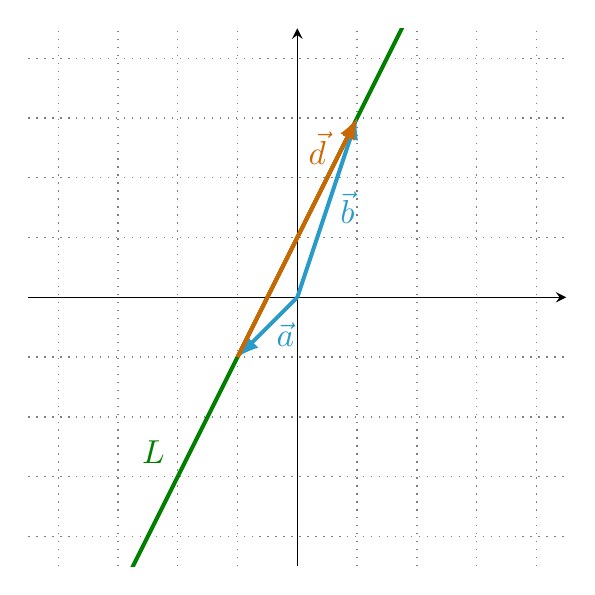
\begin{tikzpicture}[scale=1.2, >=latex]
			    \begin{axis}[scale=1,
					    axis equal image,
					    axis lines=middle,
					    axis line style = {black},
					    tick style={draw=none},
					    yticklabels={,,},
					    xticklabels={,,},
					 xmin=-4.5,
					 xmax=4.5,
					 ymin=-4.5,
					 ymax=4.5,
					 major grid style={dotted, gray},
					 xtick={-10,-9,...,10},
					 ytick={-10,-9,...,10},
					 grid=both,
					 anchor=origin]

				    \draw[Green, very thick] (-5,-9) -- (5,11) node[pos=.3, above left] {$L$};
				    \draw[cyan!80!black, very thick, ->] (0,0) -- (-1,-1) node[pos=.2, below] {$\vec a$};
				    \draw[cyan!80!black, very thick, ->] (0,0) -- (1,3) node[pos=.5, right] {$\vec b$};
				    \draw[orange!80!black, very thick, ->] (-1,-1) -- (1,3) node[near end, above, xshift=-3pt] {$\vec d$};

			    \end{axis}
				\end{tikzpicture}
			\end{solution}
		\item Is $\vec d\in L$? Explain.
			\begin{solution}
				No. $\vec d=\mat{2\\4}$ and so its entries don't satisfy $y=2x+1$.
			\end{solution}
		\item For which $t\in\R$ is it true that $\vec a+t\vec d\in L$? Explain using your picture.
			\begin{solution}
				$\vec a +t\vec d\in L$ for any $t\in \R$. We can see this because if we start at the
				vector $\vec a$ and the displace by $t\vec d$, we will always be on the line $L$.
			\end{solution}
	\end{parts}




%



%%%%%%%%%%%%%%%%%%%%%%%%%%%%%%%%%%%%%%%%%%%%%%%%%%%%%%%%%%%%%%%%%%%%%%%%
%
%		Appendices
%
%%%%%%%%%%%%%%%%%%%%%%%%%%%%%%%%%%%%%%%%%%%%%%%%%%%%%%%%%%%%%%%%%%%%%%%%




%\appendix


\begin{topic}[Appendix]

\end{topic}


\subsection{2019 $M_3C$ competition report from the winning team}
\label{2019M3C}

%\hspace{-0.5cm}\includegraphics*[page=1,scale=0.9]{example/Vaping-abridged.pdf}
%
%\newpage

In the folowing pages you can find an abridged version of the full report. The full report can be found at \href{http://uoft.me/modelling-app-report}{http://uoft.me/modelling-app-report}.

	\vfil

	\hfil \framebox{\includegraphics*[scale=0.67]{example/Vaping-cover.pdf}}

\newpage

\forLoop[1]{1}{12} % variable is \i
{
	\hfil\\
	\vfil
	\hfil \framebox{\includegraphics*[page=\i,scale=0.85]{example/Vaping-abridged.pdf}}
	\newpage
}






\end{document}
